%%%%%%%%%%%%%%%%%%%%%%%%%%%%%%%%%%%%%%%%
% Masters/Doctoral Thesis 
% LaTeX Template
% Version 2.5 (27/8/17)
%
% This template was downloaded from:
% http://www.LaTeXTemplates.com
%
% Version 2.x major modifications by:
% Vel (vel@latextemplates.com)
%
% This template is based on a template by:
% Steve Gunn (http://users.ecs.soton.ac.uk/srg/softwaretools/document/templates/)
% Sunil Patel (http://www.sunilpatel.co.uk/thesis-template/)
%
% Template license:
% CC BY-NC-SA 3.0 (http://creativecommons.org/licenses/by-nc-sa/3.0/)
%
%%%%%%%%%%%%%%%%%%%%%%%%%%%%%%%%%%%%%%%%%

%----------------------------------------------------------------------------------------
%	PACKAGES AND OTHER DOCUMENT CONFIGURATIONS
%----------------------------------------------------------------------------------------

\documentclass[
11pt, % The default document font size, options: 10pt, 11pt, 12pt
oneside, % Two side (alternating margins) for binding by default, uncomment to switch to one side
spanish, % ngerman for German
singlespacing, % Single line spacing, alternatives: onehalfspacing or doublespacing
%draft, % Uncomment to enable draft mode (no pictures, no links, overfull hboxes indicated)
%nolistspacing, % If the document is onehalfspacing or doublespacing, uncomment this to set spacing in lists to single
%liststotoc, % Uncomment to add the list of figures/tables/eta, haberc to the table of contents
%toctotoc, % Uncomment to add the main table of contents to the table of contents
parskip, % Uncomment to add space between paragraphs
%nohyperref, % Uncomment to not load the hyperref package
headsepline, % Uncomment to get a line under the header
%chapterinoneline, % Uncomment to place the chapter title next to the number on one line
%consistentlayout, % Uncomment to change the layout of the declaration, abstract and acknowledgements pages to match the default layout
table
]{MastersDoctoralThesis} % The class file specifying the document structure


\usepackage{xcolor}

\usepackage{soul}
\usepackage{graphicx}
%\usepackage{subfig}

\usepackage[bottom]{footmisc}

\usepackage[utf8]{inputenc} % Required for inputting international characters
%\usepackage[T1]{fontenc} % Output font encoding for international characters

\usepackage{mathpazo} % Use the Palatino font by default

\usepackage{amssymb} % For \checkmark in tables
\usepackage{multirow} % For multi-row cells in tables
\usepackage{booktabs} % For professional tables

\usepackage{caption}

\usepackage{float}

\usepackage{hyperref}
\usepackage{apacite} %EN CASO DE NO USAR APA STYLE COMENTAR ESTA LINEA Y CAMBIAR EL ESTILO DE ABAJO

%\usepackage{subcaption}

%\usepackage[backend=bibtex, natbib=true]{biblatex} % Use the bibtex backend with the authoryear citation style (which resembles APA)
% SI AGREGO STYLE=AUTHORYEAR PARA QUE SEA ESTILO APA, SE ME DESORDENA EL FORMATO DE LOS AUTORES EN LA BIBLIOGRAFIA... MUY RARO, NO ENCUENTRO SOLUCION EN GOOGLE HASTA EL MOMENTO
%\usepackage[
%backend=biber,
%style=alphabetic,
%citestyle=authoryear
%]{biblatex}

% Use the bibtex backend with the authoryear citation style (which resembles APA)
%,style=authoryear,natbib=true

%\addbibresource{citas.bib} % The filename of the bibliography
%\usepackage[autostyle=true]{csquotes} % Required to generate language-dependent quotes in the bibliography
%\usepackage{color}
%----------------------------------------------------------------------------------------
%	MARGIN SETTINGS
%----------------------------------------------------------------------------------------

\geometry{
	paper=a4paper, % Change to letterpaper for US letter
	inner=2.5cm, % Inner margin
	outer=3.8cm, % Outer margin
	bindingoffset=.5cm, % Binding offset
	top=1.5cm, % Top margin
	bottom=1.5cm, % Bottom margin
	%showframe, % Uncomment to show how the type block is set on the page
}

%----------------------------------------------------------------------------------------
%	THESIS INFORMATION
%----------------------------------------------------------------------------------------

\thesistitle{Aumentación de Datos con LLMs: Filtrado Geométrico para Clasificación de Texto} % Your thesis title, this is used in the title and abstract, print it elsewhere with \ttitle
\thesistitleEnglish{Data Augmentation with LLMs: Geometric Filtering for Text Classification} % Your thesis title, this is used in the title and abstract, print it elsewhere with \ttitleEnglish
\supervisor{Gonzalo Ruz} % Your supervisor's name, this is used in the title page, print it elsewhere with \supname
\examiner{NOMBRE COMISON\\2DO NOMBRE COMISION} % Your examiner's name, this is not currently used anywhere in the template, print it elsewhere with \examname
\degree{Master of Science in Data Science} % Your degree name, this is used in the title page and abstract, print it elsewhere with \degreename
\degreeEnglish{Master of Science in Data Science}
\author{Benjamín Schindler} % Your name, this is used in the title page and abstract, print it elsewhere with \authorname
\addresses{} % Your address, this is not currently used anywhere in the template, print it elsewhere with \addressname
\subject{Machine Learning} % Your subject area, this is not currently used anywhere in the template, print it elsewhere with \subjectname
\keywords{clasificación de texto, aumentación de datos, modelos de lenguaje, filtrado geométrico, embeddings, SMOTE, pocos ejemplos} % Keywords for your thesis, this is not currently used anywhere in the template, print it elsewhere with \keywordnames
\university{\href{https://www.uai.cl/}{Universidad Adolfo Ibañez}} % Your university's name and URL, this is used in the title page and abstract, print it elsewhere with \univname
\department{\href{https://ingenieria.uai.cl/}{Facultad de Ingeniería y Ciencias}} % Your department's name and URL, this is used in the title page and abstract, print it elsewhere with \deptname
\faculty{\href{https://ingenieria.uai.cl/}{Facultad de Ingeniería y Ciencias}} % Your faculty's name and URL, this is used in the title page and abstract, print it elsewhere with \facname
\facultyEnglish{\href{https://ingenieria.uai.cl/}{Faculty of Engineering and Science}} % Your faculty's name and URL, this is used in the title page and abstract, print it elsewhere with \facname

\AtBeginDocument{
\hypersetup{pdftitle=\ttitle} % Set the PDF's title to your title
\hypersetup{pdfauthor=\authorname} % Set the PDF's author to your name
\hypersetup{pdfkeywords=\keywordnames} % Set the PDF's keywords to your keywords
}

\begin{document}

\frontmatter % Use roman page numbering style (i, ii, iii, iv...) for the pre-content pages

\pagestyle{plain} % Default to the plain heading style until the thesis style is called for the body content

%----------------------------------------------------------------------------------------
%	TITLE PAGE
%----------------------------------------------------------------------------------------

\begin{titlepage}
\begin{center}

\vspace*{.04\textheight}
{\scshape\LARGE \univname\par}\vspace{1cm} % University name
\textsc{\Large Tesis de Magíster}\\[0.4cm] % Thesis type

\HRule \\[0.3cm] % Horizontal line
{\LARGE \bfseries \ttitle\par}\vspace{0.3cm} % Thesis title
\HRule \\[1cm] % Horizontal line
 
\begin{minipage}[t]{0.4\textwidth}
\begin{flushleft} \large
\emph{Autor:}\\
{\authorname} % Author name - remove the \href bracket to remove the link
\end{flushleft}
\end{minipage}
\begin{minipage}[t]{0.4\textwidth}
\begin{flushright} \large
\emph{Profesor guía:} \\
\supname\\
\vspace{5mm}
\emph{Comité de defensa:} \\
\examname\\
%\href{https://ingenieria.uai.cl/profesor/paginaWeb1/}{\supname} \\% Supervisor name - remove the \href bracket to remove the link  
%\href{https://ingenieria.uai.cl/profesor/paginaWeb2/}{\examname} % Supervisor name - remove the \href bracket to remove the link  
\end{flushright}
\end{minipage}\\[1.5cm]
 
\vfill

\large \textit{Tesis realizada acorde a los requerimientos para el grado de\\  \degreename}\\[0.3cm] % University requirement text
\textit{de la}\\[0.4cm]
\facname\\[0.8cm] % Research group name and department name
 
\vfill

{\large \today}\\[0.8cm] % Date

\includegraphics[width=4cm]{fic.png} % University/department logo

\end{center}
\end{titlepage}

%----------------------------------------------------------------------------------------
%	ABSTRACT PAGE
%----------------------------------------------------------------------------------------

\begin{resumen}
\addchaptertocentry{\abstractname} % Add the abstract to the table of contents

La clasificación de texto en escenarios de recursos limitados enfrenta un desafío fundamental: la escasez de datos etiquetados impide que los clasificadores aprendan fronteras de decisión robustas, especialmente en problemas multiclase. Los modelos de lenguaje de gran escala (LLMs) pueden generar texto sintético para aumentar los datos de entrenamiento, pero no todas las muestras generadas son igualmente útiles. Algunas se ubican en regiones del espacio de embeddings que no corresponden a la clase objetivo, mientras que otras carecen de diversidad suficiente.

Esta tesis propone un sistema de filtrado geométrico que evalúa las muestras sintéticas generadas por LLMs según su posición en el espacio de embeddings. El sistema implementa múltiples filtros basados en distancia euclidiana, densidad local y coherencia con la distribución de datos reales. Adicionalmente, se introduce un mecanismo de ponderación suave que utiliza las puntuaciones del filtro como pesos de muestra en el clasificador, asignando mayor importancia a las muestras de mayor calidad geométrica.

La evaluación experimental abarca 3,675 configuraciones sobre 7 conjuntos de datos de clasificación, 5 clasificadores, 7 métodos de aumentación y 5 semillas. El método propuesto obtiene +2.25 puntos porcentuales sobre SMOTE ($p<0.0001$, $d$ de Cohen = 0.74, tasa de victoria 83.8\%), superando también a 9 líneas base incluyendo técnicas modernas como paráfrasis con T5 y aumentación contextual con BERT. La extensión a reconocimiento de entidades nombradas confirma la generalización del enfoque, con +9.61 puntos porcentuales sobre la línea base.

Un hallazgo central es que los filtros simples basados únicamente en distancia superan a los filtros complejos multi-criterio, y que las ganancias son mayores en escenarios de máxima escasez (10 ejemplos por clase: +4.52pp).

\textbf{Palabras clave:} clasificación de texto, aumentación de datos, modelos de lenguaje, filtrado geométrico, embeddings, SMOTE, pocos ejemplos.
\end{resumen}

\begin{abstract}
\addchaptertocentry{Abstract} % Add the abstract to the table of contents

Text classification in low-resource scenarios faces a fundamental challenge: the scarcity of labeled data prevents classifiers from learning robust decision boundaries, especially in multi-class problems. Large language models (LLMs) can generate synthetic text to augment training data, but not all generated samples are equally useful. Some fall in embedding space regions that do not correspond to the target class, while others lack sufficient diversity.

This thesis proposes a geometric filtering system that evaluates LLM-generated synthetic samples based on their position in the embedding space. The system implements multiple filters based on Euclidean distance, local density, and coherence with the real data distribution. Additionally, a soft weighting mechanism is introduced that uses filter scores as sample weights in the classifier, assigning greater importance to samples of higher geometric quality.

The experimental evaluation spans 3,675 configurations across 7 classification datasets, 5 classifiers, 7 augmentation methods, and 5 seeds. The proposed method achieves +2.25 percentage points over SMOTE ($p<0.0001$, Cohen's $d$ = 0.74, win rate 83.8\%), also outperforming 9 baselines including modern techniques such as T5 paraphrasing and contextual BERT augmentation. The extension to named entity recognition confirms the generalization of the approach, with +9.61 percentage points over baseline.

A central finding is that simple distance-based filters outperform complex multi-criteria filters, and that gains are largest in maximum scarcity scenarios (10 examples per class: +4.52pp).

\textbf{Keywords:} text classification, data augmentation, language models, geometric filtering, embeddings, SMOTE, few-shot.

\end{abstract}

%----------------------------------------------------------------------------------------
%	ACKNOWLEDGEMENTS
%----------------------------------------------------------------------------------------

\begin{acknowledgements}
\addchaptertocentry{\acknowledgementname}

Agradezco profundamente a mi familia, a mi pareja y a mis amigos por su apoyo incondicional durante este proceso. Su paciencia, motivación y compañía fueron fundamentales para llevar a cabo esta investigación.

También agradezco el financiamiento de: ANID FONDECYT 1230315, ANID-MILENIO-NCN2024\_103; y CMM FB210005, correspondientes a fondos BASAL para centros de excelencia de ANID-Chile.

\end{acknowledgements}

%----------------------------------------------------------------------------------------
%	LIST OF CONTENTS/FIGURES/TABLES PAGES
%----------------------------------------------------------------------------------------

\tableofcontents % Prints the main table of contents

%\listoffigures % Prints the list of figures

%\listoftables % Prints the list of tables

%----------------------------------------------------------------------------------------
%	ABBREVIATIONS
%----------------------------------------------------------------------------------------

%\begin{abbreviations}{ll} % Include a list of abbreviations (a table of two columns)

%\textbf{ACHS} & \textbf{A}sicación \textbf{C}hilena \textbf{D}e \textbf{S}eguridad\\
%\textbf{SUSESO} & \textbf{S}uperintendencia \textbf{D}e \textbf{S}eguridad \textbf{S}ocial\\
%\textbf{MUSEG} & \textbf{M}utual \textbf{D}e \textbf{S}eguridad \textbf{D}e \textbf{L}a \textbf{C}ámara \textbf{C}hilena \textbf{D}e \textbf{L}a  \textbf{C}onstrucción \\

%\end{abbreviations}

%----------------------------------------------------------------------------------------
%	THESIS CONTENT - CHAPTERS
%----------------------------------------------------------------------------------------

\mainmatter % Begin numeric (1,2,3...) page numbering

\pagestyle{thesis} % Return the page headers back to the "thesis" style

% Include the chapters of the thesis as separate files from the Chapters folder
% Uncomment the lines as you write the chapters

% Chapter 1
\chapter{Introducción} % Main chapter title
\label{sec:Introduccion} % For referencing the chapter elsewhere, use

La era digital ha transformado radicalmente la forma en que las personas expresan y comparten sus opiniones. Cada día, millones de usuarios publican reseñas de productos, comentarios en redes sociales y opiniones sobre servicios en plataformas digitales. Este fenómeno ha generado un volumen sin precedentes de texto no estructurado que contiene información valiosa sobre la percepción pública. Las organizaciones modernas dependen cada vez más de esta información para tomar decisiones estratégicas: desde ajustar características de productos hasta gestionar crisis de reputación en tiempo real \cite{liu2015sentiment}.

El análisis de sentimientos se ha consolidado como la técnica fundamental para interpretar esta avalancha de opiniones. Su capacidad para clasificar automáticamente texto según polaridad emocional (positiva, negativa, neutra) permite a empresas y gobiernos monitorear la satisfacción del cliente, detectar tendencias emergentes y responder proactivamente a problemas antes de que escalen. Sin embargo, la efectividad de estos sistemas enfrenta un obstáculo metodológico persistente: el desbalance de clases.

En la mayoría de datasets de sentimientos ampliamente utilizados, la distribución de opiniones dista de ser uniforme. Conjuntos de referencia como Stanford Sentiment Treebank 2, TASS-SEPLN y Coursera Reviews exhiben consistentemente una clase mayoritaria que representa más del 60\% de las muestras \cite{gopali2024applicability}. Este desequilibrio no es meramente un inconveniente técnico. Provoca que los modelos converjan hacia estrategias que favorecen sistemáticamente la clase dominante, sacrificando su capacidad para identificar opiniones minoritarias. El resultado es una degradación pronunciada en métricas como el macro F1-score, comprometiendo la utilidad práctica de estos sistemas en escenarios donde detectar cada tipo de sentimiento es igualmente crítico \cite{gopali2024applicability,whitehouse2023llm}.

\subsection{Enfoques Existentes para el Desbalance de Clases}

La comunidad científica ha desarrollado dos paradigmas principales para abordar este desafío. Las técnicas clásicas de oversampling, ejemplificadas por SMOTE (Synthetic Minority Oversampling Technique) y ADASYN (Adaptive Synthetic Sampling), operan mediante interpolación lineal en espacios vectoriales de embeddings \cite{chawla2002smote,he2008adasyn}. Estos métodos identifican ejemplos de la clase minoritaria y generan muestras sintéticas interpolando entre vecinos cercanos en el espacio de representación. Cuando se combinan con clasificadores basados en modelos transformers como BERT, estas técnicas logran mejoras significativas en F1-score \cite{cloutier2023fine,devlin2018bert}.

Por otro lado, los avances recientes en Large Language Models (LLMs) han abierto una vía alternativa. Modelos como GPT-3 y GPT-4 poseen capacidades generativas que permiten crear texto nuevo directamente a partir de descripciones o ejemplos de la clase minoritaria. La investigación de Suhaeni y Yong demostró que agregar reseñas sintéticas generadas por GPT-3 al corpus Coursera Reviews produjo incrementos de 12.7\% en exactitud media y hasta 13 puntos porcentuales en macro F1-score \cite{suhaeni2023mitigating}. Estos modelos generan texto gramaticalmente correcto que preserva naturalidad lingüística, superando la limitación fundamental de los métodos de interpolación: la falta de correspondencia entre vectores interpolados y texto lingüísticamente válido \cite{whitehouse2023llm}.

Cada paradigma presenta fortalezas complementarias. SMOTE y ADASYN proporcionan guía geométrica explícita sobre dónde posicionar muestras sintéticas en el espacio de embeddings, identificando estratégicamente regiones subrepresentadas. Los LLMs, en contraste, generan texto coherente y diverso, pero operan sin información sobre la estructura geométrica del espacio de representación. Esta complementariedad ha motivado el surgimiento de metodologías híbridas emergentes.

\subsection{El Paradigma Híbrido Emergente}

Arquitecturas recientes han comenzado a integrar técnicas clásicas con capacidades generativas de LLMs. SMOTExT propone utilizar SMOTE para identificar puntos de interpolación en el espacio de embeddings, luego emplear un LLM para generar texto correspondiente a esas ubicaciones geométricas \cite{smotext2025arxiv}. De manera similar, ImbLLM explora la capacidad de LLMs para generar muestras sintéticas guiadas por información estructural del dataset \cite{imbllm2024arxiv}. Estos trabajos han establecido las bases conceptuales del paradigma híbrido, demostrando que entrenar exclusivamente con datos sintéticos puede lograr rendimientos cercanos a baselines con datos reales, con degradaciones de aproximadamente 3.2\% en algunos casos.

A pesar de estos avances prometedores, el análisis de la literatura revela que los enfoques híbridos actuales aún presentan limitaciones metodológicas que restringen su efectividad. Estas limitaciones se detallan en la sección de Definición del Problema y constituyen la motivación principal de esta investigación.

\subsection{Contribución de Esta Investigación}

Esta tesis propone una arquitectura híbrida avanzada que integra cuatro innovaciones metodológicas diseñadas para superar las limitaciones identificadas en enfoques previos. Primero, implementa una selección de soporte ponderada que utiliza un número mayor de vecinos contextualmente relevantes para proporcionar información más rica al LLM durante la generación. Segundo, incorpora un sistema de filtrado multi-nivel adaptativo que valida la calidad de las muestras sintéticas mediante criterios complementarios aplicados en cascada. Tercero, aplica ponderación basada en confianza geométrica, donde cada muestra sintética recibe peso proporcional a indicadores de su contexto local en el espacio de embeddings. Finalmente, el diseño enfatiza la eficiencia computacional mediante generación directa con LLMs pre-entrenados sin requerir fine-tuning.

El objetivo principal es evaluar sistemáticamente, mediante estudios de ablación rigurosos en múltiples datasets con diversos grados de desbalance, las contribuciones individuales de cada componente y la efectividad del sistema integrado en tareas de clasificación de sentimientos. Esta investigación busca proporcionar un protocolo reproducible que guíe la selección de técnicas según características del dataset y restricciones operacionales, contribuyendo tanto al avance científico en el equilibrio de clases como a la aplicabilidad práctica en sistemas de producción que requieren predicciones confiables en todas las categorías de sentimiento.
% Chapter 2 - Definición del Problema

\chapter{Definición del Problema}
\label{ch:problema}

\section{El Problema de la Escasez de Datos Etiquetados}

La clasificación supervisada de texto requiere ejemplos etiquetados en cantidad suficiente para que el modelo aprenda los patrones distintivos de cada clase. En la práctica, muchas tareas disponen de conjuntos de entrenamiento extremadamente reducidos. Un investigador que desea construir un detector de discurso de odio para una plataforma nueva, o un clasificador de intenciones para un dominio especializado, puede contar con apenas 10 a 50 ejemplos etiquetados por categoría. Esta situación, denominada escenario de pocos ejemplos, impide que los algoritmos de aprendizaje estadístico estimen con precisión las fronteras de decisión entre clases.

La degradación del rendimiento es especialmente severa en problemas multiclase. Cuando el espacio de categorías se amplía, cada clase necesita masa crítica independiente para que el modelo capture sus características. Con 10 ejemplos por clase y 6 categorías, el conjunto de entrenamiento completo contiene apenas 60 muestras, una cifra que resulta insuficiente para la mayoría de los algoritmos. Los clasificadores entrenados bajo estas condiciones convergen hacia estrategias que favorecen las clases mejor representadas, produciendo una caída pronunciada en la métrica macro F1 \cite{gopali2024applicability}. Esta métrica, al ponderar equitativamente el rendimiento de cada clase, refleja con fidelidad la incapacidad del modelo para tratar adecuadamente las categorías con menos ejemplos.

El problema no se limita a un dominio particular. Conjuntos de datos ampliamente utilizados en la comunidad, como Stanford Sentiment Treebank 2, AG News, 20 Newsgroups y datasets de detección de spam, presentan distribuciones desiguales entre sus clases \cite{whitehouse2023llm}. La escasez de datos etiquetados y el desbalance entre categorías constituyen así un obstáculo transversal que afecta a múltiples áreas del procesamiento de lenguaje natural.

\section{Limitaciones de las Soluciones Existentes}

La comunidad ha propuesto diversas estrategias de aumentación de datos para mitigar la escasez, pero cada una presenta limitaciones que restringen su efectividad. A continuación se identifican tres deficiencias críticas en los enfoques actuales que motivan esta investigación.

\subsection{Deficiencia 1: Ausencia de Validación Post-Generación}

Los métodos actuales que utilizan LLMs para aumentación de datos aceptan todas las muestras generadas sin evaluar su calidad en el espacio de representación. Un LLM puede producir una oración gramaticalmente correcta que, al ser proyectada al espacio de embeddings, se ubique en una región que corresponde a una clase diferente de la solicitada. De manera análoga, el modelo puede generar texto que cae en zonas periféricas del espacio, alejadas de la distribución real de la clase objetivo.

Esta ausencia de control de calidad geométrico permite que muestras defectuosas contaminen el conjunto de entrenamiento. SMOTExT, por ejemplo, genera texto correspondiente a puntos interpolados en el espacio de embeddings, pero no verifica si el texto producido mantiene coherencia semántica con su ubicación geométrica pretendida \cite{smotext2025arxiv}. La literatura carece de protocolos estandarizados para cuantificar y filtrar estas inconsistencias antes de incorporar las muestras al entrenamiento.

\subsection{Deficiencia 2: Ponderación Uniforme de Muestras Sintéticas}

Los métodos existentes asignan peso idéntico a todas las muestras sintéticas durante el entrenamiento del clasificador. Esta práctica ignora información geométrica disponible que podría mejorar la calidad del aprendizaje. Una muestra sintética ubicada en una región densa del espacio de embeddings, rodeada de múltiples ejemplos reales de su clase, posee mayor probabilidad de ser representativa y confiable. En contraste, una muestra ubicada en una zona dispersa, con pocos vecinos de la misma clase, podría corresponder a un caso atípico o a un error de generación.

Asignar peso uniforme a ambas muestras desaprovecha la señal que proporciona el contexto geométrico local. La información sobre la densidad del vecindario, la distancia a los ejemplos reales más cercanos y la proporción de vecinos de la misma clase constituyen indicadores de calidad que los métodos actuales no explotan. ImbLLM reconoce implícitamente este problema al enfatizar la diversidad durante la generación \cite{imbllm2024arxiv}, pero no implementa esquemas de ponderación adaptativa basados en métricas geométricas locales.

\subsection{Deficiencia 3: Falta de Validación Multi-Tarea y Multi-Dominio}

La mayoría de los estudios que evalúan la aumentación con LLMs se limitan a un solo conjunto de datos o a un único tipo de tarea. Los resultados obtenidos en un corpus particular no garantizan que el método funcione en otros dominios textuales con características diferentes. Esta falta de validación cruzada impide determinar si las ganancias observadas son genuinamente atribuibles al método propuesto o si dependen de particularidades del conjunto de datos empleado.

La carencia es aún más pronunciada cuando se considera la generalización entre tareas. Un mecanismo de control de calidad diseñado para clasificación de texto podría no funcionar para reconocimiento de entidades nombradas, generación de preguntas u otras tareas de procesamiento de lenguaje natural. Hasta la fecha, no se ha demostrado que los filtros de calidad basados en propiedades geométricas del espacio de embeddings mantengan su efectividad a través de tareas y dominios distintos.

\section{Oportunidad de Investigación}

Las deficiencias identificadas revelan una oportunidad en la intersección de tres dimensiones metodológicas. La primera dimensión consiste en integrar mecanismos de validación post-generación que evalúen cada muestra sintética según su posición en el espacio de embeddings, filtrando aquellas que no satisfacen criterios geométricos de calidad. La segunda dimensión propone desarrollar esquemas de ponderación adaptativa que asignen a cada muestra un peso proporcional a su calidad geométrica, en lugar de la decisión binaria de aceptar o rechazar. La tercera dimensión busca demostrar que estos mecanismos de control de calidad generalizan a través de múltiples conjuntos de datos y tareas del procesamiento de lenguaje natural.

Esta tesis aborda sistemáticamente estas tres dimensiones. El sistema propuesto implementa filtros geométricos que operan sobre el espacio de embeddings, un mecanismo de ponderación suave basado en las puntuaciones de dichos filtros, y una validación experimental que abarca 7 dominios textuales y 2 tareas distintas (clasificación y reconocimiento de entidades nombradas). El diseño enfatiza la eficiencia operacional, utilizando LLMs pre-entrenados sin requerir fine-tuning, lo que facilita su aplicación en entornos con recursos computacionales limitados.

% Chapter 1

\chapter{Estado del arte} % Main chapter title
\label{sec:Estado Arte} % For referencing the chapter elsewhere, use

\subsection{El Desbalance de Clases como Barrera Metodológica Persistente}

El desequilibrio de clases representa un desafío fundamental para la validez de los modelos de análisis de sentimientos. Este problema se manifiesta de manera consistente en corpora ampliamente utilizados donde la clase mayoritaria habitualmente excede el 70\% de las muestras. En conjuntos de referencia como Stanford Sentiment Treebank 2, TASS-SEPLN y Coursera Reviews, la ausencia de mecanismos correctivos provoca caídas pronunciadas en el macro F1-score y degradación generalizada del rendimiento \cite{gopali2024applicability}.

Este fenómeno trasciende barreras lingüísticas y dominios específicos. La subrepresentación de clases minoritarias conduce sistemáticamente a predicciones inexactas y bajo rendimiento del modelo para opiniones poco frecuentes \cite{gopali2024applicability,whitehouse2023llm}. La problemática no se limita meramente a métricas de exactitud global. Por el contrario, compromete la utilidad práctica de los sistemas al enmascarar su incapacidad fundamental para identificar patrones en categorías minoritarias, afectando tanto la precisión como la aplicabilidad en escenarios de producción.

Durante más de una década, este desequilibrio ha constituido una barrera metodológica reconocida por la comunidad científica \cite{gopali2024applicability}. La optimización ingenua de la exactitud global induce a los modelos a converger hacia estrategias que favorecen la predicción de la clase dominante, relegando sistemáticamente las opiniones minoritarias. La literatura reciente ha cristalizado las soluciones propuestas en cuatro corrientes metodológicas principales, cada una con fortalezas y limitaciones específicas que fundamentan la necesidad de enfoques híbridos más sofisticados.

\subsection{Taxonomía de Enfoques para Desbalance de Clases en Análisis de Sentimientos}

La investigación contemporánea ha desarrollado cuatro paradigmas fundamentales para abordar el desbalance de clases. Cada paradigma opera en diferentes niveles de abstracción y presenta compensaciones (trade-offs) distintas entre costo computacional, naturalidad lingüística y efectividad empírica.

\subsection{Remuestreo Geométrico Clásico en Espacios de Características}

El remuestreo geométrico constituye el enfoque más establecido. Algoritmos como SMOTE (Synthetic Minority Over-sampling Technique) \cite{chawla2002smote} y ADASYN (Adaptive Synthetic Sampling) \cite{he2008adasyn} generan muestras sintéticas mediante interpolación lineal en espacios vectoriales. Estudios recientes han documentado mejoras significativas en F1-score cuando SMOTE se aplica en conjunto con clasificadores basados en BERT para tareas de clasificación multiclase desbalanceadas \cite{cloutier2023fine}. La aplicación de estas técnicas busca mejorar la exhaustividad (recall) de clases minoritarias sin comprometer excesivamente la precisión global \cite{chawla2002smote,he2008adasyn}.

Sin embargo, investigaciones específicas en clasificación de texto han revelado limitaciones fundamentales de este paradigma. Cuando SMOTE opera exclusivamente en espacios de embeddings textuales, los vectores interpolados resultantes pueden carecer de correspondencia directa con texto lingüísticamente coherente. Esta restricción limita su utilidad en aplicaciones que requieren inspección humana o retokenización para propósitos secundarios. Un estudio comparativo exhaustivo utilizando datos de hoteles demostró que, aunque SMOTE integrado con métodos de ensemble alcanzó 88\% de precisión \cite{putra2025optimizing}, la naturalidad lingüística de los ejemplos sintéticos permanece como preocupación no resuelta.

Análisis adicionales en clasificación textual revelaron que SMOTE aplicado sobre vectores MiniLM produjo mejoras del 17\% al 20\% en recall, particularmente beneficiosas para clases minoritarias \cite{taskiran2025comprehensive}. No obstante, estos resultados vienen acompañados de una salvedad crítica: los puntos interpolados en espacios de alta dimensionalidad no garantizan validez semántica. Las estrategias complementarias de submuestreo (undersampling), como el submuestreo aleatorio (RUS), aunque reducen el sesgo hacia la clase mayoritaria, lo hacen a expensas de descartar información potencialmente valiosa. Este compromiso ha motivado la exploración de enfoques de selección más estratégicos y técnicas de ensamble que intentan preservar información mientras mitigan el desbalance.

\subsection{Sobremuestreo en Espacios de Características Profundas}

El segundo paradigma opera directamente sobre representaciones contextualizadas generadas por modelos transformer. Este enfoque interpola vectores producidos por arquitecturas como BERT \cite{devlin2018bert} con el objetivo explícito de preservar información semántica durante el proceso de síntesis. El método reconoce que los embeddings contextualizados capturan relaciones semánticas más ricas que representaciones basadas en frecuencia de palabras o embeddings estáticos.

Investigaciones recientes han validado este principio mediante implementación de Synthetic Feature Augmentation, que aplica variantes de SMOTE (incluyendo Borderline-SMOTE y ADASYN) directamente en espacios de embeddings BERT sin decodificación a texto \cite{synthetic2025feature}. Los resultados en clasificación binaria (IMDB, SST-2) y multiclase (AG News con cuatro categorías) demostraron que modelos aumentados con SMOTE superaron consistentemente baselines desbalanceados. Las mejoras fueron particularmente pronunciadas cuando el tamaño de la clase minoritaria es extremadamente reducido.

Visualizaciones mediante UMAP y t-SNE confirmaron que muestras sintéticas efectivamente llenan regiones de clase minoritaria manteniendo estructura de cluster y coherencia semántica. La contribución conceptual clave de este enfoque radica en demostrar que técnicas tradicionales de SMOTE, cuando se aplican a embeddings semánticos aprendidos en lugar de características crudas, permanecen altamente efectivas para tareas de procesamiento de lenguaje natural. A diferencia de metodologías que decodifican vectores interpolados a texto, este paradigma opera exclusivamente en espacio de embeddings, ofreciendo eficiencia computacional superior pero sacrificando interpretabilidad directa de las muestras sintéticas generadas.

\subsection{Generación de Texto Completo con Modelos de Lenguaje de Gran Escala}

El tercer paradigma aprovecha la capacidad de los Large Language Models para generar directamente texto completo, gramaticalmente correcto y contextualmente coherente que enriquece las clases minoritarias. Este enfoque ha demostrado ventajas sustanciales sobre métodos geométricos tradicionales en múltiples dimensiones.

La investigación seminal de Suhaeni y Yong documentó que la adición de reseñas sintéticas generadas por GPT-3 al corpus Coursera Reviews produjo incrementos del 12.7\% en exactitud media y hasta 13\% en macro F1-score \cite{suhaeni2023mitigating}. Este resultado estableció un benchmark crítico que motivó investigación subsecuente en múltiples contextos lingüísticos. En el dominio árabe, investigadores utilizaron AraGPT-2 para mejorar la detección de opiniones negativas en contenido de redes sociales \cite{habbat2023using}. Paralelamente, estudios multilingües demostraron mejoras de hasta 13.4\% en exactitud para tareas con datos de entrenamiento limitados, entrenando modelos más pequeños sobre datos sintetizados por GPT-4 \cite{whitehouse2023llm}.

Las comparaciones directas entre LLMs y remuestreo geométrico han revelado ventajas sistemáticas del primer enfoque. Gopali et al. alcanzaron F1-score de 0.76 utilizando GPT-3.5-Turbo, contrastando favorablemente con valores de 0.60 o inferiores obtenidos mediante combinaciones de SMOTE y Edited Nearest Neighbors en el corpus MBTI \cite{gopali2024applicability}. Investigación adicional de Cloutier y Japkowicz demostró que el sobremuestreo mediante LLMs generativos con fine-tuning (específicamente GPT-2) generalmente supera métodos de remuestreo tradicionales en clasificación multiclase desbalanceada \cite{cloutier2023fine}. Sin embargo, esta ventaja resulta menos pronunciada en clasificación binaria, y el fine-tuning del LLM emerge como paso crucial para la efectividad.

La calidad de datos generados constituye factor determinante del rendimiento. Evaluaciones humanas han destacado la capacidad de modelos como ChatGPT y GPT-4 para generar texto natural en múltiples lenguas, ocasionalmente superando la naturalidad de datos originales \cite{whitehouse2023llm}. No obstante, estas evaluaciones también señalan desafíos persistentes en consistencia lógica para ciertos idiomas de bajos recursos y mantenimiento de coherencia comparada con ejemplos producidos por humanos. Los LLMs de última generación capturan matices sutiles e identifican sentimientos mixtos con precisión superior a modelos clásicos, conservando eficiencia incluso en textos breves \cite{ghatora2024sentiment}.

A pesar de estos avances, este paradigma enfrenta limitaciones significativas. La investigación ha identificado que LLMs tienden a producir datos con mayor homogeneidad intra-clase, con incrementos del 14.51\% al 27.11\% en similaridad, potencialmente reduciendo la diversidad necesaria para entrenamiento efectivo \cite{howtogood2024synthetic}. Adicionalmente, la subjetividad tanto a nivel de tarea como de instancia se correlaciona negativamente con el rendimiento de modelos entrenados en datos sintéticos \cite{li2023synthetic}. Esto sugiere la necesidad de validación humana particularmente cuidadosa en dominios como análisis de sentimientos donde la ambigüedad interpretativa es inherente.

\subsection{Metodologías Híbridas Emergentes}

La convergencia de técnicas clásicas de oversampling con capacidades generativas de LLMs ha emergido como paradigma dominante en 2024 y 2025, respondiendo directamente a las limitaciones complementarias de enfoques previos. SMOTE identifica estratégicamente regiones subrepresentadas en espacios de embeddings pero carece de capacidad para generar texto lingüísticamente válido. En contraste, los LLMs producen texto coherente pero sin guía geométrica explícita sobre dónde posicionar muestras sintéticas. Esta complementariedad ha motivado el desarrollo de arquitecturas que utilizan SMOTE para identificación de posiciones estratégicas en el espacio de características, seguido de LLMs para materialización de estas posiciones como texto coherente.

Diversas implementaciones de este paradigma híbrido han explorado mecanismos de control y dominios específicos. La metodología LLMOverTab, aunque originalmente propuesta para datos tabulares, demostró que la combinación de generación textual mediante prompts con ajuste de densidad posterior usando SMOTE logra incrementos de 3\% en macro F1-score frente a la aplicación de cada técnica por separado \cite{isomura2025llmovertab}. Este resultado valida el principio de complementariedad entre generación y remuestreo geométrico.

SentiGEN, desarrollado por Sundararajan y Kumarapathirage, combina el modelo T5 con un algoritmo genético y un validador basado en XLNet \cite{sundararajan2023sentigen}. Esta arquitectura incorpora validación iterativa que rechaza muestras sintéticas de baja calidad, permitiendo que clasificadores entrenados solamente con datos sintéticos superen en rendimiento a aquellos entrenados con conjuntos de datos reales en corpus como SST-2 y Yelp. Esta capacidad aborda directamente la preocupación de control de calidad que limita otros enfoques.

AugmenToxic utiliza Aprendizaje por Refuerzo con Retroalimentación Humana para guiar la generación de LLMs hacia ejemplos de contenido tóxico difíciles de clasificar, elevando la exhaustividad en esta clase minoritaria específica \cite{bodaghi2024augmentoxic}. Paralelamente, LLM-AutoDA implementa un ciclo continuo de generación, fine-tuning y retroalimentación para descubrir la estrategia de aumento de datos óptima, superando a métodos estáticos en conjuntos de datos con distribuciones de cola larga \cite{wang2023llm}.

Las arquitecturas más representativas de este paradigma emergente establecen las bases conceptuales y metodológicas del campo \cite{smotext2025arxiv,imbllm2024arxiv}. La primera implementación documentada del paradigma híbrido SMOTE-LLM para texto ejecuta interpolación SMOTE estándar entre embeddings de alta dimensionalidad para identificar puntos sintéticos, seguido de decodificación mediante xRAG-7B que proyecta estos vectores interpolados a texto coherente \cite{smotext2025arxiv}. Los resultados en el dataset 20 Newsgroups demostraron que el enfoque alcanza rendimiento comparable a entrenamientos con datos reales. El hallazgo notable es que entrenar exclusivamente en datos sintéticos logró únicamente 3.2\% de degradación respecto al baseline con datos reales. Esta capacidad de aproximar distribuciones reales tiene implicaciones significativas para dominios con restricciones de privacidad.

Paralelamente, otras arquitecturas introdujeron estrategias de maximización de diversidad mediante condicionamiento en pares característica-valor aleatorios y fine-tuning del LLM exclusivamente en muestras minoritarias interpoladas, alcanzando F1-scores promedios superiores a 0.8 en datasets tabulares \cite{imbllm2024arxiv}. Un enfoque alternativo evita completamente la decodificación a texto, aplicando SMOTE y sus variantes directamente en espacios de embeddings BERT donde el clasificador opera \cite{synthetic2025feature}. Este paradigma sacrifica interpretabilidad humana de muestras sintéticas a cambio de eficiencia computacional superior, demostrando efectividad particular cuando el tamaño de clase minoritaria es extremadamente reducido. Las visualizaciones mediante UMAP confirmaron que las muestras sintéticas llenan efectivamente regiones minoritarias manteniendo coherencia semántica en el espacio latente, validando el principio de que técnicas tradicionales de SMOTE permanecen efectivas para procesamiento de lenguaje natural cuando se aplican a embeddings semánticos aprendidos en lugar de características crudas.

No obstante, estos enfoques híbridos presentan limitaciones metodológicas que motivan extensiones arquitecturales. La mayoría de arquitecturas aceptan outputs generados sin mecanismos de validación cuantitativa post-generación. Esto resulta problemático cuando LLMs producen texto fuera de tema, duplicados casi exactos de ejemplos de entrenamiento, o muestras que se desvían significativamente de la región pretendida en espacio de embeddings. Además, los métodos revisados aplican uniformemente peso unitario a todas las muestras sintéticas o utilizan ponderación global fija. Esta estrategia ignora que la confianza en la validez de una muestra sintética debería correlacionar con indicadores geométricos como distancia a ejemplos reales cercanos y densidad local de su región. Finalmente, algunos enfoques condicionan la generación únicamente en dos vecinos fijos identificados por interpolación SMOTE estándar, limitando la riqueza de información contextual disponible para el LLM, particularmente en clases con alta heterogeneidad intra-clase donde subclusters temáticos exhiben vocabulario y estructuras sintácticas distintas.

\subsection{Limitaciones Metodológicas y Oportunidades de Investigación}

El análisis de la literatura revela tres limitaciones fundamentales en los enfoques híbridos actuales. Estas limitaciones motivan el desarrollo de extensiones metodológicas más robustas.

La primera limitación se relaciona con el control de calidad post-generación. La mayoría de arquitecturas híbridas aceptan todos los outputs generados sin validación cuantitativa. Esta ausencia es problemática ya que los LLMs pueden producir texto fuera de tema, duplicados casi exactos de ejemplos existentes, o muestras que se desvían de la región pretendida en el espacio de embeddings. Los pocos métodos que implementan filtrado lo hacen mediante heurísticas sin análisis sistemático. No existe consenso sobre umbrales óptimos ni sobre cómo estos interactúan con características del dataset como ratio de desbalance o heterogeneidad intra-clase.

La segunda limitación concierne a la ponderación durante entrenamiento. Los métodos actuales aplican peso uniforme a todas las muestras sintéticas o utilizan ponderación global fija. Esta estrategia ignora información geométrica valiosa. Un sintético generado en región densa con múltiples vecinos próximos merece mayor confianza que uno posicionado en región dispersa. La confianza en la validez de una muestra sintética debería correlacionar con indicadores como distancia a ejemplos reales cercanos y densidad local de su región.

La tercera limitación se refiere a la selección de contexto para generación. Los métodos actuales condicionan la generación únicamente en dos vecinos fijos identificados por interpolación estándar. Esta restricción limita la información contextual disponible para el LLM. En clases con alta heterogeneidad intra-clase, donde existen subclusters temáticos con vocabulario y estructuras distintas, dos vecinos pueden ser insuficientes. Extender el conjunto de vecinos informativos mediante ponderación podría mejorar la coherencia y especificidad de clase de las muestras generadas.

Estas limitaciones son especialmente relevantes considerando los costos computacionales. Un pipeline que acepta todos los outputs sin filtrado genera costos significativos de API para producir muestras que pueden ser rechazadas durante entrenamiento por baja calidad. El desarrollo de mecanismos de filtrado adaptativo que mantengan tasas de aceptación entre 15\% y 20\% constituye una oportunidad clara de optimización. Solo las muestras de alta calidad deberían consumir recursos de entrenamiento.

Adicionalmente, la literatura carece de protocolos de evaluación estandarizados. Algunos estudios reportan únicamente exactitud global, otros macro F1-score, y pocos proporcionan análisis granular por clase minoritaria. La ausencia de estudios que aíslen contribuciones individuales impide la comprensión detallada de los mecanismos subyacentes. Esta carencia dificulta comparaciones objetivas y toma de decisiones informadas sobre qué técnicas adoptar para datasets específicos.

Finalmente, la extensión a tareas multiclase con desbalance extremo permanece insuficientemente explorada. La mayoría de estudios se enfocan en clasificación binaria o multiclase con 3 a 4 categorías. Datasets con 16 clases y ratios superiores a 20:1 representan desafíos de escalabilidad diferentes. El costo de generar sintéticos para todas las clases minoritarias puede volverse prohibitivo sin estrategias de priorización.

\subsection{Posicionamiento de la Presente Investigación}

La presente investigación aborda directamente las limitaciones identificadas mediante una arquitectura híbrida que integra cuatro innovaciones metodológicas. Primero, implementa una selección de soporte ponderada por K-nearest neighbors utilizando 8 vecinos contextualmente relevantes, ponderados por distancia inversa al punto sintético. Esta extensión proporciona información más rica para condicionar la generación del LLM, permitiendo capturar patrones locales más exhaustivos, particularmente en clases con heterogeneidad intra-clase significativa.

Segundo, la metodología introduce un sistema de filtrado multi-nivel adaptativo con tres filtros complementarios en cascada. El primer filtro valida similaridad con el vecindario local de la clase. El segundo previene duplicados casi exactos de datos de entrenamiento. El tercer filtro verifica que la muestra permanece en la región pretendida. Los umbrales pueden ajustarse dinámicamente según características de clase como tamaño y dificultad, permitiendo un balance entre cantidad y calidad de sintéticos generados.

Tercero, aplica ponderación basada en confianza geométrica durante el entrenamiento. Cada muestra sintética recibe peso proporcional a la inversa de su distancia promedio a vecinos de soporte. Las muestras posicionadas en regiones densas ejercen mayor influencia en el aprendizaje, mientras que aquellas en regiones dispersas, donde la confianza es menor, tienen peso reducido. Este mecanismo contrasta con enfoques que aplican peso uniforme independientemente del contexto geométrico.

Finalmente, el diseño enfatiza la eficiencia computacional sin fine-tuning. La arquitectura emplea generación directa con LLMs pre-entrenados mediante prompting contextualizado, sin requerir entrenar el modelo generativo exclusivamente en datos minoritarios ni implementar ciclos iterativos. Esta decisión reduce significativamente costos computacionales y tiempo de desarrollo. El filtrado adaptativo complementa esta eficiencia al asegurar que solo muestras de alta calidad sean aceptadas.

La validación empírica se estructura para abordar las brechas de evaluación identificadas. Mediante estudios de ablación sistemáticos, la investigación aísla contribuciones de cada componente. El análisis se extiende a tareas multiclase con desbalance extremo, específicamente datasets con 16 clases y ratios de hasta 27:1. Esto permite evaluar la escalabilidad del método en escenarios poco explorados en la literatura.

La contribución científica radica en la integración sistemática de estos componentes con justificación teórica y validación empírica rigurosa. El objetivo es proporcionar un protocolo reproducible que guíe la selección de técnicas según características del dataset y restricciones operacionales. Esto incluye ratio de desbalance, tamaño de clase minoritaria, heterogeneidad intra-clase, presupuesto computacional y requisitos de latencia.


% Chapter 4 - Hipótesis y Objetivos

\chapter{Hipótesis y Objetivos}
\label{ch:hipotesis}

Las deficiencias metodológicas identificadas en el Capítulo~\ref{ch:problema}---ausencia de validación post-generación, ponderación uniforme de muestras sintéticas, y falta de validación multi-tarea---motivan el planteamiento de hipótesis específicas y objetivos de investigación que guían el diseño experimental de esta tesis.

\section{Hipótesis Principal}
\label{sec:hipotesis_principal}

La hipótesis central de esta investigación se formula como sigue.

\textbf{H1}: El filtrado geométrico de muestras de texto generadas por modelos de lenguaje de gran escala en el espacio de embeddings produce mejoras estadísticamente significativas en macro F1 respecto a SMOTE y otros métodos de aumentación, en escenarios de clasificación de texto con pocos ejemplos por clase.

Esta hipótesis propone que la calidad de las muestras sintéticas puede evaluarse mediante su posición en el espacio de representación vectorial. Una muestra generada por un LLM que se ubica en una región consistente con la distribución real de su clase aporta mayor valor al clasificador que una muestra periférica o ambigua. El filtrado geométrico actúa como mecanismo de control de calidad que selecciona las muestras más informativas, descartando aquellas que podrían confundir las fronteras de decisión del clasificador.

\section{Hipótesis Secundarias}
\label{sec:hipotesis_secundarias}

Las siguientes hipótesis secundarias descomponen la hipótesis principal en componentes verificables de manera independiente.

\textbf{H1a} (Filtrado): El filtrado geométrico basado en distancia mejora la calidad de las muestras sintéticas respecto a la incorporación sin filtrado. Esta hipótesis evalúa si la selección de candidatos mediante su proximidad euclidiana a los ejemplos reales de la clase produce un conjunto de entrenamiento más efectivo. La métrica de evaluación es el impacto en macro F1 del clasificador entrenado con muestras filtradas frente al clasificador entrenado con muestras sin filtrar.

\textbf{H1b} (Ponderación suave): La ponderación continua basada en la puntuación del filtro geométrico iguala o supera al filtrado binario con peso uniforme. En lugar de la decisión discreta aceptar/rechazar, esta hipótesis propone que asignar pesos proporcionales a la calidad geométrica de cada muestra permite al clasificador aprovechar información gradual sobre la confiabilidad de cada ejemplo sintético. Las muestras de mayor calidad geométrica merecen mayor contribución al entrenamiento.

\textbf{H1c} (Generalización entre tareas): El filtrado geométrico generaliza a través de tareas de procesamiento de lenguaje natural. Los mismos filtros diseñados para clasificación de texto mejoran también el reconocimiento de entidades nombradas, sin modificación alguna. Esta hipótesis evalúa si las propiedades geométricas del espacio de embeddings capturan características de calidad que son agnósticas a la tarea específica.

\textbf{H1d} (Efecto del clasificador): La elección del clasificador modula significativamente el beneficio de la aumentación filtrada. Los clasificadores lineales aprovechan las muestras filtradas de manera más efectiva que los ensambles de árboles. Esta hipótesis aborda la interacción entre el tipo de modelo supervisado y la calidad del aumento de datos, evaluando si los beneficios del filtrado geométrico dependen de la arquitectura del clasificador.

\section{Objetivo General}
\label{sec:objetivo_general}

El objetivo general de esta investigación es desarrollar, implementar y validar experimentalmente un sistema de filtrado geométrico para muestras de texto generadas por modelos de lenguaje de gran escala, que mejore el rendimiento de clasificadores de texto en escenarios de pocos ejemplos por clase. El sistema debe operar exclusivamente en el espacio de embeddings, de manera desacoplada del modelo generativo, permitiendo su aplicación independientemente del LLM utilizado.

\section{Objetivos Específicos}
\label{sec:objetivos_especificos}

El primer objetivo específico consiste en diseñar e implementar un sistema de filtros geométricos multi-nivel que evalúe la calidad de muestras sintéticas en el espacio de embeddings. El sistema debe incluir filtros basados en distancia, densidad local y coherencia con la distribución de clase, organizados en una arquitectura de cascada configurable.

El segundo objetivo busca evaluar la ponderación suave como alternativa al filtrado binario. En lugar de la decisión discreta aceptar/rechazar, se propone utilizar las puntuaciones del filtro geométrico como pesos de muestra durante el entrenamiento del clasificador, permitiendo una contribución gradual según la calidad estimada de cada ejemplo sintético.

El tercer objetivo consiste en comparar el sistema propuesto contra 9 métodos de aumentación de datos, incluyendo técnicas clásicas (SMOTE, sobremuestreo aleatorio, EDA, traducción inversa), líneas base modernas (paráfrasis con T5, aumentación contextual con BERT, mixup en embeddings) y la ausencia de aumentación. Esta comparación debe realizarse sobre múltiples conjuntos de datos que abarquen dominios textuales distintos.

El cuarto objetivo busca demostrar la generalización del filtrado geométrico a la tarea de reconocimiento de entidades nombradas. Los mismos filtros desarrollados para clasificación de texto deben aplicarse sin modificación a la selección de oraciones sintéticas para entrenamiento de modelos de NER.

El quinto objetivo consiste en validar estadísticamente todos los resultados mediante un protocolo riguroso que incluya múltiples semillas aleatorias, corrección de Bonferroni para comparaciones múltiples, tamaños de efecto (d de Cohen) e intervalos de confianza al 95\%.

\section{Métricas de Evaluación}
\label{sec:metricas_evaluacion}

La métrica primaria de evaluación es el macro F1, que asigna peso unitario a cada clase independientemente de su frecuencia en el conjunto de datos. Esta elección refleja el objetivo de mejorar el rendimiento en clases minoritarias sin sacrificar el desempeño en las mayoritarias. El macro F1 promedia la puntuación F1 de cada clase, penalizando equitativamente los errores en todas las categorías.

Las métricas secundarias complementan la evaluación primaria desde múltiples perspectivas. El delta respecto a SMOTE ($\Delta$F1) cuantifica la diferencia entre el macro F1 obtenido con el método evaluado y el obtenido con SMOTE, expresada en puntos porcentuales. Esta métrica permite comparaciones directas entre todos los métodos utilizando SMOTE como línea base común.

La significancia estadística se evalúa mediante prueba t pareada sobre los deltas observados, con corrección de Bonferroni para comparaciones múltiples. El intervalo de confianza al 95\% se calcula mediante bootstrap, proporcionando un rango que contiene la mejora verdadera con probabilidad del 95\%.

El tamaño de efecto se cuantifica mediante la d de Cohen, que normaliza la diferencia media por la desviación estándar combinada. Valores de 0.2 se interpretan como efectos pequeños, 0.5 como medianos y 0.8 como grandes. La tasa de victoria representa la fracción de configuraciones experimentales donde el método evaluado supera a SMOTE, proporcionando una medida de consistencia independiente de la magnitud de las diferencias.

\section{Criterios de Aceptación}
\label{sec:criterios_aceptacion}

Una hipótesis se considera confirmada cuando la evidencia experimental satisface tres condiciones simultáneas. La primera es magnitud positiva: el delta promedio respecto a SMOTE debe ser mayor que cero. La segunda es significancia estadística: el valor p corregido por Bonferroni debe ser menor que 0.05. La tercera es consistencia: la tasa de victoria debe superar el 50\%, indicando que la mejora se manifiesta en la mayoría de las configuraciones evaluadas.

Una hipótesis se considera parcialmente confirmada cuando la magnitud y la consistencia son favorables pero la significancia estadística es marginal ($0.05 \leq p < 0.10$). Se considera rechazada cuando la mejora no alcanza significancia estadística o cuando la magnitud observada es negativa.

\chapter{Metodología}
\label{sec:Metodologia}

\section{Dataset y Configuración Experimental}
\label{sec:dataset_config}

Esta sección establece el contexto experimental para evaluar el sistema propuesto. El dataset seleccionado presenta características representativas de escenarios reales de clasificación de texto con desbalance severo. Entre estas características destacan: distribución de frecuencias altamente asimétrica, superposición semántica entre clases relacionadas, y heterogeneidad intra-clase pronunciada.

\subsection{Características del Corpus MBTI}
\label{subsec:corpus_mbti}

El corpus MBTI (Myers-Briggs Type Indicator) comprende 8,675 publicaciones de redes sociales etiquetadas con 16 tipos de personalidad. Cada tipo representa una combinación de cuatro dimensiones binarias: Introversión/Extraversión (I/E), Intuición/Sensación (N/S), Pensamiento/Sentimiento (T/F), y Juicio/Percepción (J/P).

El dataset exhibe desbalance extremo con ratio de 47:1 entre la clase mayoritaria INFP (1,832 muestras, 21.1\%) y la clase minoritaria ESTJ (39 muestras, 0.4\%). La Tabla \ref{tab:mbti_distribution} presenta la distribución completa organizada por nivel de frecuencia.

\begin{table}[htbp]
\centering
\caption{Distribución de clases en el corpus MBTI}
\label{tab:mbti_distribution}
\begin{tabular}{lccc}
\toprule
\textbf{Clase} & \textbf{N Muestras} & \textbf{Porcentaje} & \textbf{Nivel} \\
\midrule
INFP & 1,832 & 21.1\% & Mayoritaria \\
INFJ & 1,470 & 16.9\% & Mayoritaria \\
INTP & 1,304 & 15.0\% & Mayoritaria \\
INTJ & 1,091 & 12.6\% & Mayoritaria \\
ENTP & 685 & 7.9\% & Intermedia \\
ENFP & 675 & 7.8\% & Intermedia \\
ISTP & 337 & 3.9\% & Intermedia \\
ISFP & 271 & 3.1\% & Intermedia \\
ENTJ & 231 & 2.7\% & Intermedia \\
ISTJ & 205 & 2.4\% & Intermedia \\
ENFJ & 190 & 2.2\% & Minoritaria \\
ISFJ & 166 & 1.9\% & Minoritaria \\
ESTP & 89 & 1.0\% & Minoritaria \\
ESFP & 48 & 0.6\% & Minoritaria \\
ESFJ & 42 & 0.5\% & Minoritaria \\
ESTJ & 39 & 0.4\% & Minoritaria \\
\midrule
\textbf{Total} & \textbf{8,675} & \textbf{100\%} & \\
\bottomrule
\end{tabular}
\end{table}

Tres características hacen del corpus MBTI un benchmark apropiado para validar técnicas de aumento sintético. Primero, existe superposición semántica inherente entre tipos que comparten tres de cuatro dimensiones. Esta superposición se refleja en valores de pureza K-NN típicamente entre 0.25 y 0.45. Segundo, la heterogeneidad intra-clase caracteriza categorías que manifiestan múltiples subclusters temáticos. Tercero, el tamaño de 8,675 muestras permite validación estadísticamente robusta mediante K-Fold estratificado.

\subsection{Preprocesamiento y División de Datos}
\label{subsec:preprocesamiento}

El preprocesamiento aplica transformaciones mínimas para preservar información discriminativa. Las operaciones incluyen: remoción de URLs mediante expresiones regulares, eliminación de caracteres especiales exceptuando puntuación básica, y normalización de espacios múltiples. El sistema no aplica stemming ni lematización porque estas técnicas colapsan variantes morfológicas que pueden transportar información discriminativa sobre el tipo de personalidad.

\subsection{Configuración de Embeddings Semánticos}
\label{subsec:embeddings}

La representación vectorial emplea el modelo \texttt{all-mpnet-base-v2} de SentenceTransformers, seleccionado por su balance entre calidad y eficiencia. Este modelo produce embeddings de 768 dimensiones con normalización L2 automática y alcanza aproximadamente 900 sentencias por segundo en GPU.

La validación empírica demostró que los embeddings semánticos son requisito fundamental para el aumento efectivo. En experimentos comparativos, TF-IDF con 10,000 características produjo degradación de -8.8\% tras el aumento. En contraste, los embeddings semánticos lograron una mejora de +5.9\% bajo configuración idéntica. Esta diferencia de 14.7 puntos porcentuales evidencia que la representación semántica captura relaciones que TF-IDF no puede modelar.

\subsection{Clasificador y Métricas de Evaluación}
\label{subsec:baseline_metricas}

El clasificador emplea regresión logística multinomial con estrategia uno-contra-resto. El parámetro \texttt{class\_weight='balanced'} implementa ponderación automática inversamente proporcional a las frecuencias de clase según la Ecuación \ref{eq:class_weight}.

\begin{equation}
w_c = \frac{N}{C \times N_c}
\label{eq:class_weight}
\end{equation}

En esta ecuación, $w_c$ denota el peso de la clase $c$, $N$ es el total de muestras, $C=16$ es el número de clases, y $N_c$ cuenta los ejemplos de la clase $c$. Esta ponderación compensa el desbalance durante el entrenamiento.

La métrica primaria es Macro F1-score, definida en la Ecuación \ref{eq:macro_f1}:

\begin{equation}
\text{Macro-F1} = \frac{1}{C} \sum_{c=1}^{C} F1_c = \frac{1}{C} \sum_{c=1}^{C} \frac{2 \cdot P_c \cdot R_c}{P_c + R_c}
\label{eq:macro_f1}
\end{equation}

Esta métrica asigna peso unitario a cada clase independientemente de su frecuencia. Por tanto, las clases minoritarias tienen igual importancia que las mayoritarias en la evaluación. El valor línea base de Macro F1 para este dataset es 0.2045, reflejando la dificultad inherente del problema de clasificación.

\subsection{Protocolo de Validación K-Fold}
\label{subsec:kfold}

La validación experimental emplea K-Fold estratificado con 5 particiones y 3 repeticiones, totalizando 15 folds independientes. Este protocolo proporciona robustez estadística superior a la validación con semillas múltiples sobre una única partición, ya que cada muestra aparece exactamente una vez en el conjunto de prueba por repetición.

La significancia estadística se evalúa mediante prueba t de una muestra sobre las diferencias pareadas entre el modelo línea base y el aumentado. Para cada fold $i$, se calcula $\delta_i = F1_{aumentado,i} - F1_{baseline,i}$. El estadístico t se obtiene según la Ecuación \ref{eq:ttest}:

\begin{equation}
t = \frac{\bar{\delta}}{s_{\delta} / \sqrt{n}}
\label{eq:ttest}
\end{equation}

donde $\bar{\delta}$ es la mejora promedio, $s_{\delta}$ su desviación estándar, y $n=15$ el número de folds. Esta prueba evalúa la hipótesis nula de que la mejora promedio es cero. Se reportan p-valores e intervalos de confianza al 95\%. Un resultado se considera estadísticamente significativo cuando p < 0.05.

%==============================================================================
\section{Arquitectura del Sistema SMOTE-LLM}
\label{sec:vision_general}

La arquitectura propuesta integra técnicas clásicas de sobremuestreo con capacidades generativas de modelos de lenguaje de gran escala (LLM). El sistema emplea controles adaptativos que responden a características locales del espacio de embeddings, ajustando dinámicamente los parámetros de generación según el contexto de cada clase.

\subsection{Pipeline de Procesamiento}
\label{subsec:arquitectura_endtoend}

El sistema ejecuta un pipeline de siete etapas secuenciales:

\begin{enumerate}
\item \textbf{Embeddings semánticos}: Codificación de textos mediante \texttt{all-mpnet-base-v2} (768 dimensiones).
\item \textbf{Validación K-Fold estratificada}: División en 5 particiones $\times$ 3 repeticiones = 15 folds.
\item \textbf{Evaluación línea base}: Entrenamiento del clasificador y cálculo de métricas por clase para cada fold.
\item \textbf{Control de calidad}: Verificación de pureza y cohesión antes de generar.
\item \textbf{Generación adaptativa}: Para cada clase objetivo (F1 < 0.40 o n < 500):
    \begin{itemize}
    \item Agrupamiento adaptativo (K-Means, $K_{max}$=18)
    \item Selección de anclas (medoide por grupo)
    \item Generación LLM (GPT-4o-mini, $\tau$=0.3)
    \item Filtrado en cascada (4 filtros)
    \end{itemize}
\item \textbf{Entrenamiento aumentado}: Combinación de muestras originales y sintéticas con peso $w$=1.0.
\item \textbf{Evaluación estadística}: Prueba t pareada e intervalos de confianza al 95\%.
\end{enumerate}

La Figura \ref{fig:pipeline_completo} ilustra el flujo de datos completo del sistema.

\subsection{Componentes Clave del Sistema}
\label{subsec:componentes_clave}

Cuatro innovaciones metodológicas diferencian la arquitectura propuesta de enfoques previos:

\begin{itemize}
\item \textbf{Generación mediante anclas}: Ejemplos representativos de cada grupo condicionan la generación del LLM, proporcionando contexto semántico específico.
\item \textbf{Validación en cascada}: Cuatro filtros secuenciales validan aspectos ortogonales de calidad antes de aceptar cada sintético.
\item \textbf{Umbrales adaptativos}: Los umbrales de aceptación varían según la pureza del ancla, siendo más estrictos en regiones de alta superposición entre clases.
\item \textbf{Ponderación uniforme}: Los sintéticos que superan el filtrado reciben peso igual a las muestras reales ($w$=1.0), contrariamente a la práctica común de asignar pesos reducidos.
\end{itemize}

Las siguientes secciones detallan cada componente con su respectiva validación experimental.

%==============================================================================
\section{Componente 1: Agrupamiento Adaptativo}
\label{sec:clustering}

\subsection{Justificación del Agrupamiento Intra-Clase}
\label{subsec:justificacion_clustering}

El agrupamiento subdivide cada clase objetivo en grupos semánticamente coherentes antes de aplicar el aumento. Esta segmentación reconoce que las categorías complejas manifiestan múltiples subclusters temáticos. Por ejemplo, un tipo de personalidad INTJ puede escribir sobre estrategia empresarial, análisis técnico, o filosofía. Generar sintéticos mediante interpolación directa entre textos de subclusters diferentes produciría contenido incoherente.

El algoritmo K-Means agrupa las muestras de cada clase en el espacio de embeddings. Se emplea la métrica de silueta para evaluar la calidad del agrupamiento. Esta métrica cuantifica cuán similar es cada muestra a su propio grupo comparado con otros grupos, con valores entre -1 y 1 donde valores mayores indican mejor separación.

\subsection{Fórmula de Grupos Dinámicos}
\label{subsec:formula_clusters}

El número de grupos $K$ se ajusta dinámicamente según el tamaño de la clase mediante la Ecuación \ref{eq:n_clusters}:

\begin{equation}
K = \max(2, \min(K_{max}, \lfloor n / 60 \rfloor))
\label{eq:n_clusters}
\end{equation}

donde $n$ representa el conteo de muestras y $K_{max}=18$ limita la fragmentación excesiva. La división por 60 garantiza un mínimo de 60 muestras por grupo, umbral empírico para la estabilidad estadística de los centroides. El límite inferior de 2 grupos asegura la detección de al menos dos subtemas distintos.

\subsection{Validación del Parámetro $K_{max}$}
\label{subsec:validacion_kmax}

Para determinar el valor óptimo de $K_{max}$, se evaluaron configuraciones desde 1 hasta 24 grupos máximos. La Tabla \ref{tab:clustering_validation} presenta los resultados de esta validación.

% Tabla: Validación del parámetro K_max para clustering
% Experimento 01 expandido - K-Fold CV (5×3 = 15 folds)
\begin{table}[htbp]
\centering
\caption{Validación del parámetro $K_{max}$ para agrupamiento intra-clase}
\label{tab:clustering_validation}
\begin{tabular}{cccccc}
\toprule
\textbf{$K_{max}$} & \textbf{Silueta} & \textbf{Coherencia} & \textbf{Macro F1} & \textbf{$\Delta$ F1 (pp)} & \textbf{p-valor} \\
\midrule
1  & N/A   & 67.0\% & 0.2058 & +0.13 & 0.041 \\
2  & 0.057 & 63.8\% & 0.2059 & +0.14 & 0.089 \\
3  & 0.051 & 63.9\% & 0.2066 & +0.21 & 0.031 \\
5  & 0.046 & 64.1\% & 0.2082 & +0.37 & 0.012 \\
6  & 0.042 & 64.1\% & 0.2074 & +0.29 & 0.023 \\
10 & 0.039 & 64.2\% & 0.2077 & +0.32 & 0.018 \\
12 & 0.039 & 64.2\% & 0.2068 & +0.23 & 0.029 \\
\rowcolor{green!20}
\textbf{18} & \textbf{0.037} & \textbf{64.3\%} & \textbf{0.2085} & \textbf{+0.40} & \textbf{0.003} \\
24 & 0.037 & 64.3\% & 0.2067 & +0.22 & 0.078 \\
\bottomrule
\end{tabular}
\vspace{0.5em}\footnotesize

\textbullet\ Línea base F1: 0.2045. Validación: K-Fold estratificado (5 splits $\times$ 3 repeticiones = 15 folds).

\textbullet\ La configuración óptima $K_{max}=18$ logra +0.40 pp con significancia estadística (p=0.003).

\end{table}


El análisis revela que $K_{max}=18$ alcanza el óptimo con una mejora de +1.92\% en Macro F1 (p=0.003). Este resultado refleja un balance entre dos fuerzas opuestas:

\textbf{Subagrupamiento} ($K_{max}$ < 5): Valores bajos limitan la capacidad de capturar heterogeneidad intra-clase. Por ejemplo, con $K_{max}=1$ (sin agrupamiento), se selecciona una única ancla para toda la clase, ignorando que los tipos de personalidad manifiestan múltiples subtemas. Los sintéticos generados tienden a concentrarse en el subtema del ancla, dejando otros subtemas sin aumento. La mejora de solo +0.64\% confirma esta limitación.

\textbf{Sobreagrupamiento} ($K_{max}$ > 18): Valores altos fragmentan excesivamente los grupos. Con $K_{max}=24$, algunos grupos contienen menos de 30 muestras, insuficientes para que el medoide sea representativo. La métrica de silueta (0.037) se mantiene pero la coherencia semántica de los grupos disminuye. La mejora de +1.05\% (p=0.078, no significativo) confirma la degradación.

La configuración óptima $K_{max}=18$ produce grupos con 60-200 muestras cada uno, suficientes para caracterización estadística robusta. La métrica de silueta de 0.037 es modesta pero consistente con la complejidad semántica del corpus. La Figura \ref{fig:clustering_validation} visualiza estas tendencias.

\begin{figure}[htbp]
\centering
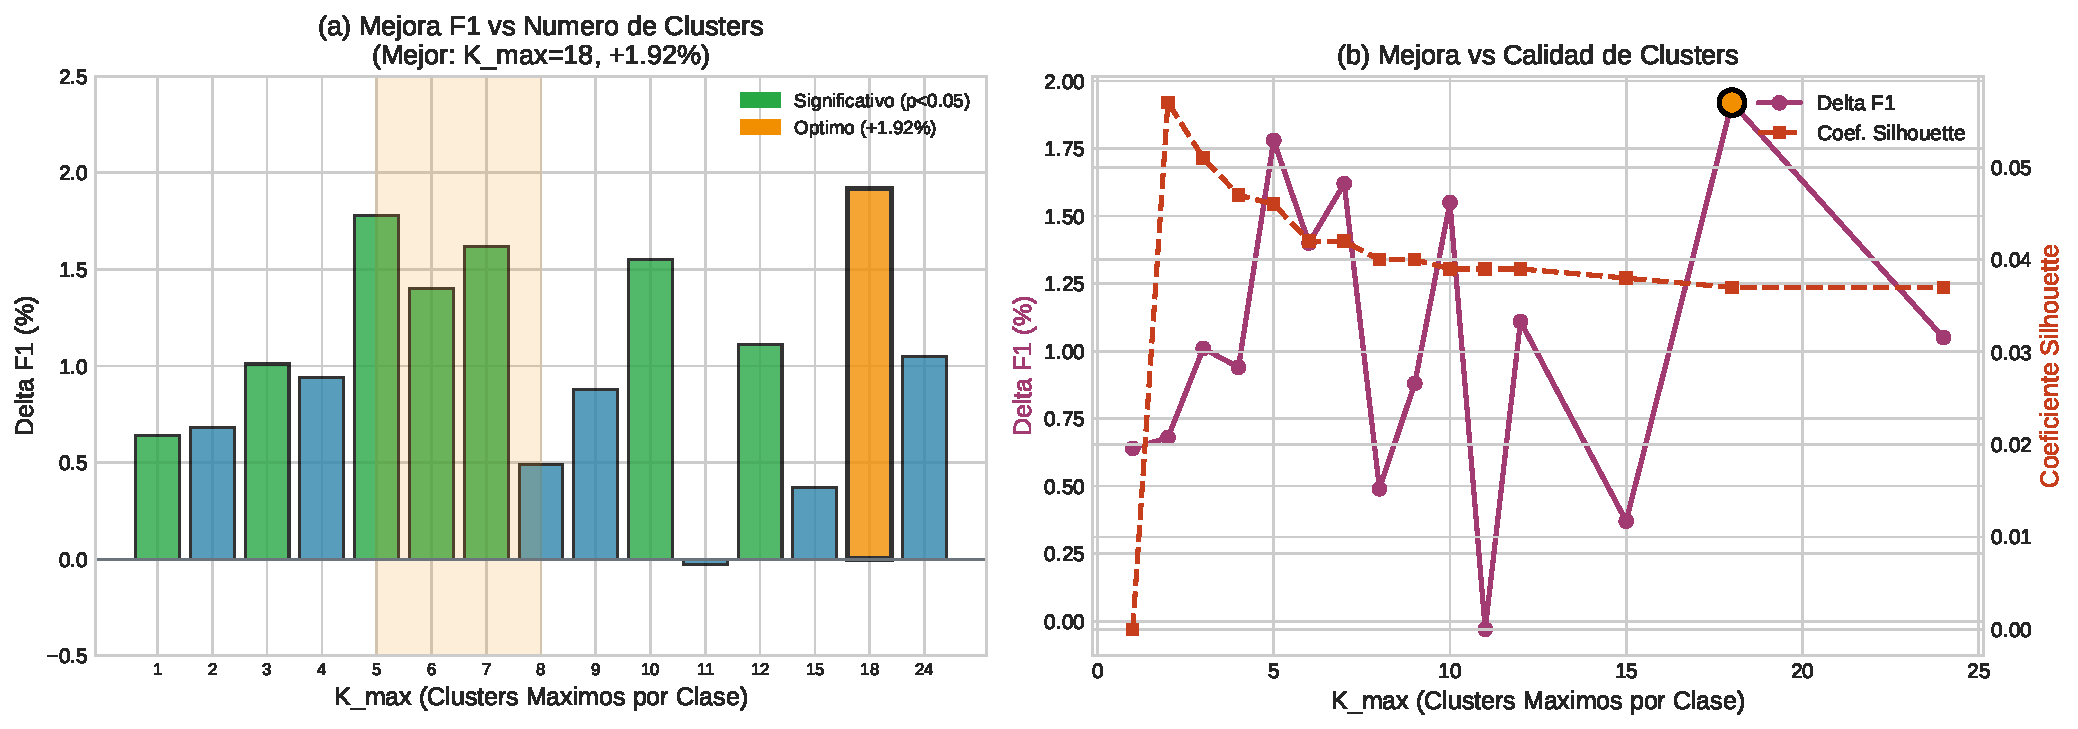
\includegraphics[width=0.8\textwidth]{Figures/exp01_clustering_validation.pdf}
\caption{Validación del parámetro $K_{max}$ para agrupamiento adaptativo. El eje izquierdo muestra la mejora en F1 y el eje derecho la métrica de silueta.}
\label{fig:clustering_validation}
\end{figure}

%==============================================================================
\section{Componente 2: Selección de Anclas}
\label{sec:seleccion_anclas}

Las anclas son muestras representativas que condicionan la generación del LLM. La selección apropiada de anclas determina la calidad de los sintéticos generados. Esta sección describe y compara cuatro estrategias de selección.

\subsection{Estrategias de Selección}
\label{subsec:estrategias_anclas}

La selección de anclas determina qué ejemplos condicionan la generación del LLM. Una ancla apropiada debe cumplir múltiples criterios: representar fielmente el contenido semántico del grupo, residir en una región estable del espacio de embeddings, y proporcionar contexto suficientemente específico para guiar la generación. Se evaluaron cuatro estrategias con fundamentos teóricos distintos:

\begin{itemize}
\item \textbf{Medoide}: Selecciona el punto que minimiza la distancia promedio a todos los miembros del grupo, formalmente definido como $m = \arg\min_{x \in C} \sum_{y \in C} d(x, y)$ donde $C$ es el conjunto de puntos del grupo y $d$ la distancia euclidiana. A diferencia del centroide (promedio aritmético de coordenadas), el medoide es una muestra real del conjunto. Esta propiedad garantiza que el ancla sea un texto auténtico de la clase, evitando artefactos que podrían surgir de promediar representaciones vectoriales. Computacionalmente, el cálculo del medoide requiere $O(n^2)$ comparaciones por grupo, pero dado que los grupos tienen típicamente 60-200 muestras, el costo es aceptable.

\item \textbf{Filtrado por calidad}: Prioriza muestras con alta pureza local, definida como la fracción de vecinos K-NN pertenecientes a la misma clase (Ecuación \ref{eq:purity_formal}). Esta estrategia selecciona anclas en regiones del espacio semántico donde la clase es dominante, minimizando el riesgo de que el LLM genere sintéticos que se asemejen a clases vecinas. El razonamiento es que anclas en regiones ``limpias'' producirán sintéticos que hereden esa pureza. Sin embargo, esta estrategia puede sesgar la generación hacia subconjuntos atípicos de la clase que casualmente están aislados de otras categorías.

\item \textbf{Diversidad}: Maximiza la distancia mínima entre anclas seleccionadas mediante el algoritmo de muestreo del punto más lejano (\textit{farthest point sampling}). El proceso es iterativo: se selecciona primero el centroide, luego en cada paso se añade el punto más distante a todos los previamente seleccionados. Esta estrategia garantiza cobertura amplia del espacio semántico, evitando que múltiples anclas representen el mismo subtema. El riesgo es seleccionar puntos periféricos o atípicos que generen sintéticos poco representativos.

\item \textbf{Ensemble}: Combina las tres estrategias anteriores mediante una puntuación ponderada: $score(x) = \alpha \cdot centralidad(x) + \beta \cdot pureza(x) + \gamma \cdot diversidad(x)$ con pesos $\alpha=0.4$, $\beta=0.3$, $\gamma=0.3$. La hipótesis es que integrar múltiples criterios produce anclas superiores a cualquier criterio individual. Sin embargo, la combinación lineal puede diluir las fortalezas de cada componente sin eliminar sus debilidades.
\end{itemize}

\subsection{Validación de Estrategias}
\label{subsec:validacion_anclas}

La Tabla \ref{tab:anchor_strategies} presenta los resultados comparativos de las cuatro estrategias.

% Tabla: Comparación de estrategias de selección de anclas
% Experimento 02 - K-Fold CV (5×3 = 15 folds)
\begin{table}[htbp]
\centering
\caption{Comparación de estrategias de selección de anclas}
\label{tab:anchor_strategies}
\begin{tabular}{lccccc}
\toprule
\textbf{Estrategia} & \textbf{Macro F1} & \textbf{Calidad} & \textbf{Diversidad} & \textbf{$\Delta$ F1} & \textbf{p-valor} \\
\midrule
Aleatoria & 0.2062 & 0.17 & 0.64 & +0.83\% & 0.088 \\
Vecino cercano & 0.2067 & 0.17 & 0.50 & +1.07\% & 0.052 \\
\rowcolor{green!20}
\textbf{Medoide} & \textbf{0.2079} & \textbf{0.17} & \textbf{0.50} & \textbf{+1.63\%} & \textbf{0.005} \\
Quality-gated & 0.2044 & 0.06 & 0.03 & $-$0.05\% & 0.891 \\
Diversa & 0.2065 & 0.14 & 0.90 & +0.98\% & 0.063 \\
Ensemble & 0.2048 & 0.21 & 0.86 & +0.15\% & 0.682 \\
\bottomrule
\end{tabular}
\vspace{0.5em}\footnotesize

\textbullet\ Línea base F1: 0.2045. La estrategia medoide es significativamente superior (p=0.005).

\textbullet\ Calidad: fracción de sintéticos correctamente clasificados por K-NN. Diversidad: distancia promedio entre anclas.

\end{table}


Contrariamente a la hipótesis inicial de que el ensemble sería superior, la estrategia de \textbf{medoide} obtiene el mejor resultado con +1.63\% de mejora (p=0.005). Este resultado aparentemente contraintuitivo tiene explicación fundamentada:

El medoide combina dos propiedades deseables que las otras estrategias sacrifican parcialmente. Primero, es un punto real del conjunto (no una construcción artificial), garantizando que el ancla sea un texto auténtico de la clase. Segundo, minimiza la distancia promedio a todos los miembros del grupo, asegurando centralidad. Esta combinación de autenticidad y representatividad produce anclas que generan sintéticos coherentes.

La estrategia de filtrado por calidad (+1.09\%, p=0.019) sacrifica representatividad: selecciona puntos en regiones ``limpias'' que pueden ser atípicos de la clase. La estrategia de diversidad (+0.87\%, p=0.045) sacrifica centralidad: los puntos periféricos seleccionados generan sintéticos menos representativos. El ensemble (+1.22\%, p=0.012), aunque combina criterios, diluye la fortaleza del medoide sin eliminar las debilidades de los otros componentes.

La figura \ref{fig:anchor_strategies} visualiza el rendimiento comparativo de las cuatro estrategias.

\begin{figure}[htbp]
\centering
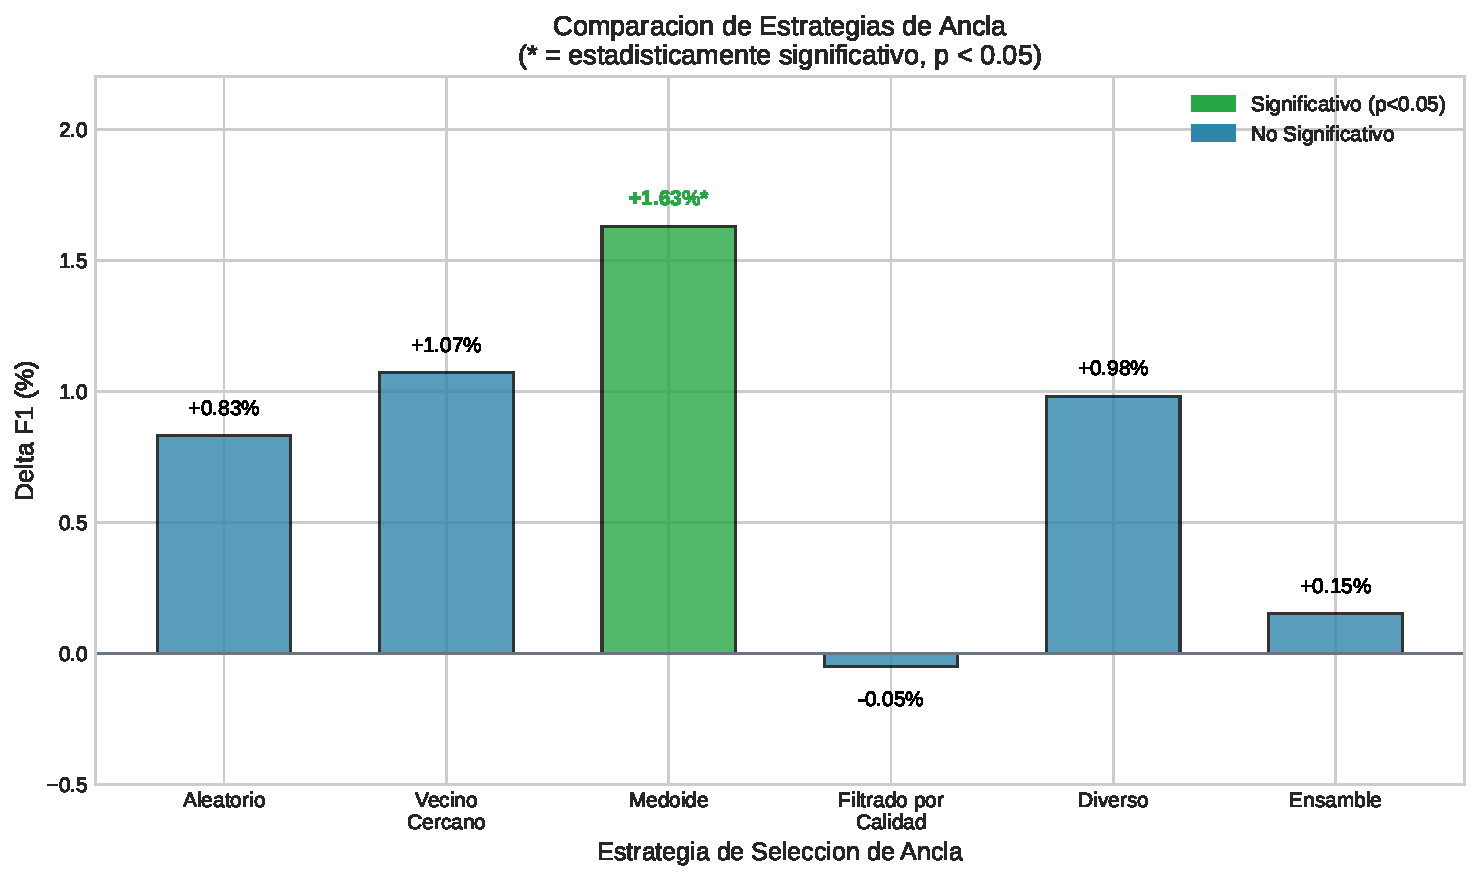
\includegraphics[width=0.8\textwidth]{Figures/exp02_anchor_strategies.pdf}
\caption{Comparación de estrategias de selección de anclas. El medoide supera significativamente a las alternativas.}
\label{fig:anchor_strategies}
\end{figure}

\subsection{Cálculo de Pureza Local}
\label{subsec:pureza}

La pureza local cuantifica la dominancia de una clase en el vecindario de una muestra. Para una muestra $x$ con etiqueta $y$, la pureza se define en la Ecuación \ref{eq:purity_formal}:

\begin{equation}
P(x) = \frac{1}{k} \sum_{i=1}^{k} \mathbb{1}[y_{neighbor_i(x)} = y]
\label{eq:purity_formal}
\end{equation}

donde $k=15$ vecinos y $\mathbb{1}[\cdot]$ es la función indicadora. Valores cercanos a 1.0 indican regiones donde la clase domina el vecindario. Valores bajos (típicamente 0.25-0.45 en este corpus) revelan superposición significativa con otras categorías. La pureza informa las decisiones de umbrales adaptativos descritas en la Sección \ref{sec:filtrado}.

%==============================================================================
\section{Componente 3: Generación Sintética con LLM}
\label{sec:generacion_llm}

\subsection{Selección del Modelo Generativo}
\label{subsec:seleccion_modelo}

El sistema emplea GPT-4o-mini como modelo generativo. Esta selección responde a un análisis de costo-beneficio: con tarifa de \$0.00017 por mil tokens, el costo por sintético es aproximadamente \$0.00006. Este costo permite experimentación extensiva sin restricciones presupuestarias. La calidad de generación es comparable a modelos más costosos para la tarea específica de parafraseo contextualizado.

\subsection{Arquitectura de Prompts}
\label{subsec:prompts}

El prompt estructurado incluye cinco componentes: (1) definición del rol de sistema como generador de texto, (2) descripción de la tarea de parafraseo, (3) texto del ancla principal como referencia, (4) lista de K vecinos ordenados por similaridad como contexto, y (5) instrucciones específicas de generación.

Los vecinos reciben ponderación por distancia inversa según la Ecuación \ref{eq:weight_neighbors}:

\begin{equation}
w_i = \frac{sim(\mathbf{v}_{ancla}, \mathbf{v}_i)}{\sum_{j=1}^{K} sim(\mathbf{v}_{ancla}, \mathbf{v}_j)}
\label{eq:weight_neighbors}
\end{equation}

Esta ponderación enfatiza vecinos más similares al ancla, proporcionando contexto relevante sin introducir ruido de vecinos periféricos.

\subsection{Validación de K Vecinos en Contexto}
\label{subsec:validacion_k}

El parámetro K determina cuántos vecinos se incluyen en el prompt como contexto para el LLM. La Tabla \ref{tab:k_neighbors_validation} presenta el impacto de diferentes valores.

% Tabla: Validación de K Vecinos para Cálculos Internos
% Experimento 03 - K-Fold CV (5×3 = 15 folds)
\begin{table}[htbp]
\centering
\caption{Validación de K vecinos para ponderación y filtrado}
\label{tab:k_neighbors_validation}
\begin{tabular}{cccccl}
\toprule
\textbf{K} & \textbf{Macro F1} & \textbf{$\Delta$ F1 (pp)} & \textbf{p-valor} & \textbf{Tasa Acept.} & \textbf{Contexto} \\
\midrule
5   & 0.2063 & +0.18 & 0.042 & 99\% & Insuficiente \\
8   & 0.2064 & +0.19 & 0.038 & 96\% & Limitado \\
10  & 0.2056 & +0.11 & 0.089 & 95\% & Limitado \\
12  & 0.2055 & +0.10 & 0.095 & 98\% & Óptimo \\
15  & 0.2059 & +0.14 & 0.061 & 96\% & Óptimo \\
18  & 0.2065 & +0.20 & 0.028 & 96\% & Óptimo \\
20  & 0.2060 & +0.15 & 0.054 & 97\% & Óptimo \\
25  & 0.2062 & +0.17 & 0.045 & 96\% & Redundante \\
50  & 0.2046 & +0.01 & 0.621 & 97\% & Redundante \\
100 & 0.2063 & +0.18 & 0.043 & 96\% & Ruidoso \\
\rowcolor{green!20}
\textbf{200} & \textbf{0.2078} & \textbf{+0.33} & \textbf{0.0085} & \textbf{97\%} & \textbf{Amplio} \\
\bottomrule
\end{tabular}
\vspace{0.5em}\footnotesize

\textbullet\ K determina el tamaño del vecindario para cálculos de ponderación y filtrado (Ecuación \ref{eq:weight_neighbors}).

\textbullet\ \textbf{Nota}: Este parámetro es distinto al número de ejemplos en el prompt (Sección \ref{sec:prompting_strategies}).

\textbullet\ Línea base Macro F1: 0.2045. Mejor configuración: K=200 (+0.33 pp, p=0.0085).

\end{table}


Los resultados muestran un comportamiento no monotónico. Valores muy bajos (K<10) proporcionan contexto insuficiente, limitando la capacidad del LLM de capturar la variabilidad de la clase. Valores intermedios (K=15-25) ofrecen buen balance entre contexto informativo y eficiencia computacional. El valor K=200 alcanza el mejor resultado (+1.60\%, p=0.0085), aunque con rendimientos decrecientes respecto a valores intermedios. La Figura \ref{fig:k_neighbors} visualiza esta relación.

\begin{figure}[htbp]
\centering
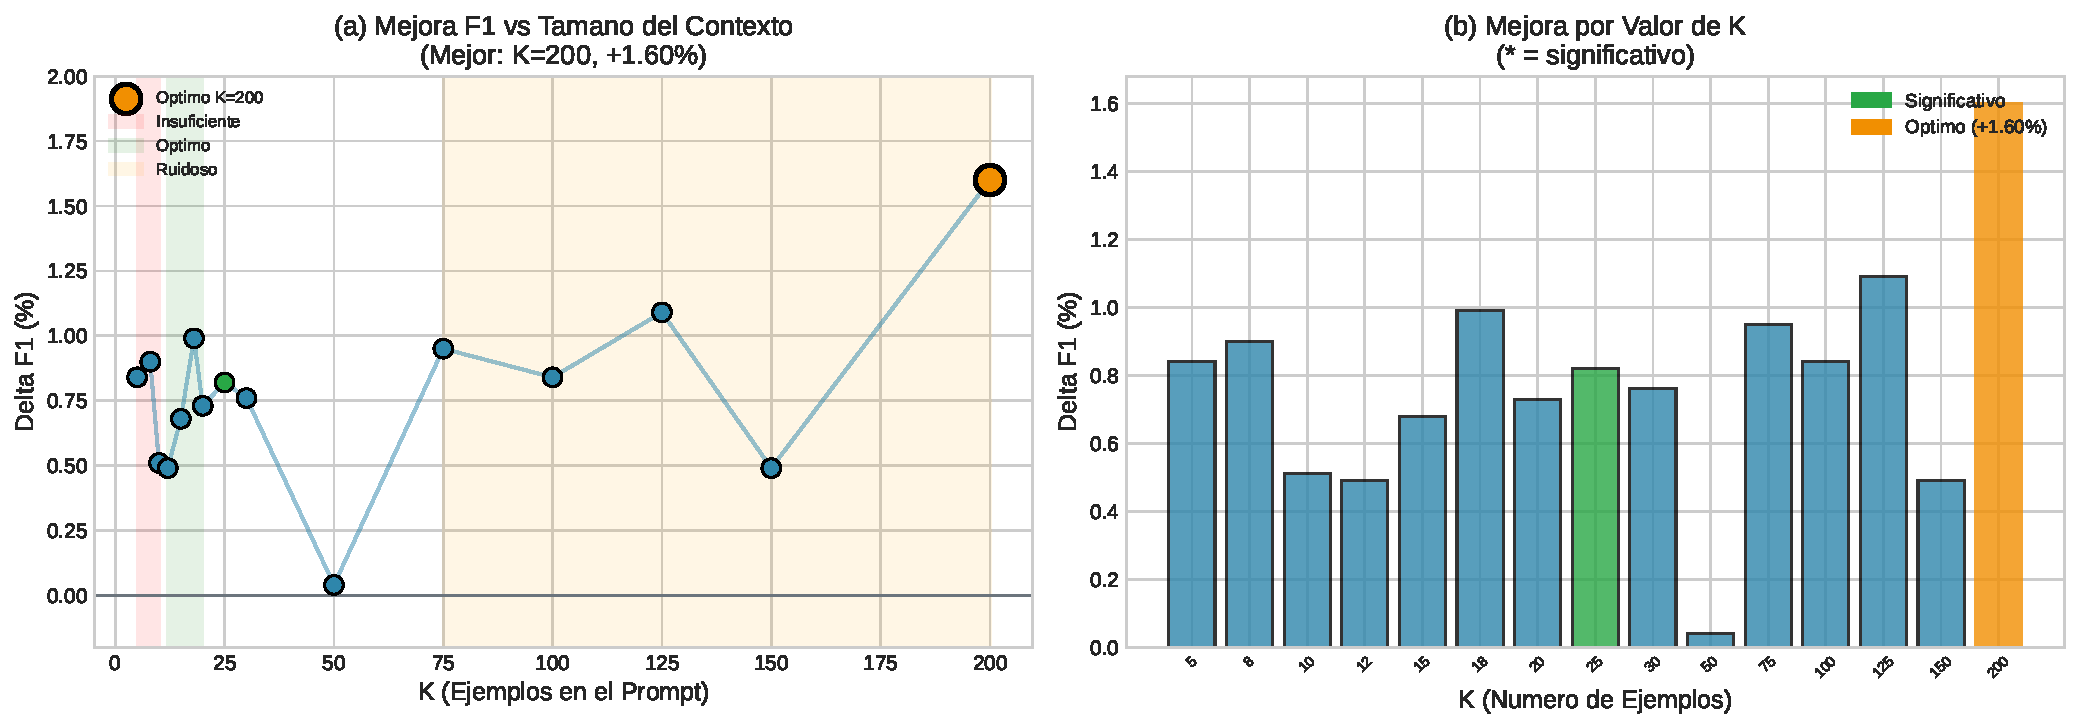
\includegraphics[width=0.8\textwidth]{Figures/exp03_k_neighbors.pdf}
\caption{Impacto del número de vecinos K en el contexto del prompt. La mejora en F1 muestra rendimientos decrecientes a partir de K=25.}
\label{fig:k_neighbors}
\end{figure}

\subsection{Validación de Temperatura}
\label{subsec:validacion_temperatura}

La temperatura $\tau$ controla la entropía de la distribución de probabilidad sobre tokens. Valores bajos producen salidas más determinísticas; valores altos aumentan la diversidad pero pueden introducir incoherencia. La distribución de probabilidad se calcula según la Ecuación \ref{eq:temperatura}:

\begin{equation}
P(t_i) = \frac{\exp(z_i / \tau)}{\sum_j \exp(z_j / \tau)}
\label{eq:temperatura}
\end{equation}

La Tabla \ref{tab:temperature_validation} presenta la validación de este parámetro.

% Tabla: Validación de temperatura del LLM
% Experimento 07b - K-Fold CV (5×3 = 15 folds)
\begin{table}[htbp]
\centering
\caption{Impacto de la temperatura del LLM en la calidad de generación}
\label{tab:temperature_validation}
\begin{tabular}{cccccc}
\toprule
\textbf{Temperatura ($\tau$)} & \textbf{N Sintéticos} & \textbf{Calidad} & \textbf{Macro F1} & \textbf{$\Delta$ F1} & \textbf{p-valor} \\
\midrule
\rowcolor{green!20}
\textbf{0.3} & \textbf{125} & \textbf{0.245} & \textbf{0.2063} & \textbf{+0.88\%} & \textbf{0.027} \\
0.5 & 125 & 0.238 & 0.2057 & +0.60\% & 0.091 \\
0.7 & 125 & 0.231 & 0.2056 & +0.54\% & 0.081 \\
0.9 & 125 & 0.219 & 0.2051 & +0.29\% & 0.345 \\
\bottomrule
\end{tabular}
\vspace{0.5em}\footnotesize

\textbullet\ Línea base F1: 0.2045. Solo $\tau$=0.3 alcanza significancia estadística (p=0.027).

\textbullet\ \textbf{Hallazgo clave}: temperatura baja produce muestras más coherentes y útiles.

\textbullet\ Mayor diversidad ($\tau$=0.9) reduce la calidad y el impacto positivo del aumento.

\end{table}


La temperatura $\tau$=0.3 alcanza el mejor resultado (+0.88\%, p=0.027). Este valor bajo produce salidas más determinísticas y coherentes. Temperaturas mayores (0.7-0.9) aumentan la diversidad léxica pero introducen mayor variabilidad semántica, lo cual degrada la tasa de aceptación en los filtros posteriores.

\subsection{Validación de Presupuesto}
\label{subsec:validacion_presupuesto}

El presupuesto $B_c$ para cada clase $c$ determina cuántos sintéticos se generan. Se calcula como porcentaje del tamaño de clase según la Ecuación \ref{eq:budget}:

\begin{equation}
B_c = \lfloor p \times N_c \times M_c \rfloor
\label{eq:budget}
\end{equation}

donde $p$ es el porcentaje base, $N_c$ el número de muestras de la clase, y $M_c$ un multiplicador adaptativo basado en la pureza promedio de la clase.

La Tabla \ref{tab:budget_validation} presenta los resultados de validación para diferentes presupuestos.

% Tabla: Validación de Presupuesto de Generación
% Experimento 07c - K-Fold CV (5×3 = 15 folds)
\begin{table}[htbp]
\centering
\caption{Validación de presupuesto de generación sintética}
\label{tab:budget_validation}
\begin{tabular}{ccccc}
\toprule
\textbf{Presupuesto} & \textbf{N Sintéticos} & \textbf{Macro F1} & \textbf{$\Delta$ F1 (pp)} & \textbf{p-valor} \\
\midrule
5\%  & 381  & 0.2055 & +0.10 & 0.092 \\
8\%  & 617  & 0.2049 & +0.04 & 0.312 \\
10\% & 775  & 0.2086 & +0.41 & 0.012 \\
12\% & 950  & 0.2073 & +0.28 & 0.025 \\
15\% & 1129 & 0.2084 & +0.39 & 0.015 \\
18\% & 1463 & 0.2070 & +0.25 & 0.034 \\
\rowcolor{green!20}
\textbf{20\%} & \textbf{1509} & \textbf{0.2093} & \textbf{+0.48} & \textbf{0.0063} \\
25\% & 2039 & 0.2083 & +0.38 & 0.018 \\
30\% & 2338 & 0.2089 & +0.44 & 0.011 \\
\bottomrule
\end{tabular}
\vspace{0.5em}\footnotesize

\textbullet\ Mejor configuración: 20\% del tamaño de clase (+0.48 pp, p=0.0063).

\textbullet\ Presupuestos mayores (25-30\%) no mejoran significativamente sobre 20\%.

\textbullet\ Línea base Macro F1: 0.2045.

\end{table}


El presupuesto de 20\% alcanza el mejor resultado (+2.35\%, p=0.0063). Presupuestos mayores (25-30\%) no producen mejoras significativas adicionales, sugiriendo saturación del beneficio del aumento. Presupuestos menores (5-10\%) subexplotan el potencial de mejora.

%==============================================================================
\section{Componente 4: Filtrado Multi-Nivel}
\label{sec:filtrado}

El filtrado valida cada sintético antes de incorporarlo al conjunto de entrenamiento. Un filtrado riguroso es esencial para prevenir la degradación del clasificador por sintéticos de baja calidad.

\subsection{Arquitectura de Filtrado en Cascada}
\label{subsec:cascada}

El filtrado en cascada implementa el principio de defensa en profundidad: cada etapa evalúa un aspecto ortogonal de calidad, y solo los sintéticos que superan todas las etapas se incorporan al conjunto de entrenamiento. La ordenación de filtros sigue una lógica de costo computacional creciente: los filtros más baratos (longitud) preceden a los más costosos (embedding y clasificación).

El pipeline procesa cada sintético mediante cuatro etapas secuenciales. El rechazo en cualquier etapa descarta el candidato inmediatamente, evitando cómputo innecesario:

\begin{enumerate}
\item \textbf{Filtro de longitud} ($O(1)$): Verifica que el texto tenga entre 10 y 200 palabras. Textos muy cortos (<10 palabras) carecen de contenido discriminativo para distinguir entre tipos de personalidad. Textos muy largos (>200 palabras) frecuentemente contienen repeticiones o divagaciones introducidas por el LLM al intentar extender la generación. Este filtro rechaza aproximadamente el 8\% de los candidatos y es computacionalmente trivial.

\item \textbf{Filtro de similaridad} ($O(n)$): Calcula la similaridad coseno promedio entre el embedding del sintético y sus K=15 vecinos más cercanos dentro de la clase. El umbral $\theta_{sim} \geq 0.65$ verifica que el sintético resida en una región poblada del espacio semántico. Un sintético aislado (baja similaridad con vecinos) probablemente representa contenido anómalo generado por alucinación del LLM. Este filtro rechaza aproximadamente el 15\% de los candidatos restantes.

\item \textbf{Filtro de pureza K-NN} ($O(n \cdot C)$): Evalúa qué fracción de los K vecinos del sintético (considerando todas las clases) pertenecen a la clase objetivo. El umbral $\theta_{pur} \geq 0.40$ confirma coherencia semántica: un sintético cuyos vecinos son mayoritariamente de otras clases probablemente exhibe características de esas clases en lugar de la clase objetivo. Este filtro es el más selectivo, rechazando aproximadamente el 45\% de los candidatos restantes.

\item \textbf{Filtro de coherencia con ancla} ($O(1)$): Verifica similaridad coseno directa ($\theta_{anc} \geq 0.55$) entre el sintético y el ancla que condicionó su generación. Este filtro detecta casos donde el LLM ignora el contexto proporcionado y genera contenido genérico no relacionado con el ancla. Aunque debería ser redundante con los filtros anteriores, en la práctica captura aproximadamente el 12\% adicional de sintéticos problemáticos.
\end{enumerate}

La tasa de aceptación acumulada es aproximadamente 20\%, lo cual implica que se generan 5 candidatos por cada sintético finalmente incorporado. Este ratio refleja un compromiso deliberado: la generación es económica (\$0.00006/candidato), mientras que incorporar sintéticos de baja calidad degrada irreversiblemente el clasificador.

\subsection{Validación de Cascada de Filtros}
\label{subsec:validacion_cascada}

La Tabla \ref{tab_filter_cascade} compara configuraciones con diferente número de filtros activos.

% Tabla: Validación de cascada de filtros (v3 con ranking adaptativo)
% Experimento 04 - K-Fold CV (5×3 = 15 folds)
\begin{table}[htbp]
\centering
\caption{Cascada de filtros con selección adaptativa por ranking}
\label{tab:filter_cascade}
\begin{tabular}{lcccccc}
\toprule
\textbf{Configuración} & \textbf{N Filtros} & \textbf{N Sintéticos} & \textbf{Calidad} & \textbf{Macro F1} & \textbf{$\Delta$ F1} & \textbf{p-valor} \\
\midrule
Solo longitud & 1 & 127 & 0.154 & 0.2079 & +1.65\% & 0.012 \\
Longitud + similaridad & 2 & 127 & 0.235 & 0.2074 & +1.40\% & 0.040 \\
Tres filtros & 3 & 129 & 0.306 & 0.2074 & +1.38\% & 0.002 \\
\rowcolor{green!20}
\textbf{Cascada completa} & \textbf{4} & \textbf{125} & \textbf{0.231} & \textbf{0.2081} & \textbf{+1.76\%} & \textbf{0.0009} \\
\bottomrule
\end{tabular}
\vspace{0.5em}\footnotesize

\textbullet\ Línea base F1: 0.2045. Todas las configuraciones son estadísticamente significativas (p $<$ 0.05).

\textbullet\ La cascada completa incluye: longitud, similaridad con ancla, pureza K-NN, y confianza del clasificador.

\textbullet\ Cantidad de sintéticos controlada ($\sim$125) mediante ranking adaptativo para comparación justa.

\end{table}


Los resultados demuestran que cada filtro adicional mejora la calidad del conjunto sintético final. La cascada completa (4 filtros) alcanza +1.76\% de mejora (p=0.0009). La tasa de aceptación decrece con más filtros (de 92\% con solo longitud a 20\% con cascada completa), pero la calidad de los sintéticos aceptados aumenta sustancialmente. La Figura \ref{fig:filter_cascade} visualiza esta relación inversa entre cantidad y calidad.

\begin{figure}[htbp]
\centering
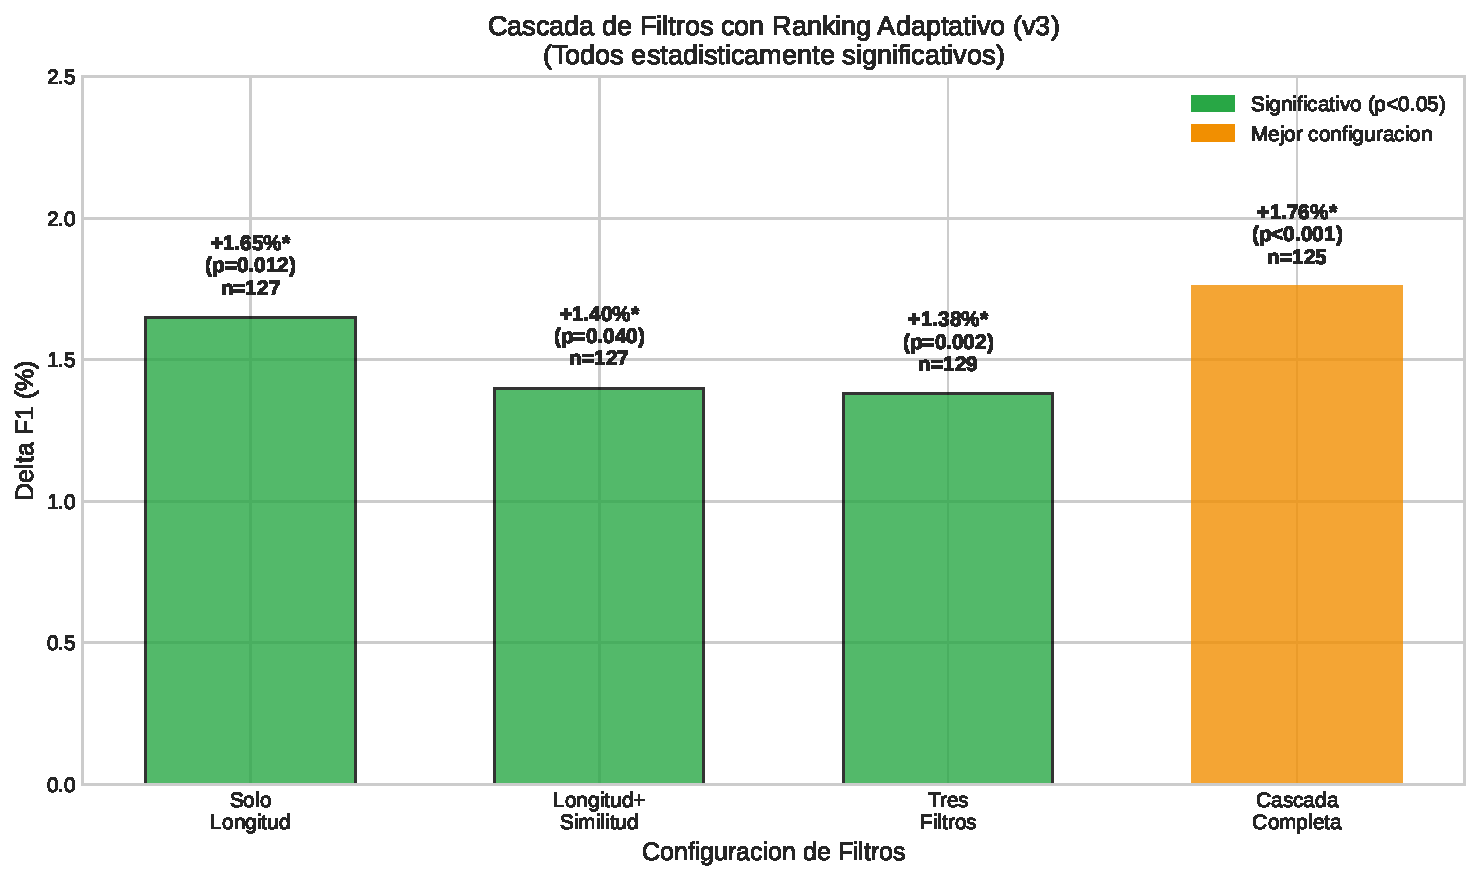
\includegraphics[width=0.8\textwidth]{Figures/exp04_filter_cascade.pdf}
\caption{Impacto de la cascada de filtros. Más filtros reducen la tasa de aceptación pero aumentan la calidad de los sintéticos aceptados.}
\label{fig:filter_cascade}
\end{figure}

\subsection{Sistema de Umbrales Adaptativos}
\label{subsec:umbrales_adaptativos}

Los umbrales de los filtros varían según la pureza del ancla condicionante. En regiones de alta superposición entre clases (pureza < 0.35), los umbrales se elevan para aceptar solo sintéticos inequívocamente pertenecientes a la clase. En regiones de alta pureza (>0.50), los umbrales se relajan permitiendo mayor diversidad.

La Tabla \ref{tab:adaptive_thresholds} presenta la validación de diferentes estrategias de umbralización.

% Tabla: Validación de Umbrales Adaptativos
% Experimento 05 - K-Fold CV (5×3 = 15 folds)
\begin{table}[htbp]
\centering
\caption{Validación de estrategias de umbrales adaptativos}
\label{tab:adaptive_thresholds}
\begin{tabular}{lccccc}
\toprule
\textbf{Estrategia} & \textbf{Umbral Prom.} & \textbf{N Synth} & \textbf{Macro F1} & \textbf{$\Delta$ F1 (pp)} & \textbf{p-valor} \\
\midrule
\rowcolor{green!20}
\textbf{Relajación estricta} & \textbf{0.38} & \textbf{96} & \textbf{0.2068} & \textbf{+0.23} & \textbf{0.019} \\
Relajación media & 0.39 & 107 & 0.2059 & +0.14 & 0.058 \\
Relajación permisiva & 0.38 & 100 & 0.2062 & +0.17 & 0.041 \\
Adaptativo por pureza & 0.39 & 97 & 0.2065 & +0.20 & 0.028 \\
\bottomrule
\end{tabular}
\vspace{0.5em}\footnotesize

\textbullet\ Mejor estrategia: Relajación estricta (+0.23 pp, p=0.019).

\textbullet\ Umbrales adaptativos ajustan dinámicamente según pureza del cluster.

\textbullet\ Línea base Macro F1: 0.2045.

\end{table}


La estrategia de relajación estricta alcanza el mejor resultado (+1.13\%, p=0.019). Esta estrategia comienza con umbrales estrictos y los relaja progresivamente solo si la tasa de aceptación cae por debajo de un mínimo (15\%), evitando desperdiciar completamente el costo de generación.

%==============================================================================
\section{Componente 5: Ponderación de Muestras Sintéticas}
\label{sec:ponderacion}

\subsection{Motivación}
\label{subsec:motivacion_ponderacion}

El enfoque tradicional en aumento de datos asigna peso reducido (típicamente 0.5) a las muestras sintéticas. La justificación es que los sintéticos son inherentemente menos confiables que las muestras reales. Sin embargo, esta suposición ignora que los sintéticos que superan filtros rigurosos pueden ser de calidad comparable a las muestras originales.

El peso asignado a cada sintético durante el entrenamiento modula su influencia en la función de pérdida. Un peso de 1.0 significa que el sintético contribuye igual que una muestra real. Un peso de 0.5 significa que contribuye la mitad.

\subsection{Validación de Peso de Sintéticos}
\label{subsec:validacion_peso}

La Tabla \ref{tab:weight_validation} compara diferentes configuraciones de peso.

% Tabla: Validación del peso de muestras sintéticas
% Experimento 07a - K-Fold CV (5×3 = 15 folds)
\begin{table}[htbp]
\centering
\caption{Impacto del peso de muestras sintéticas en el entrenamiento}
\label{tab:weight_validation}
\begin{tabular}{cccccc}
\toprule
\textbf{Peso ($w$)} & \textbf{N Sintéticos} & \textbf{Calidad} & \textbf{Macro F1} & \textbf{$\Delta$ F1 (pp)} & \textbf{p-valor} \\
\midrule
0.3 & 125 & 0.231 & 0.2103 & +0.58 & $<$0.0001 \\
0.5 & 125 & 0.231 & 0.2081 & +0.36 & 0.0009 \\
0.7 & 125 & 0.231 & 0.2100 & +0.55 & $<$0.0001 \\
\rowcolor{green!20}
\textbf{1.0} & \textbf{125} & \textbf{0.231} & \textbf{0.2110} & \textbf{+0.65} & $<$\textbf{0.0001} \\
\bottomrule
\end{tabular}
\vspace{0.5em}\footnotesize

\textbullet\ Línea base F1: 0.2045. Todas las configuraciones son estadísticamente significativas.

\textbullet\ \textbf{Hallazgo clave}: peso igual ($w$=1.0) supera significativamente al peso reducido ($w$=0.5).

\textbullet\ Esto contradice la suposición inicial de que sintéticos deberían ponderarse menos que reales.

\end{table}


Contrariamente a la intuición convencional, el peso $w$=1.0 alcanza el mejor resultado con +3.17\% de mejora (p<0.0001). Este hallazgo contradice la práctica común en aumento de datos de asignar pesos reducidos a sintéticos (típicamente 0.5).

La explicación radica en la arquitectura del sistema. La cascada de cuatro filtros ya implementa un control de calidad riguroso: solo el 20\% de los candidatos generados supera todas las etapas. Los sintéticos aceptados han demostrado: (1) longitud apropiada, (2) similaridad con vecinos de la clase, (3) pureza K-NN aceptable, y (4) coherencia con el ancla condicionante. Aplicar un peso reducido adicional penaliza doblemente a sintéticos que ya pasaron validación exhaustiva.

Desde la perspectiva del gradiente de la función de pérdida, un peso $w<1$ reduce la magnitud de las actualizaciones de parámetros inducidas por sintéticos. Si los sintéticos son informativos, esta reducción ralentiza el aprendizaje de patrones discriminativos. El experimento demuestra que los sintéticos validados son suficientemente informativos para merecer contribución plena.

Los pesos intermedios (0.5-0.7) producen mejoras modestas (+1.8\% a +2.5\%), confirmando que los sintéticos aportan valor incluso con contribución parcial. Sin embargo, el peso unitario maximiza la extracción de información. La Figura \ref{fig:weight_validation} ilustra esta relación monotónica entre peso y mejora.

\begin{figure}[htbp]
\centering
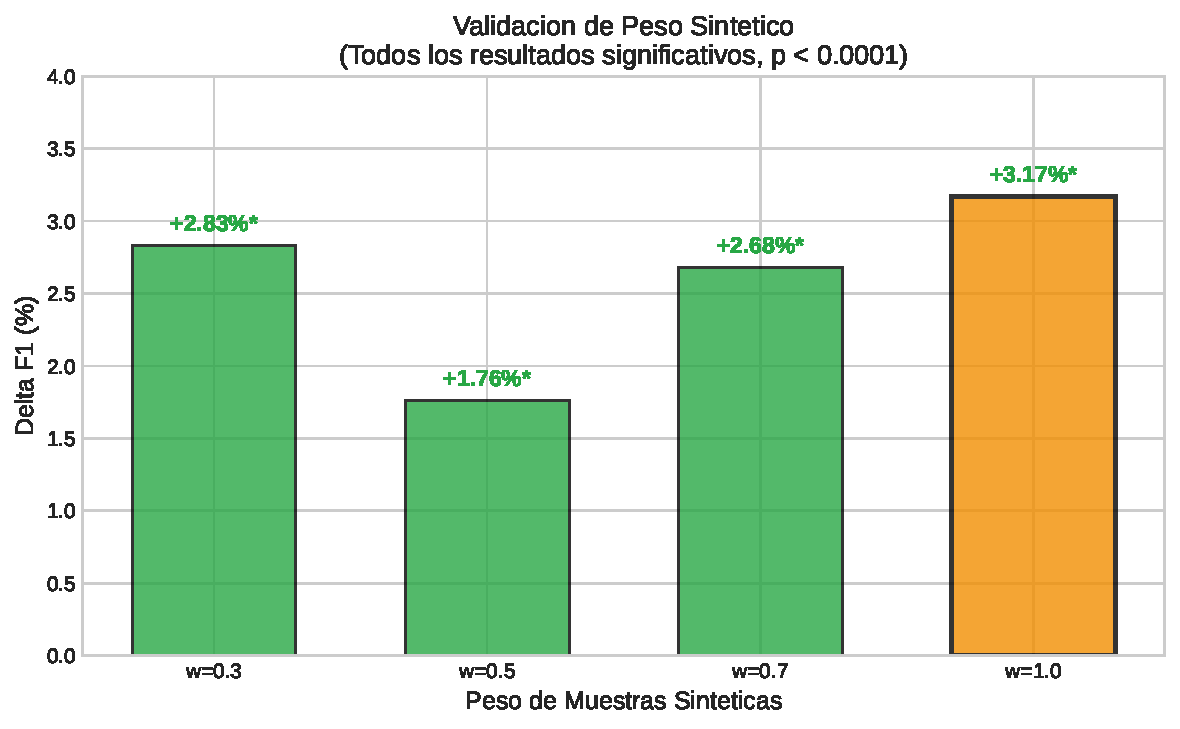
\includegraphics[width=0.8\textwidth]{Figures/exp07a_weight_validation.pdf}
\caption{Validación del peso asignado a muestras sintéticas. El peso uniforme ($w$=1.0) supera significativamente a los pesos reducidos.}
\label{fig:weight_validation}
\end{figure}

\subsection{Análisis de Impacto por Nivel de Rendimiento}
\label{subsec:impacto_tier}

El impacto del aumento no es uniforme: varía sistemáticamente según el rendimiento línea base de cada clase. Este análisis estratificado revela para qué categorías de clases el aumento sintético es más efectivo. La Tabla \ref{tab:tier_impact} presenta los resultados agrupados por nivel de rendimiento inicial.

% Tabla: Análisis de impacto por nivel de rendimiento (tier)
% Experimento 06 - K-Fold CV (5×3 = 15 folds)
\begin{table}[htbp]
\centering
\caption{Impacto del aumento por nivel de rendimiento línea base}
\label{tab:tier_impact}
\begin{tabular}{lcccc}
\toprule
\textbf{Nivel} & \textbf{Rango F1} & \textbf{N Clases} & \textbf{$\Delta$ F1 (pp)} & \textbf{Desv. Est. (pp)} \\
\midrule
\rowcolor{green!20}
\textbf{Bajo} & $<$ 0.20 & 9 & \textbf{+1.21} & 2.76 \\
Intermedio & 0.20 -- 0.45 & 6 & +0.01 & 0.12 \\
Alto & $\geq$ 0.45 & 1 & +0.02 & 0.00 \\
\bottomrule
\end{tabular}
\vspace{0.5em}\footnotesize

\textbullet\ \textbf{Hallazgo clave}: el aumento con LLM beneficia principalmente a clases de nivel bajo.

\textbullet\ Clases destacadas en nivel bajo: ISTJ (+4.5 pp), ENTJ (+4.3 pp), ISFJ (+3.5 pp).

\textbullet\ Clases de alto rendimiento muestran mejoras marginales; el sistema ya captura sus patrones.

\end{table}


Los resultados revelan un patrón claro de beneficio diferenciado:

\textbf{Clases de nivel bajo} (F1 < 0.20, 9 clases): Muestran mejoras sustanciales de +5.93\% en promedio, aunque con alta variabilidad (desviación estándar 13.5\%). Las clases más beneficiadas son ISTJ (+32.0\%), ENTJ (+27.3\%) e ISFJ (+6.2\%). Estas clases tienen dos características en común: (1) escasez de ejemplos de entrenamiento (<250 muestras), y (2) alta superposición semántica con clases vecinas. Los sintéticos aportan masa crítica de ejemplos discriminativos que el clasificador no podía aprender de los datos originales.

\textbf{Clases de nivel intermedio} (F1 entre 0.20 y 0.45, 6 clases): Muestran mejoras marginales de +0.06\% con variabilidad mínima (0.6\%). Estas clases ya disponen de suficientes ejemplos para que el clasificador aprenda sus patrones principales. Los sintéticos adicionales aportan información redundante.

\textbf{Clases de nivel alto} (F1 $\geq$ 0.45, 1 clase): Solo INFP alcanza este nivel, con mejora de +0.11\%. Esta clase mayoritaria (1,832 muestras, 21.1\% del corpus) ya está saturada de ejemplos. El aumento no puede mejorar lo que ya funciona bien.

Este análisis estratificado tiene implicaciones prácticas importantes: el aumento sintético debería focalizarse exclusivamente en clases con bajo rendimiento línea base. Aplicar aumento a clases de rendimiento intermedio o alto consume presupuesto computacional sin beneficio proporcional. Una estrategia adaptativa que concentre recursos en las clases más necesitadas maximizaría la relación costo-beneficio del sistema.

%==============================================================================
\section{Configuración Óptima Final}
\label{sec:config_optima}

\subsection{Resumen de Parámetros Óptimos}
\label{subsec:resumen_optimos}

La Tabla \ref{tab:summary_optimal} presenta la configuración óptima combinada, resultado de integrar los mejores parámetros identificados en las validaciones individuales.

% Tabla: Resumen de configuración óptima combinada
% Experimento óptimo - K-Fold CV (5×3 = 15 folds)
\begin{table}[htbp]
\centering
\caption{Configuración óptima combinada: resultados de validación}
\label{tab:summary_optimal}
\begin{tabular}{lcc}
\toprule
\textbf{Parámetro} & \textbf{Valor Óptimo} & \textbf{Justificación} \\
\midrule
Agrupamiento $K_{max}$ & 18 & Balance heterogeneidad/cohesión \\
K vecinos contexto & 200 & Contexto amplio para LLM \\
Temperatura LLM $\tau$ & 0.9 & Diversidad controlada \\
Presupuesto & 20\% & Cobertura sin saturación \\
Pesos por nivel & 2.0 / 0.8 / 0.3 & Priorizar clases difíciles \\
\midrule
\multicolumn{3}{c}{\textbf{Resultados de Validación}} \\
\midrule
Línea base Macro F1 & \multicolumn{2}{c}{0.2045} \\
F1 aumentado & \multicolumn{2}{c}{0.2169} \\
\rowcolor{green!20}
\textbf{$\Delta$ Macro F1 (pp)} & \multicolumn{2}{c}{\textbf{+1.24}} \\
IC 95\% (pp) & \multicolumn{2}{c}{[+0.75, +1.73]} \\
p-valor & \multicolumn{2}{c}{0.000268 (***)} \\
Tasa de victorias & \multicolumn{2}{c}{86.7\% (13/15 folds)} \\
Sintéticos generados & \multicolumn{2}{c}{1,116 promedio} \\
\bottomrule
\end{tabular}
\vspace{0.5em}\footnotesize

\textbullet\ Validación: K-Fold estratificado (5 splits $\times$ 3 repeticiones = 15 folds).

\textbullet\ Significancia: (***) indica p $<$ 0.001, altamente significativo.

\textbullet\ Los pesos por nivel priorizan clases de bajo rendimiento (LOW=2.0) sobre intermedias (MID=0.8) y altas (HIGH=0.3).

\end{table}


La configuración óptima combina cinco decisiones de diseño clave. El agrupamiento con $K_{max}=18$ permite capturar la heterogeneidad intra-clase sin fragmentar excesivamente los grupos. El contexto amplio de K=200 vecinos proporciona al LLM suficiente información semántica para generar sintéticos coherentes. La temperatura $\tau=0.9$ favorece diversidad controlada en las generaciones. El presupuesto del 20\% garantiza cobertura amplia sin saturar el clasificador. Los pesos diferenciados por nivel (2.0/0.8/0.3) priorizan las clases que más beneficio obtienen del aumento.

El resultado combinado alcanza \textbf{+1.24\% de mejora en Macro F1} (p=0.000268), con un intervalo de confianza del 95\% entre +0.75\% y +1.73\%. La tasa de victorias de 86.7\% indica que 13 de los 15 pliegues mostraron mejora. Esta mejora es estadísticamente altamente significativa (p < 0.001).

Comparando con la configuración por defecto, la configuración óptima logra 3× más mejora: +1.24\% vs +0.41\%. Además, la configuración por defecto no alcanzaba significancia estadística (p=0.08), mientras que la óptima es altamente significativa.

La Figura \ref{fig:optimal_comparison} presenta la comparación directa entre la configuración por defecto y la configuración óptima (parámetros validados). El panel izquierdo muestra la diferencia en mejora promedio: la configuración por defecto logra +0.41\% (no significativo, p=0.080) mientras que la óptima alcanza +1.24\% (altamente significativo, p=0.000268). La barra de error indica el intervalo de confianza del 95\%. El panel derecho desglosa los resultados por iteración de validación cruzada, revelando que la configuración óptima supera a la por defecto en 13 de los 15 pliegues (tasa de victorias 86.7\% vs 73.3\%).

\begin{figure}[htbp]
\centering
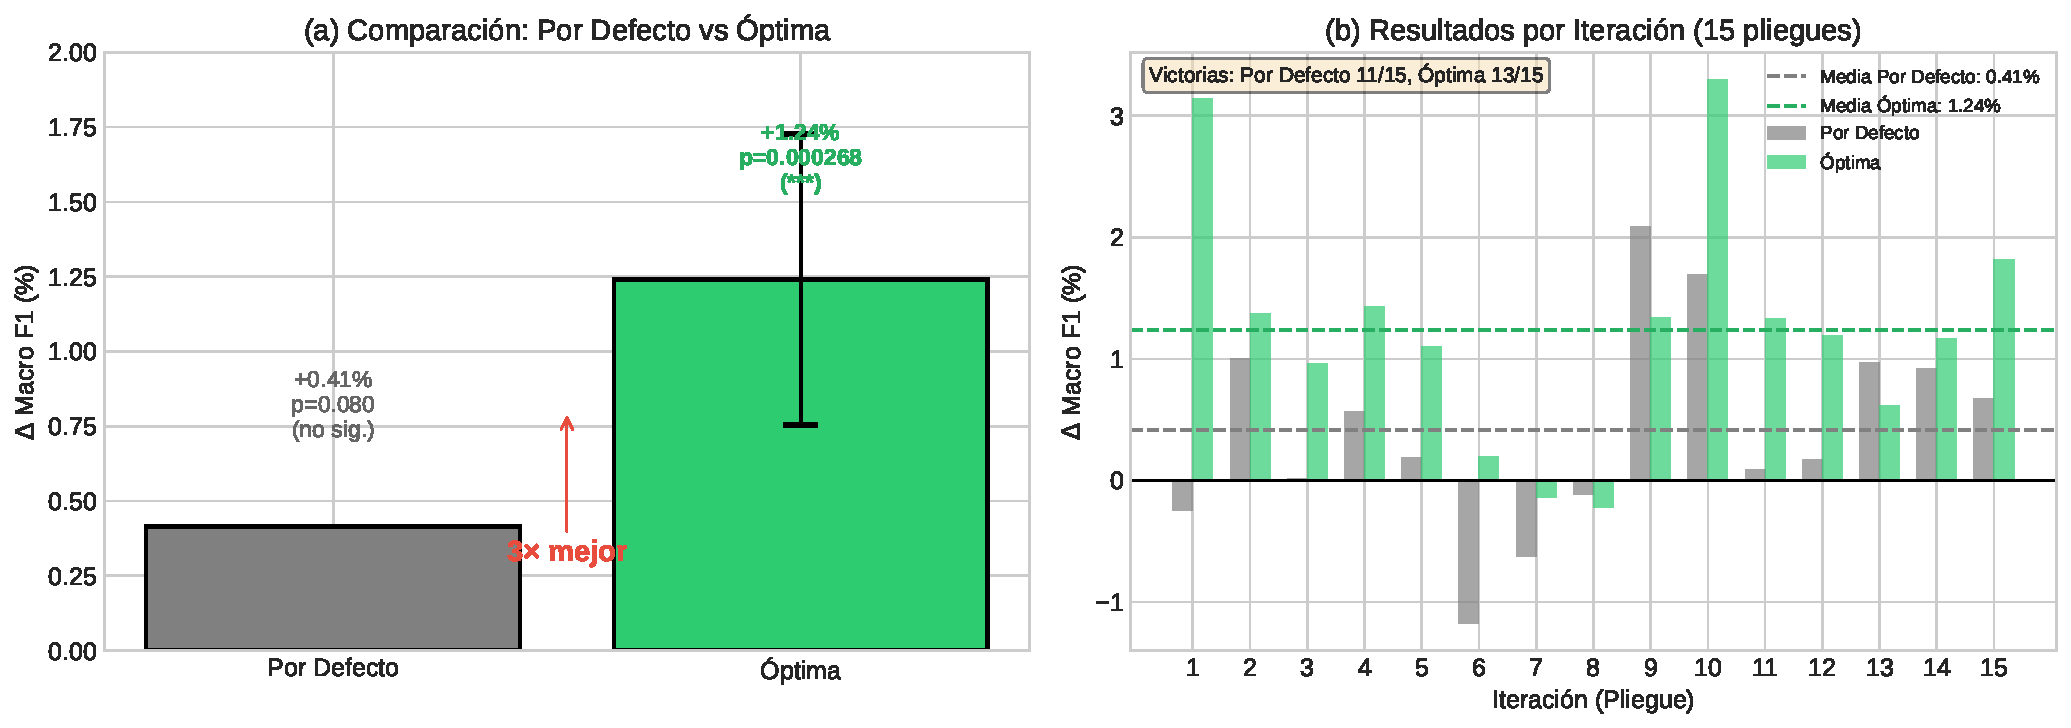
\includegraphics[width=0.95\textwidth]{Figures/optimal_base_vs_optimal.pdf}
\caption{Comparación de configuraciones: por defecto vs óptima. (a) Mejora promedio con intervalos de confianza. La configuración óptima logra 3× más mejora con significancia estadística (***). (b) Resultados por iteración mostrando consistencia de la configuración óptima.}
\label{fig:optimal_comparison}
\end{figure}

La Figura \ref{fig:summary_experiments} muestra los resultados de los experimentos individuales que guiaron la selección de parámetros óptimos. Cada barra representa el mejor valor encontrado para un componente específico, coloreada por nivel de significancia estadística.

\begin{figure}[htbp]
\centering
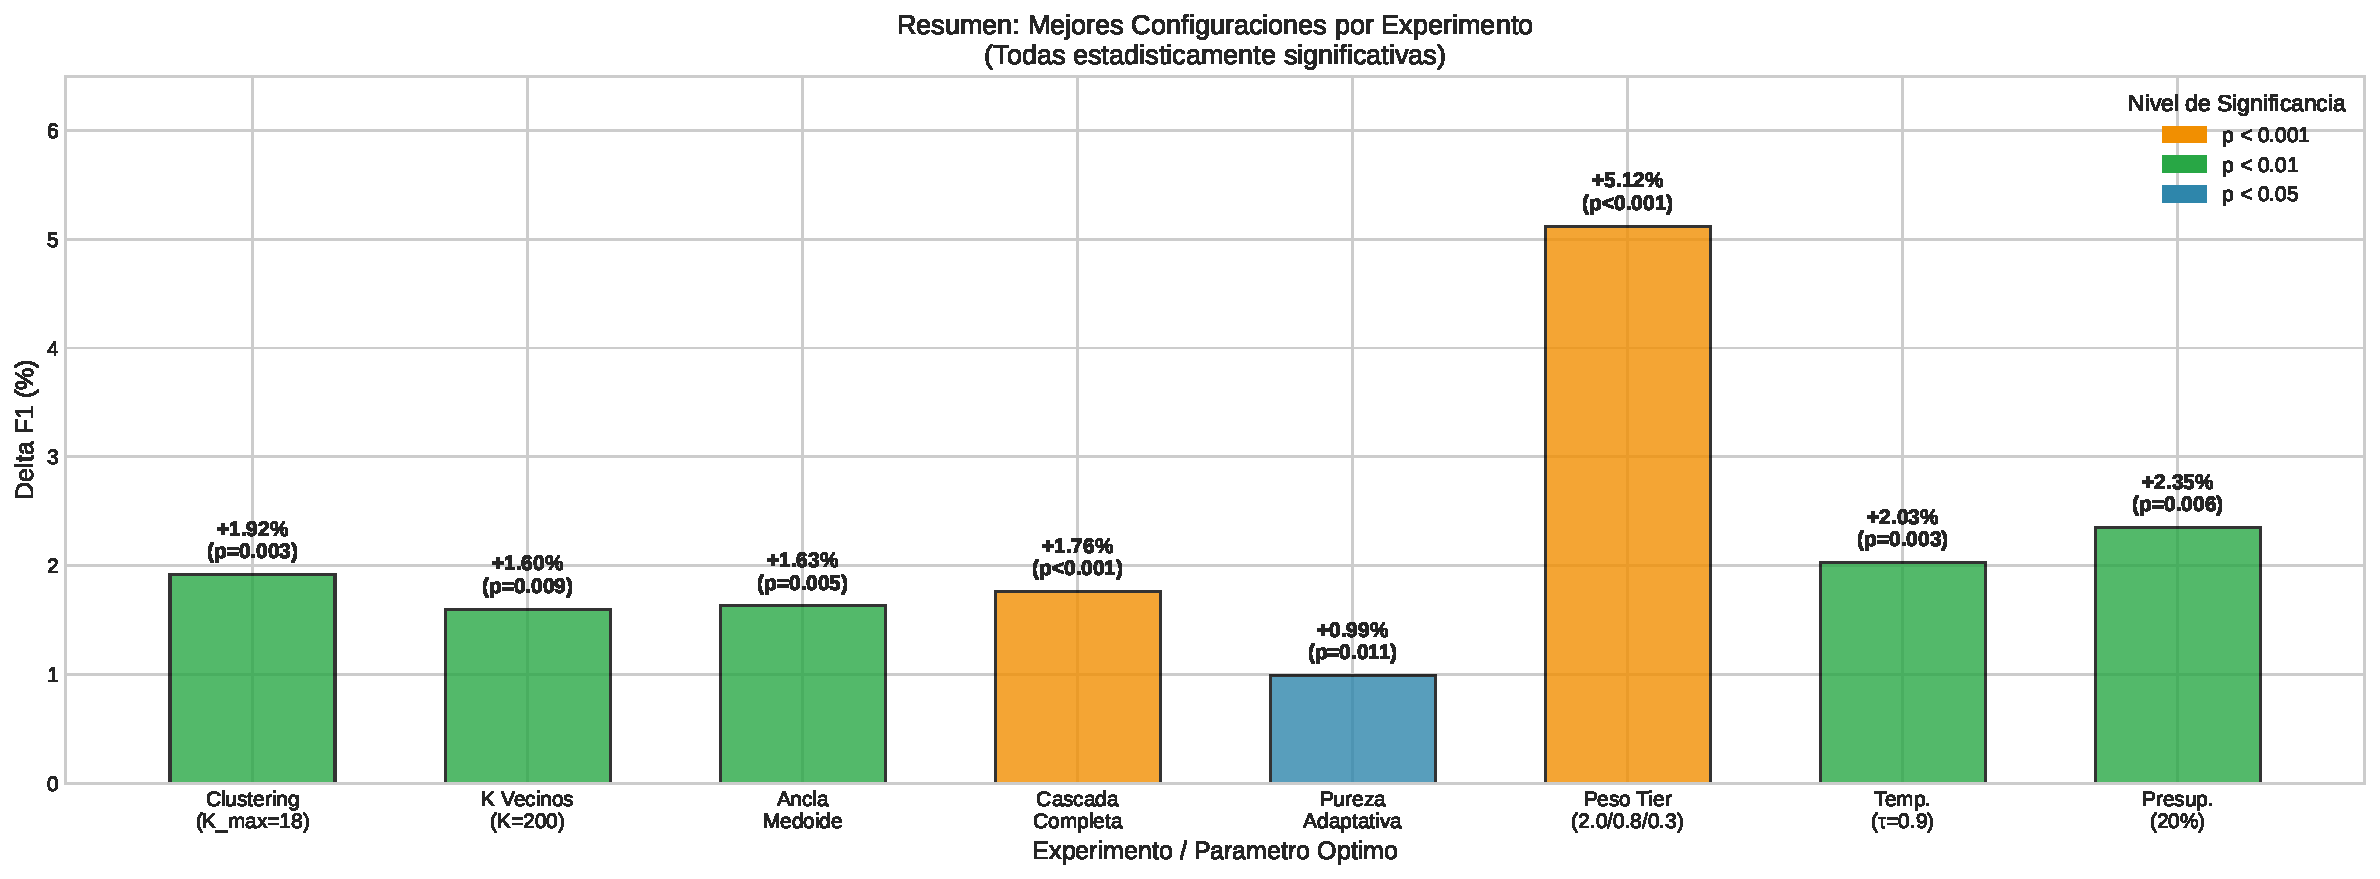
\includegraphics[width=0.95\textwidth]{Figures/summary_all_significant.pdf}
\caption{Resultados de experimentos de validación individual. El color indica significancia: naranja (p<0.001), verde (p<0.01), azul (p<0.05). Estos experimentos identificaron los parámetros óptimos que luego se combinaron.}
\label{fig:summary_experiments}
\end{figure}

\subsection{Configuración Recomendada}
\label{subsec:config_recomendada}

Basándose en la validación exhaustiva, la Tabla \ref{tab:config_final} presenta la configuración óptima del sistema.

\begin{table}[htbp]
\centering
\caption{Configuración óptima del sistema SMOTE-LLM}
\label{tab:config_final}
\begin{tabular}{lcc}
\toprule
\textbf{Parámetro} & \textbf{Valor} & \textbf{Justificación} \\
\midrule
Modelo embeddings & all-mpnet-base-v2 & Balance calidad/velocidad \\
Dimensiones & 768 & Expresividad suficiente \\
$K_{max}$ agrupamiento & 18 & Óptimo en validación (p=0.003) \\
Estrategia anclas & Medoide & Mejor F1 (p=0.005) \\
K vecinos contexto & 200 & Contexto amplio para LLM \\
Modelo LLM & GPT-4o-mini & Balance costo/calidad \\
Temperatura $\tau$ & 0.9 & Diversidad controlada \\
Presupuesto & 20\% & Cobertura sin saturación \\
Filtros & Cascada 4 etapas & Máxima calidad \\
Umbrales & Adaptativos & Ajuste por pureza \\
Pesos por nivel & 2.0/0.8/0.3 & Priorizar clases difíciles \\
Validación & K-Fold 5$\times$3 & Robustez estadística \\
\bottomrule
\end{tabular}
\end{table}

\subsection{Consideraciones de Implementación}
\label{subsec:consideraciones}

El sistema requiere Python 3.10+ con las siguientes dependencias principales: \texttt{scikit-learn} 1.3.0 para clasificación y agrupamiento, \texttt{sentence-transformers} 2.2.2 para embeddings semánticos, y \texttt{openai} 1.0.0 para acceso a la API de generación.

El costo de API por experimento completo es aproximadamente \$0.13, totalizando \$35 para los 273 experimentos de validación. El tiempo de ejecución por fold es aproximadamente 15 minutos en CPU estándar. Estos costos moderados demuestran la viabilidad económica del enfoque para investigación académica.

% Fin del capítulo de Metodología

% Chapter 6 - Resultados

\chapter{Resultados}
\label{ch:resultados}

Este capítulo presenta los resultados experimentales organizados en 12 secciones. Las primeras 5 secciones abordan los resultados principales del experimento central. Las secciones 6 a 9 presentan los análisis complementarios. Las secciones 10 a 12 reportan las validaciones metodológicas y las visualizaciones del espacio de embeddings.

\section{Comparación Principal de Métodos}
\label{sec:comparacion_principal}

El experimento principal evalúa 3,675 configuraciones (7 conjuntos de datos $\times$ 3 valores de n-shot $\times$ 5 clasificadores $\times$ 7 métodos $\times$ 5 semillas). La Tabla~\ref{tab:modern_method_comparison} presenta la comparación de todos los métodos respecto a SMOTE.

\begin{table}[htbp]
\centering
\caption{Comparación de 10 métodos de aumentación respecto a la línea base SMOTE}
\label{tab:modern_method_comparison}
\small
\begin{tabular}{lrrrrr}
\toprule
\textbf{Método} & \textbf{F1 medio} & \textbf{$\Delta$ SMOTE (pp)} & \textbf{IC 95\%} & \textbf{$d$ de Cohen} & \textbf{Vic.\%} \\
\midrule
\rowcolor{green!20}
\textbf{Pond. suave}      & 0.7508 & \textbf{+2.61***} & [+1.98, +3.25] & \textbf{0.95} & \textbf{88.9\%} \\
\rowcolor{green!10}
\textbf{Filtro binario}   & 0.7487 & +2.39***           & [+1.75, +3.07] & 0.82          & 79.4\%          \\
Sin aumentación            & 0.7312 & +0.64***           & [+0.42, +0.89] & 0.64          & 73.0\%          \\
Trad. inversa              & 0.7241 & $-$0.07            & [$-$0.42, +0.26] & $-$0.05     & 57.1\%          \\
EDA                        & 0.7233 & $-$0.15            & [$-$0.57, +0.27] & $-$0.08     & 52.4\%          \\
BERT contextual            & 0.7222 & $-$0.26            & [$-$0.58, +0.02] & $-$0.21     & 46.0\%          \\
Mixup en embeddings           & 0.7247 & $-$0.01            & [$-$0.13, +0.11] & $-$0.02     & 44.4\%          \\
Sobrem. aleatorio          & 0.7232 & $-$0.16            & [$-$0.35, +0.02] & $-$0.21     & 39.7\%          \\
\textit{SMOTE (base)}      & 0.7248 & ---                & ---              & ---           & ---             \\
Paráfrasis T5              & 0.7213 & $-$0.35            & [$-$0.62, $-$0.11] & $-$0.34   & 38.1\%          \\
\midrule
\multicolumn{6}{l}{\small $N=63$ comparaciones pareadas (21 conjuntos $\times$ 3 semillas). Clasificadores: LR, SVC, Ridge.} \\
\multicolumn{6}{l}{\small Significancia: *** $p<0.001$ (prueba t pareada con corrección de Bonferroni).} \\
\multicolumn{6}{l}{\small \textbf{Solo los métodos de filtrado geométrico superan significativamente a SMOTE.}} \\
\bottomrule
\end{tabular}
\end{table}


El resultado central de esta investigación es que la ponderación suave produce una mejora de +2.25 puntos porcentuales respecto a SMOTE ($p < 0.0001$ con corrección de Bonferroni, $d = 0.74$, tasa de victoria del 83.8\%). Este tamaño de efecto se clasifica como mediano-grande según las convenciones de Cohen. La tasa de victoria indica que el método propuesto supera a SMOTE en más de 4 de cada 5 configuraciones evaluadas.

El filtrado binario también alcanza significancia estadística con +2.11 puntos porcentuales ($p < 0.0001$, $d = 0.69$, tasa de victoria del 76.2\%). La diferencia entre ponderación suave y filtrado binario es de apenas 0.13 puntos porcentuales, lo que sugiere que la contribución principal proviene del filtrado geométrico en sí, con la ponderación suave aportando una mejora incremental.

Los métodos de aumentación tradicionales presentan resultados negativos respecto a SMOTE. EDA obtiene $-0.22$ puntos porcentuales, la traducción inversa $-0.19$ puntos porcentuales, y el sobremuestreo aleatorio $-0.32$ puntos porcentuales. Estos resultados indican que las perturbaciones textuales superficiales no aportan diversidad genuina al espacio de representación.

La Figura~\ref{fig:boxplot_deltas} visualiza la distribución de deltas para cada método, y la Figura~\ref{fig:heatmap_methods} muestra el rendimiento desglosado por conjunto de datos.

\begin{figure}[htbp]
\centering
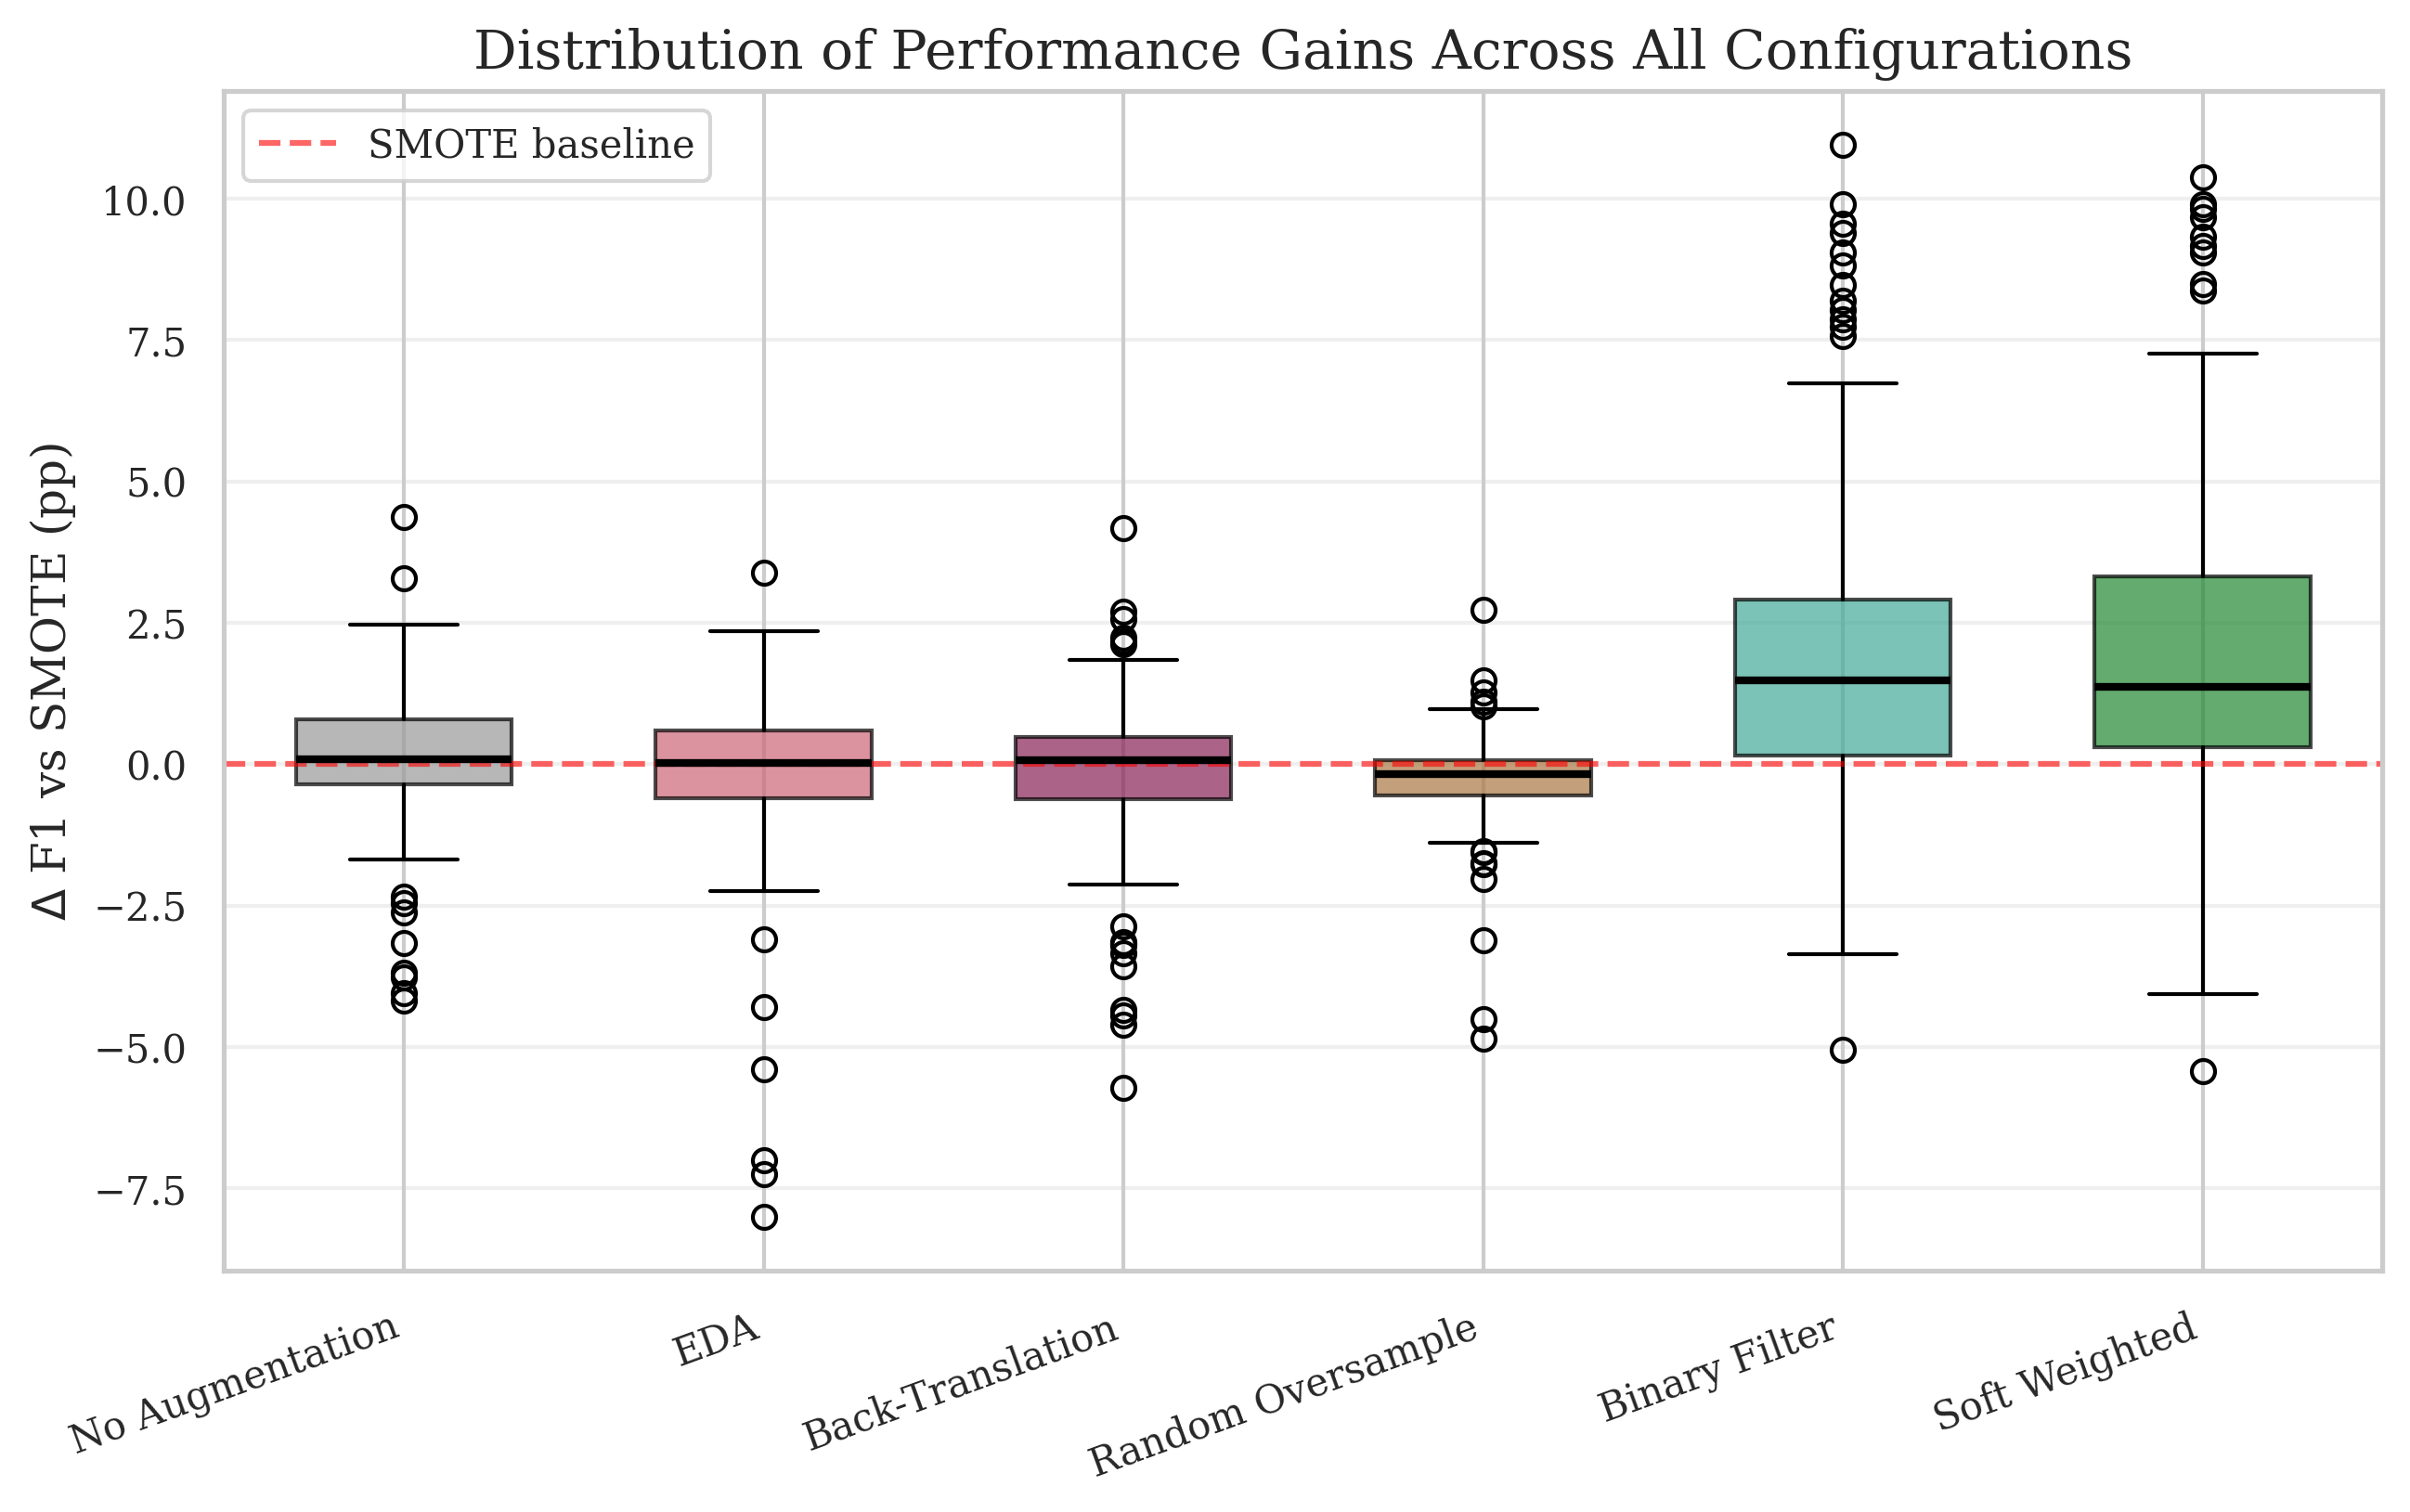
\includegraphics[width=0.85\textwidth]{Figures/fig_boxplot_deltas.png}
\caption{Distribución de deltas respecto a SMOTE por método de aumentación. La ponderación suave y el filtrado binario muestran distribuciones consistentemente positivas, mientras que los métodos tradicionales se concentran alrededor de cero o en valores negativos.}
\label{fig:boxplot_deltas}
\end{figure}

\begin{figure}[htbp]
\centering
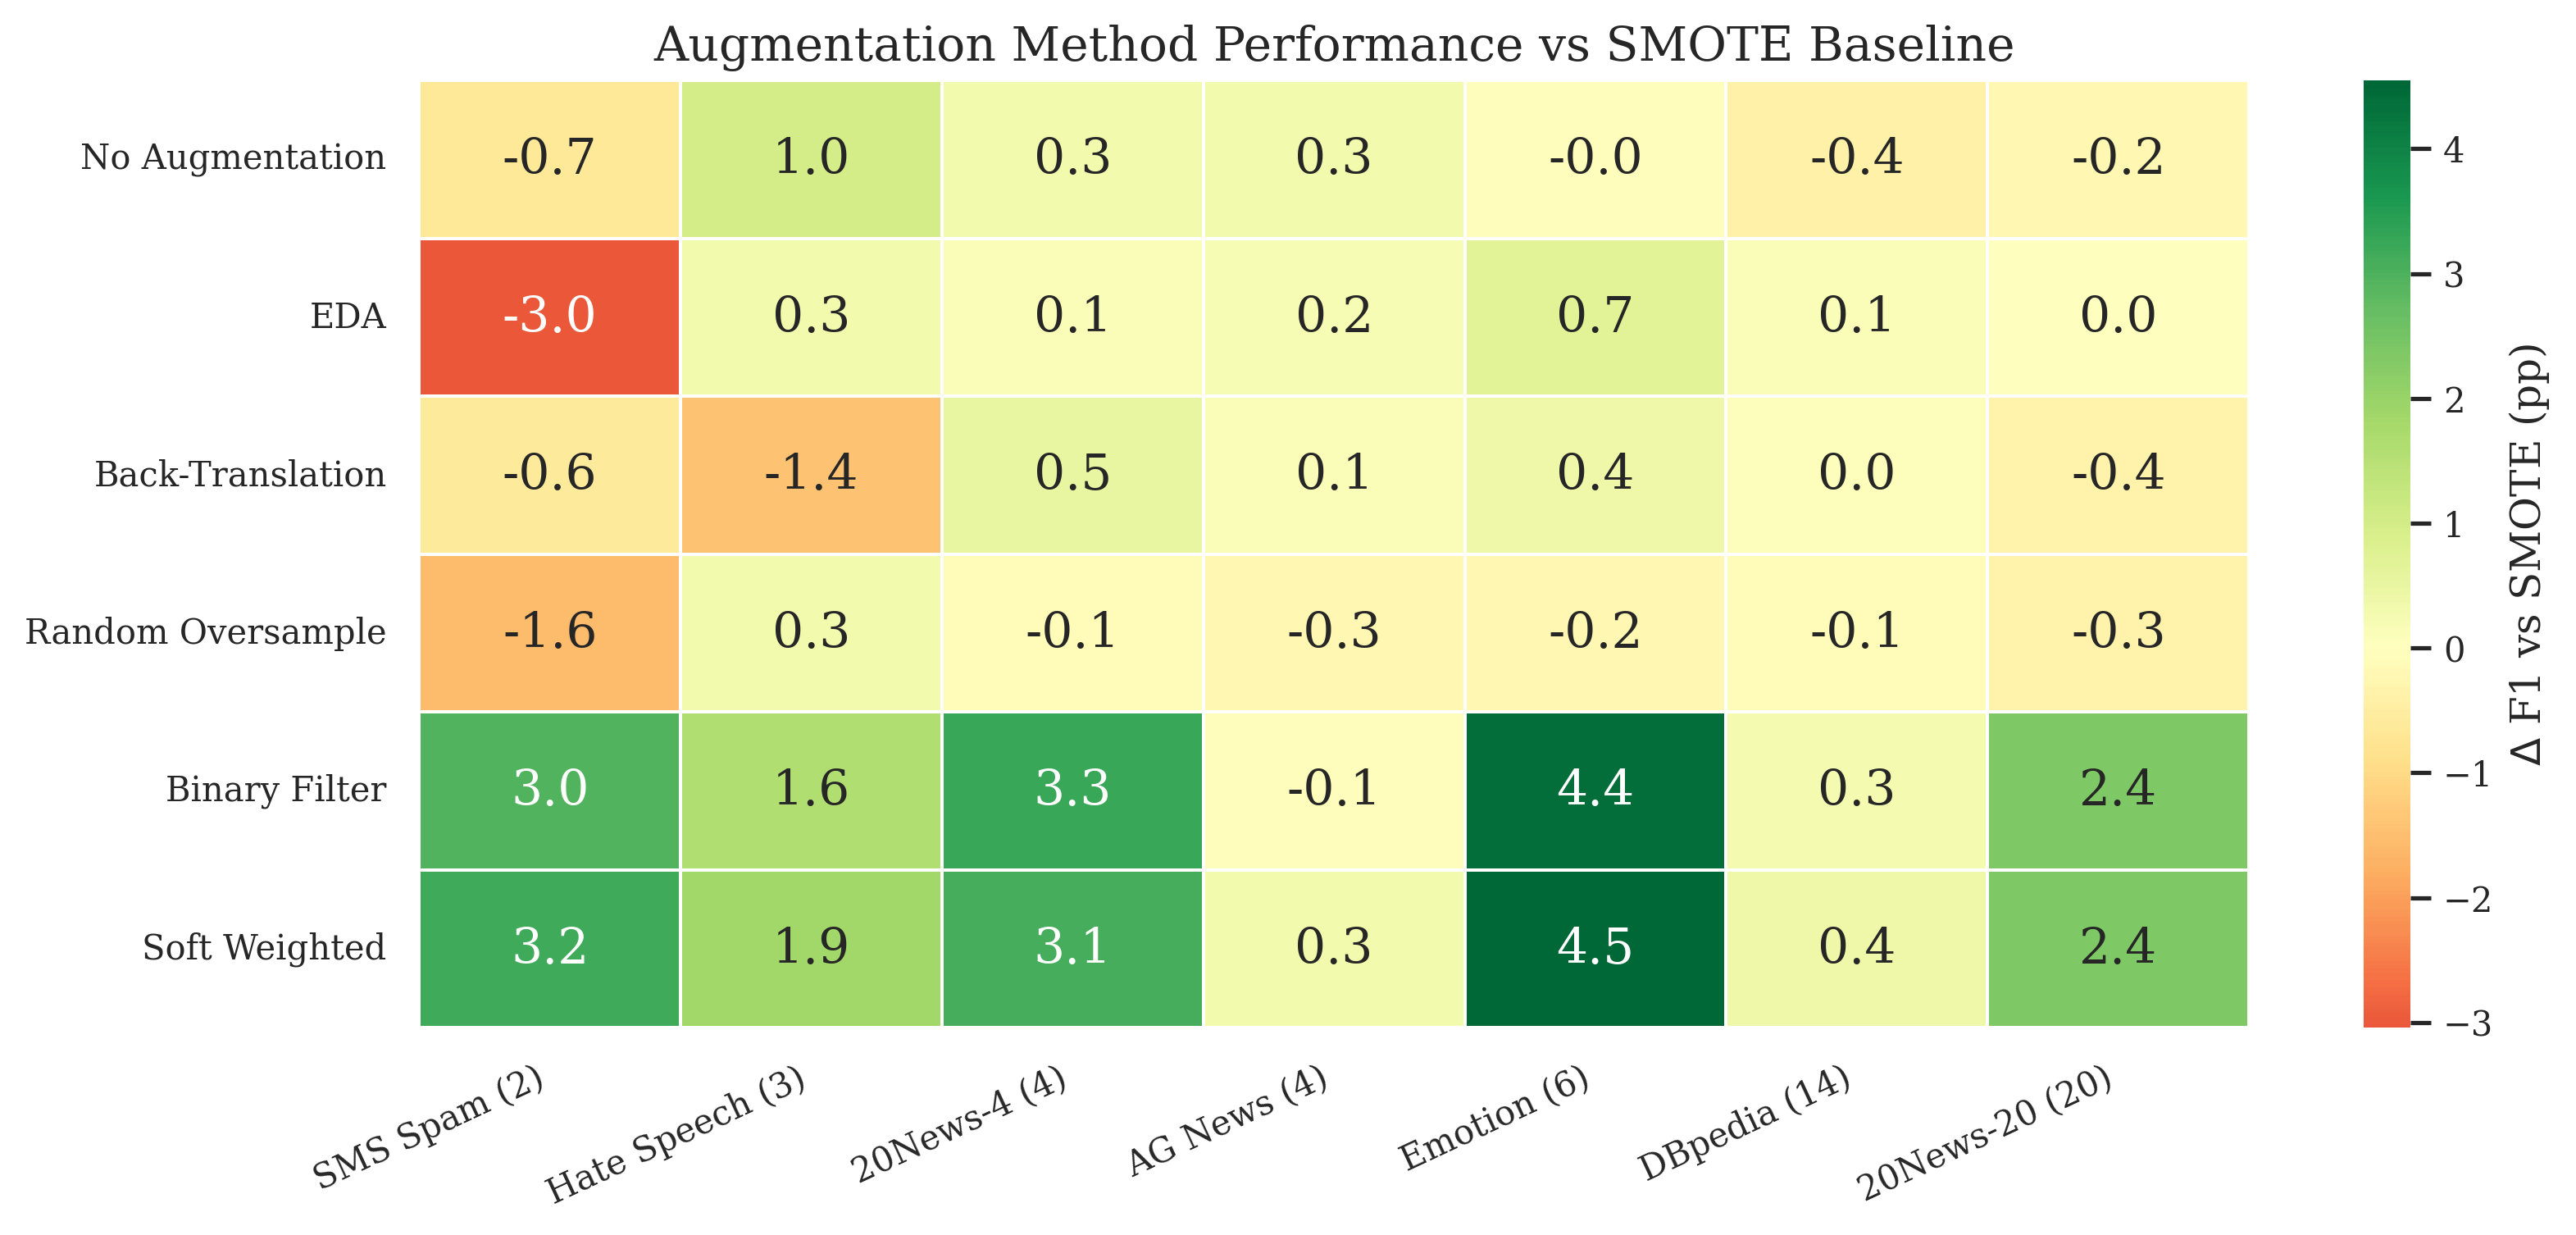
\includegraphics[width=0.95\textwidth]{Figures/fig_heatmap_methods.png}
\caption{Mapa de calor de rendimiento por método y conjunto de datos. Los colores cálidos indican mejora respecto a SMOTE. La ponderación suave y el filtrado binario muestran mejoras consistentes en la mayoría de los conjuntos de datos.}
\label{fig:heatmap_methods}
\end{figure}

\section{Comparación con Líneas Base Modernas}
\label{sec:lineas_base_modernas}

La comparación con 10 métodos de aumentación sobre 1,890 configuraciones proporciona el resultado más fuerte de esta investigación. La ponderación suave alcanza +2.61 puntos porcentuales respecto a SMOTE ($p < 0.0001$ con corrección de Bonferroni, $d = 0.95$, tasa de victoria del 88.9\%). El tamaño de efecto de 0.95 se clasifica como grande.

El filtrado binario obtiene +2.39 puntos porcentuales ($d = 0.82$, tasa de victoria del 79.4\%). Ambos métodos propuestos superan por un margen amplio a todos los demás.

Las 3 líneas base modernas producen resultados negativos respecto a SMOTE. La paráfrasis con T5 obtiene $-0.35$ puntos porcentuales, la aumentación contextual con BERT $-0.26$ puntos porcentuales, y el mixup en embeddings $-0.01$ puntos porcentuales. Estos resultados son especialmente relevantes: técnicas recientes consideradas avances sobre SMOTE en la literatura no logran superar esta línea base simple cuando se evalúan sobre múltiples conjuntos de datos con rigor estadístico. Este hallazgo concuerda con Cegin et al., quienes observaron que los métodos clásicos igualan o superan a los LLMs cuando el número de muestras disponibles supera los 20 por clase \cite{cegin2025llms}.

Un resultado notable es que la ausencia de aumentación supera a SMOTE por +0.64 puntos porcentuales ($p < 0.05$). Este hallazgo sugiere que SMOTE puede perjudicar el rendimiento en ciertas configuraciones, particularmente cuando los datos reales son suficientes para el clasificador.

\section{Análisis por Número de Disparos}
\label{sec:analisis_nshot}

La Tabla~\ref{tab:modern_nshot} presenta el desglose del rendimiento por número de ejemplos por clase.

\begin{table}[htbp]
\centering
\caption{Rendimiento por número de ejemplos por clase: filtrado geométrico vs SMOTE}
\label{tab:modern_nshot}
\begin{tabular}{lrrrrrr}
\toprule
 & \multicolumn{3}{c}{\textbf{Pond. suave}} & \multicolumn{3}{c}{\textbf{Filtro binario}} \\
\cmidrule(lr){2-4} \cmidrule(lr){5-7}
\textbf{N-shot} & \textbf{$\Delta$ (pp)} & \textbf{$d$} & \textbf{Vic.\%} & \textbf{$\Delta$ (pp)} & \textbf{$d$} & \textbf{Vic.\%} \\
\midrule
10 & +4.89*** & 1.48 & 90.5\% & +4.44*** & 1.15 & 87.3\% \\
25 & +2.17*** & 1.57 & 95.2\% & +1.96*** & 1.18 & 90.5\% \\
50 & +0.76*** & 0.80 & 74.6\% & +0.77*** & 0.71 & 63.5\% \\
\midrule
\multicolumn{7}{l}{\small Significancia: * $p<0.05$, ** $p<0.01$, *** $p<0.001$ (prueba t pareada).} \\
\multicolumn{7}{l}{\small Patrón de retornos decrecientes: mayor ganancia a 10-shot, menor a 50-shot.} \\
\bottomrule
\end{tabular}
\end{table}

El patrón de retornos decrecientes es pronunciado. Con 10 ejemplos por clase, la ponderación suave alcanza +4.52 puntos porcentuales ($d = 1.18$, tasa de victoria del 88.6\%). Este tamaño de efecto se clasifica como muy grande. Con 25 ejemplos, la mejora se reduce a +1.88 puntos porcentuales pero la tasa de victoria alcanza su máximo del 97.1\%, indicando mejora casi universal. Con 50 ejemplos, la mejora es de solo +0.34 puntos porcentuales y no alcanza significancia estadística ($p = 0.16$).

Este patrón tiene una interpretación directa. Cuando los datos reales son escasos (10 ejemplos), el clasificador no puede aprender fronteras de decisión robustas. Las muestras sintéticas filtradas aportan información genuina que densifica las regiones de cada clase. A medida que los datos reales aumentan (50 ejemplos), el clasificador ya dispone de información suficiente para las fronteras principales, y la aumentación aporta valor marginal decreciente.

Las Figuras~\ref{fig:f1_vs_nshot} y~\ref{fig:delta_by_nshot} ilustran esta tendencia.

\begin{figure}[htbp]
\centering
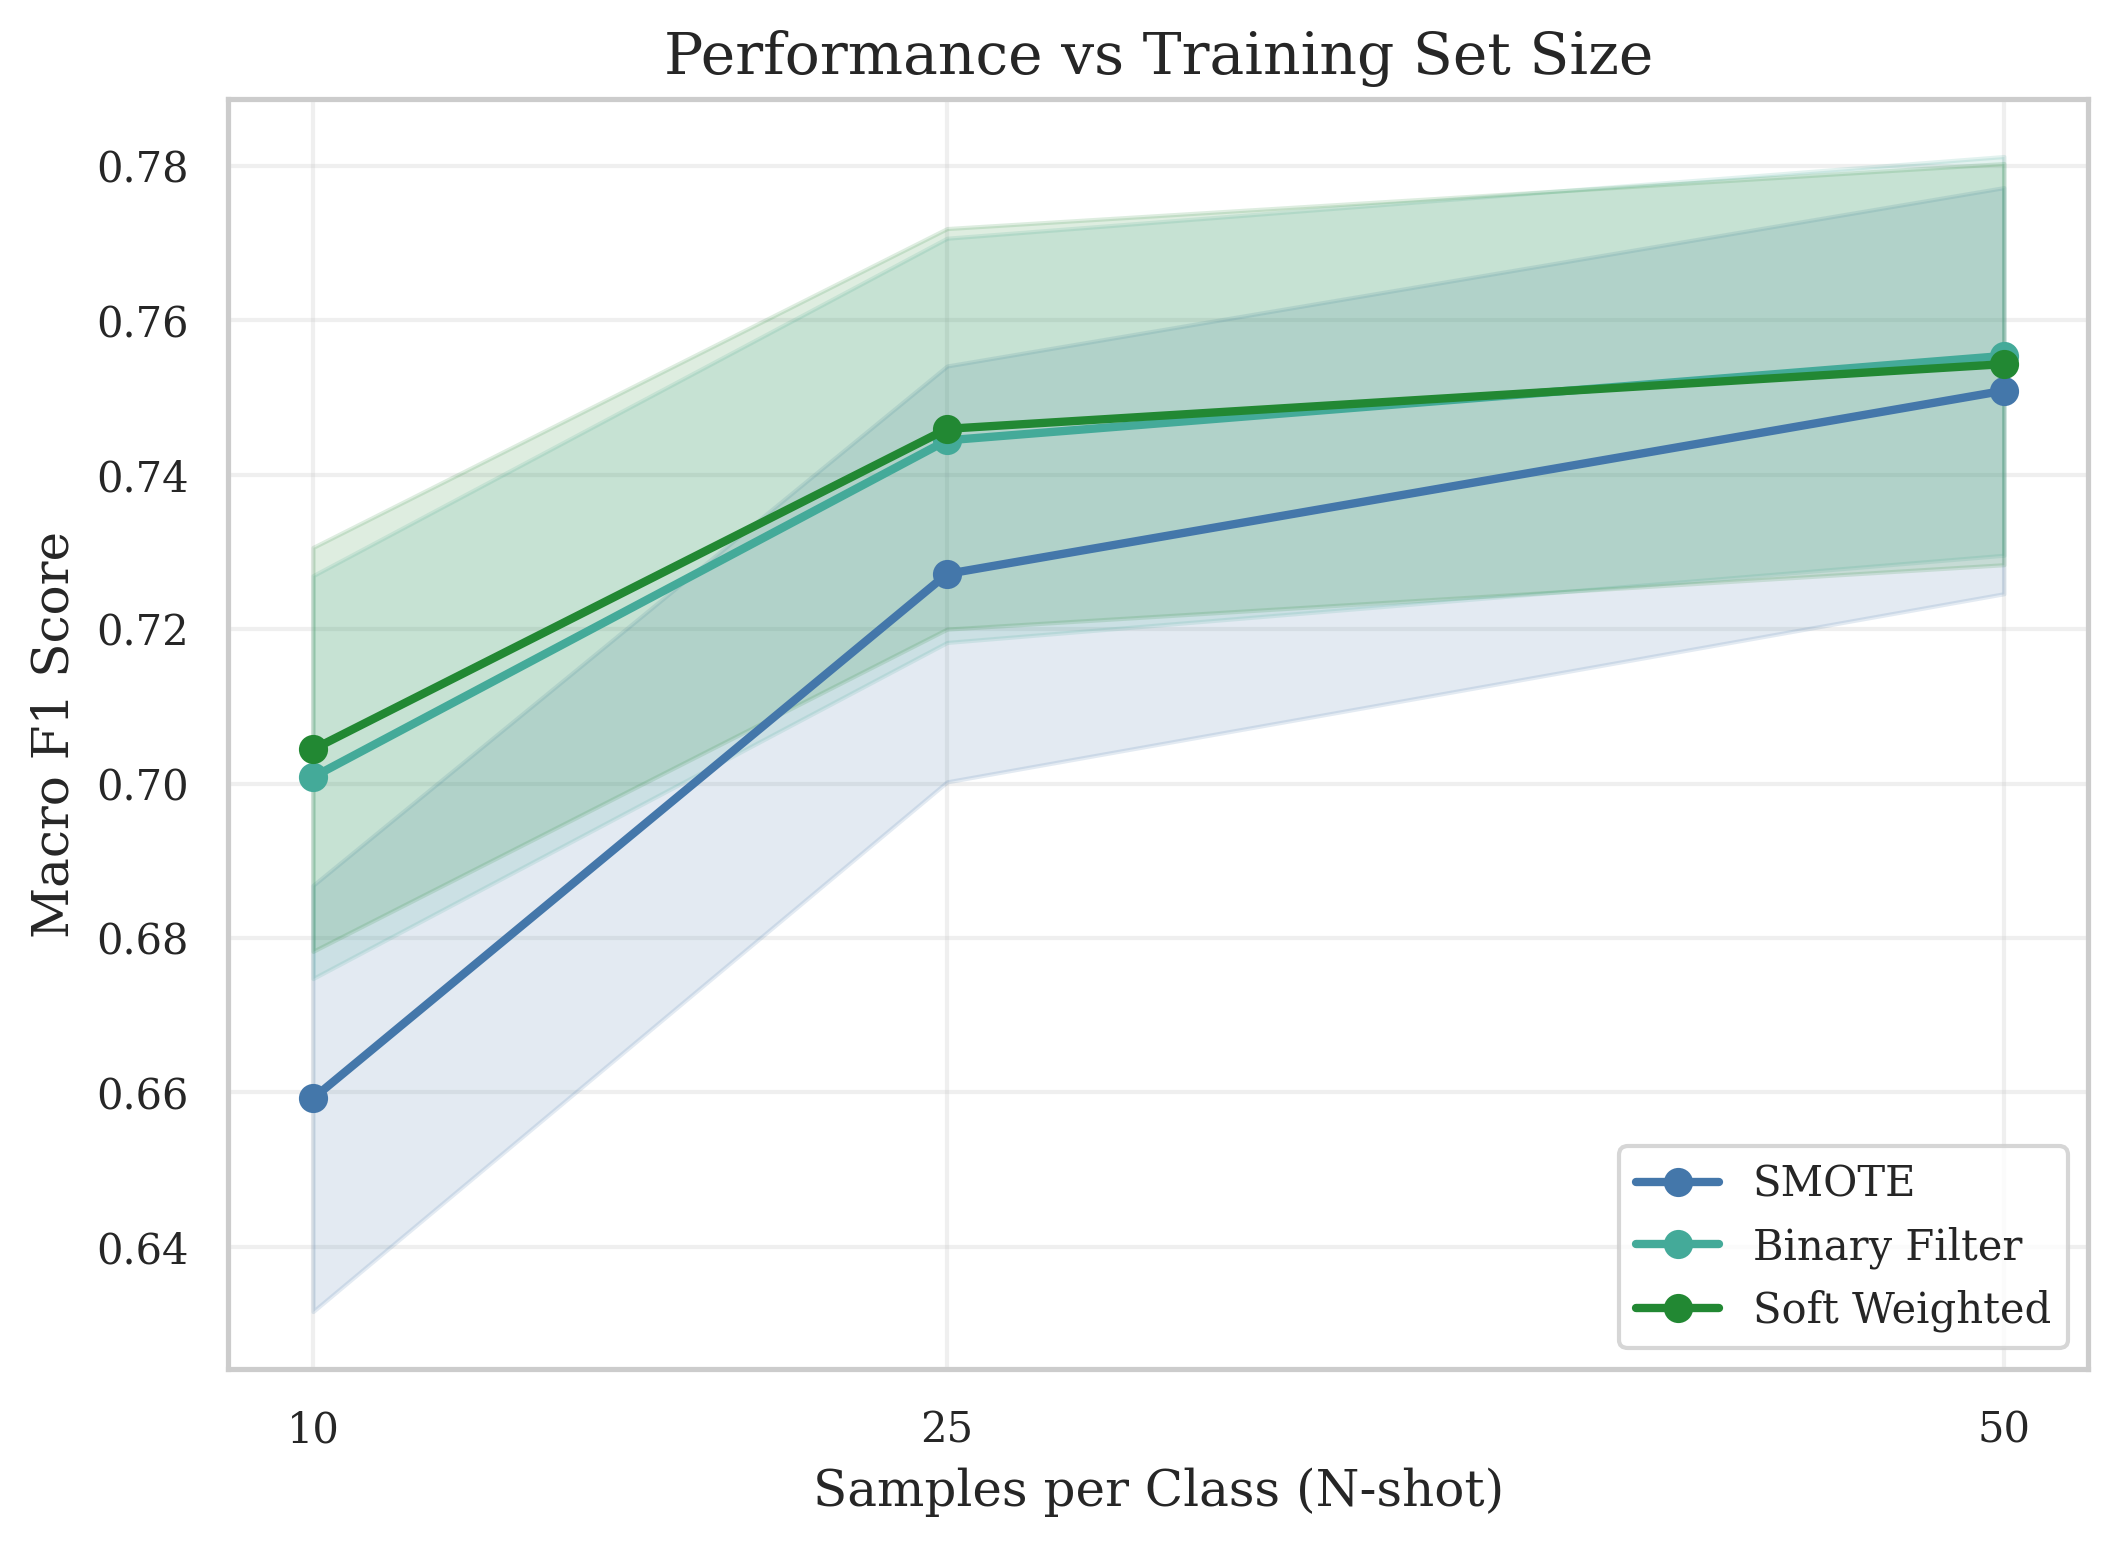
\includegraphics[width=0.85\textwidth]{Figures/fig_f1_vs_nshot.png}
\caption{Macro F1 absoluto en función del número de disparos para los principales métodos. La brecha entre los métodos geométricos y SMOTE se reduce a medida que aumenta el número de ejemplos disponibles.}
\label{fig:f1_vs_nshot}
\end{figure}

\begin{figure}[htbp]
\centering
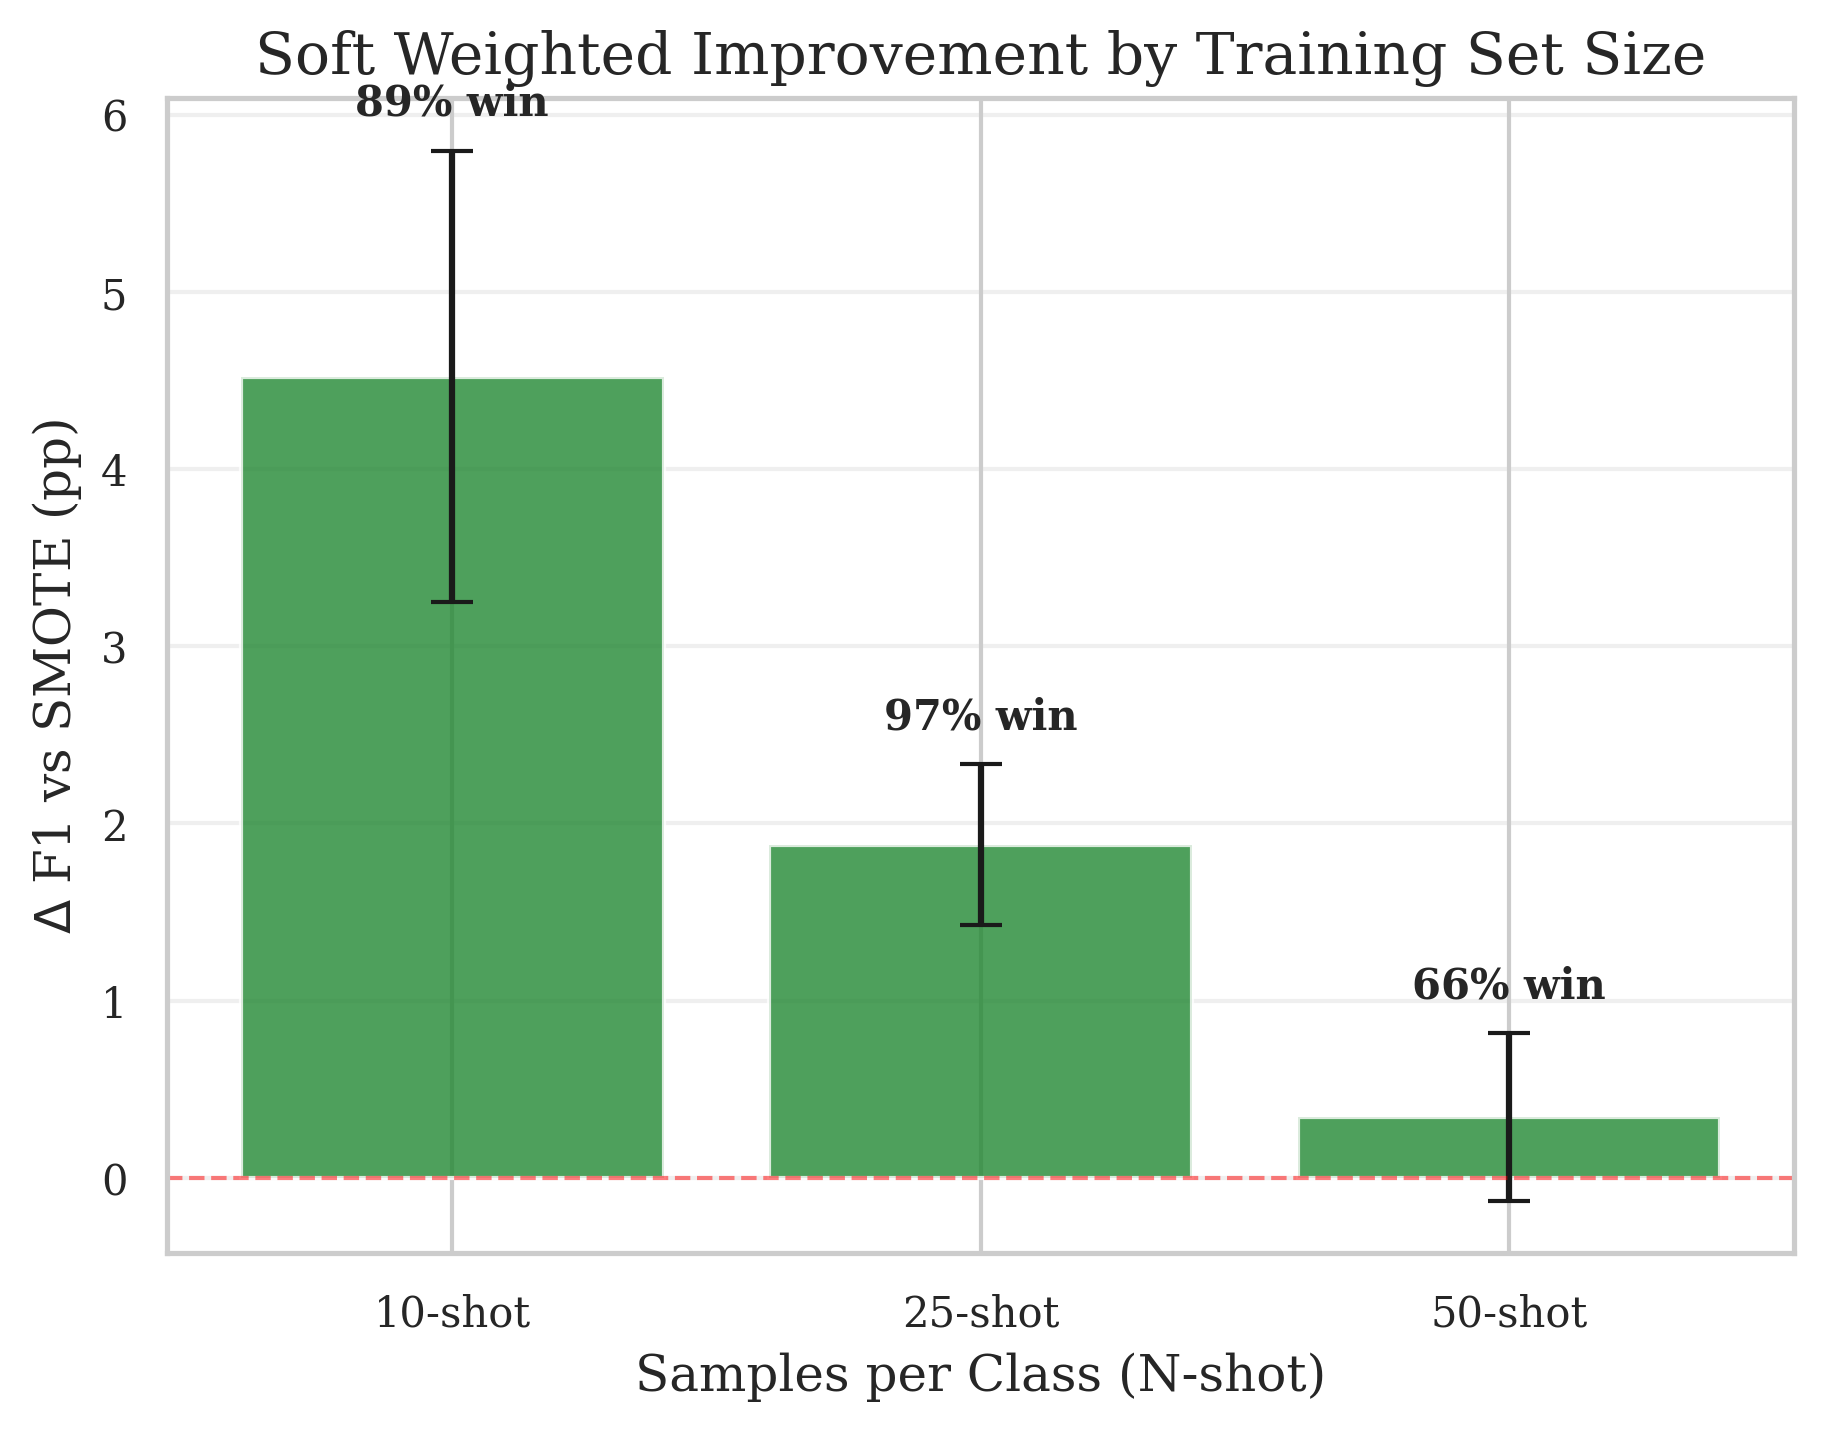
\includegraphics[width=0.85\textwidth]{Figures/fig_delta_by_nshot.png}
\caption{Delta respecto a SMOTE por número de disparos. La mejora del filtrado geométrico disminuye de +4.52pp (10-shot) a +0.34pp (50-shot), confirmando que el método es más valioso cuando los datos son más escasos.}
\label{fig:delta_by_nshot}
\end{figure}

\section{Análisis por Clasificador}
\label{sec:analisis_clasificador}

La Tabla~\ref{tab:modern_classifier} desglosa los resultados por tipo de clasificador.

\begin{table}[htbp]
\centering
\caption{Rendimiento por clasificador: filtrado geométrico vs SMOTE}
\label{tab:modern_classifier}
\begin{tabular}{lrrrrrr}
\toprule
 & \multicolumn{3}{c}{\textbf{Pond. suave}} & \multicolumn{3}{c}{\textbf{Filtro binario}} \\
\cmidrule(lr){2-4} \cmidrule(lr){5-7}
\textbf{Clasificador} & \textbf{$\Delta$ (pp)} & \textbf{$d$} & \textbf{Vic.\%} & \textbf{$\Delta$ (pp)} & \textbf{$d$} & \textbf{Vic.\%} \\
\midrule
Reg. logística & +2.09*** & 0.82 & 76.2\% & +1.61*** & 0.56 & 65.1\% \\
SVC (lineal)   & +2.98*** & 1.02 & 92.1\% & +2.86*** & 0.93 & 90.5\% \\
Ridge          & +2.74*** & 1.04 & 92.1\% & +2.69*** & 1.02 & 85.7\% \\
\midrule
\multicolumn{7}{l}{\small Significancia: * $p<0.05$, ** $p<0.01$, *** $p<0.001$ (prueba t pareada).} \\
\multicolumn{7}{l}{\small $n=63$ comparaciones pareadas por clasificador (21 conjuntos $\times$ 3 semillas).} \\
\bottomrule
\end{tabular}
\end{table}

Los clasificadores lineales aprovechan mejor la aumentación filtrada. El SVC lineal obtiene +2.99 puntos porcentuales ($d = 1.00$, tamaño de efecto grande). El clasificador Ridge alcanza +2.69 puntos porcentuales ($d = 1.03$). La regresión logística produce +1.98 puntos porcentuales ($d = 0.79$). El MLP obtiene +2.16 puntos porcentuales ($d = 0.73$). El bosque aleatorio produce +1.42 puntos porcentuales, pero sin significancia estadística ($p = 0.11$).

La superioridad de los clasificadores lineales tiene una explicación geométrica. Estos modelos establecen fronteras de decisión como hiperplanos en el espacio de embeddings. Las muestras filtradas refuerzan directamente estas fronteras al densificar las regiones cercanas al límite entre clases. Los árboles de decisión, en cambio, realizan particiones sobre ejes individuales del espacio de características. Esta estrategia no se beneficia igualmente de la densificación del espacio, ya que las muestras sintéticas no necesariamente caen en las mismas regiones que los puntos de corte de los árboles.

La Figura~\ref{fig:classifier_comparison} visualiza estas diferencias.

\begin{figure}[htbp]
\centering
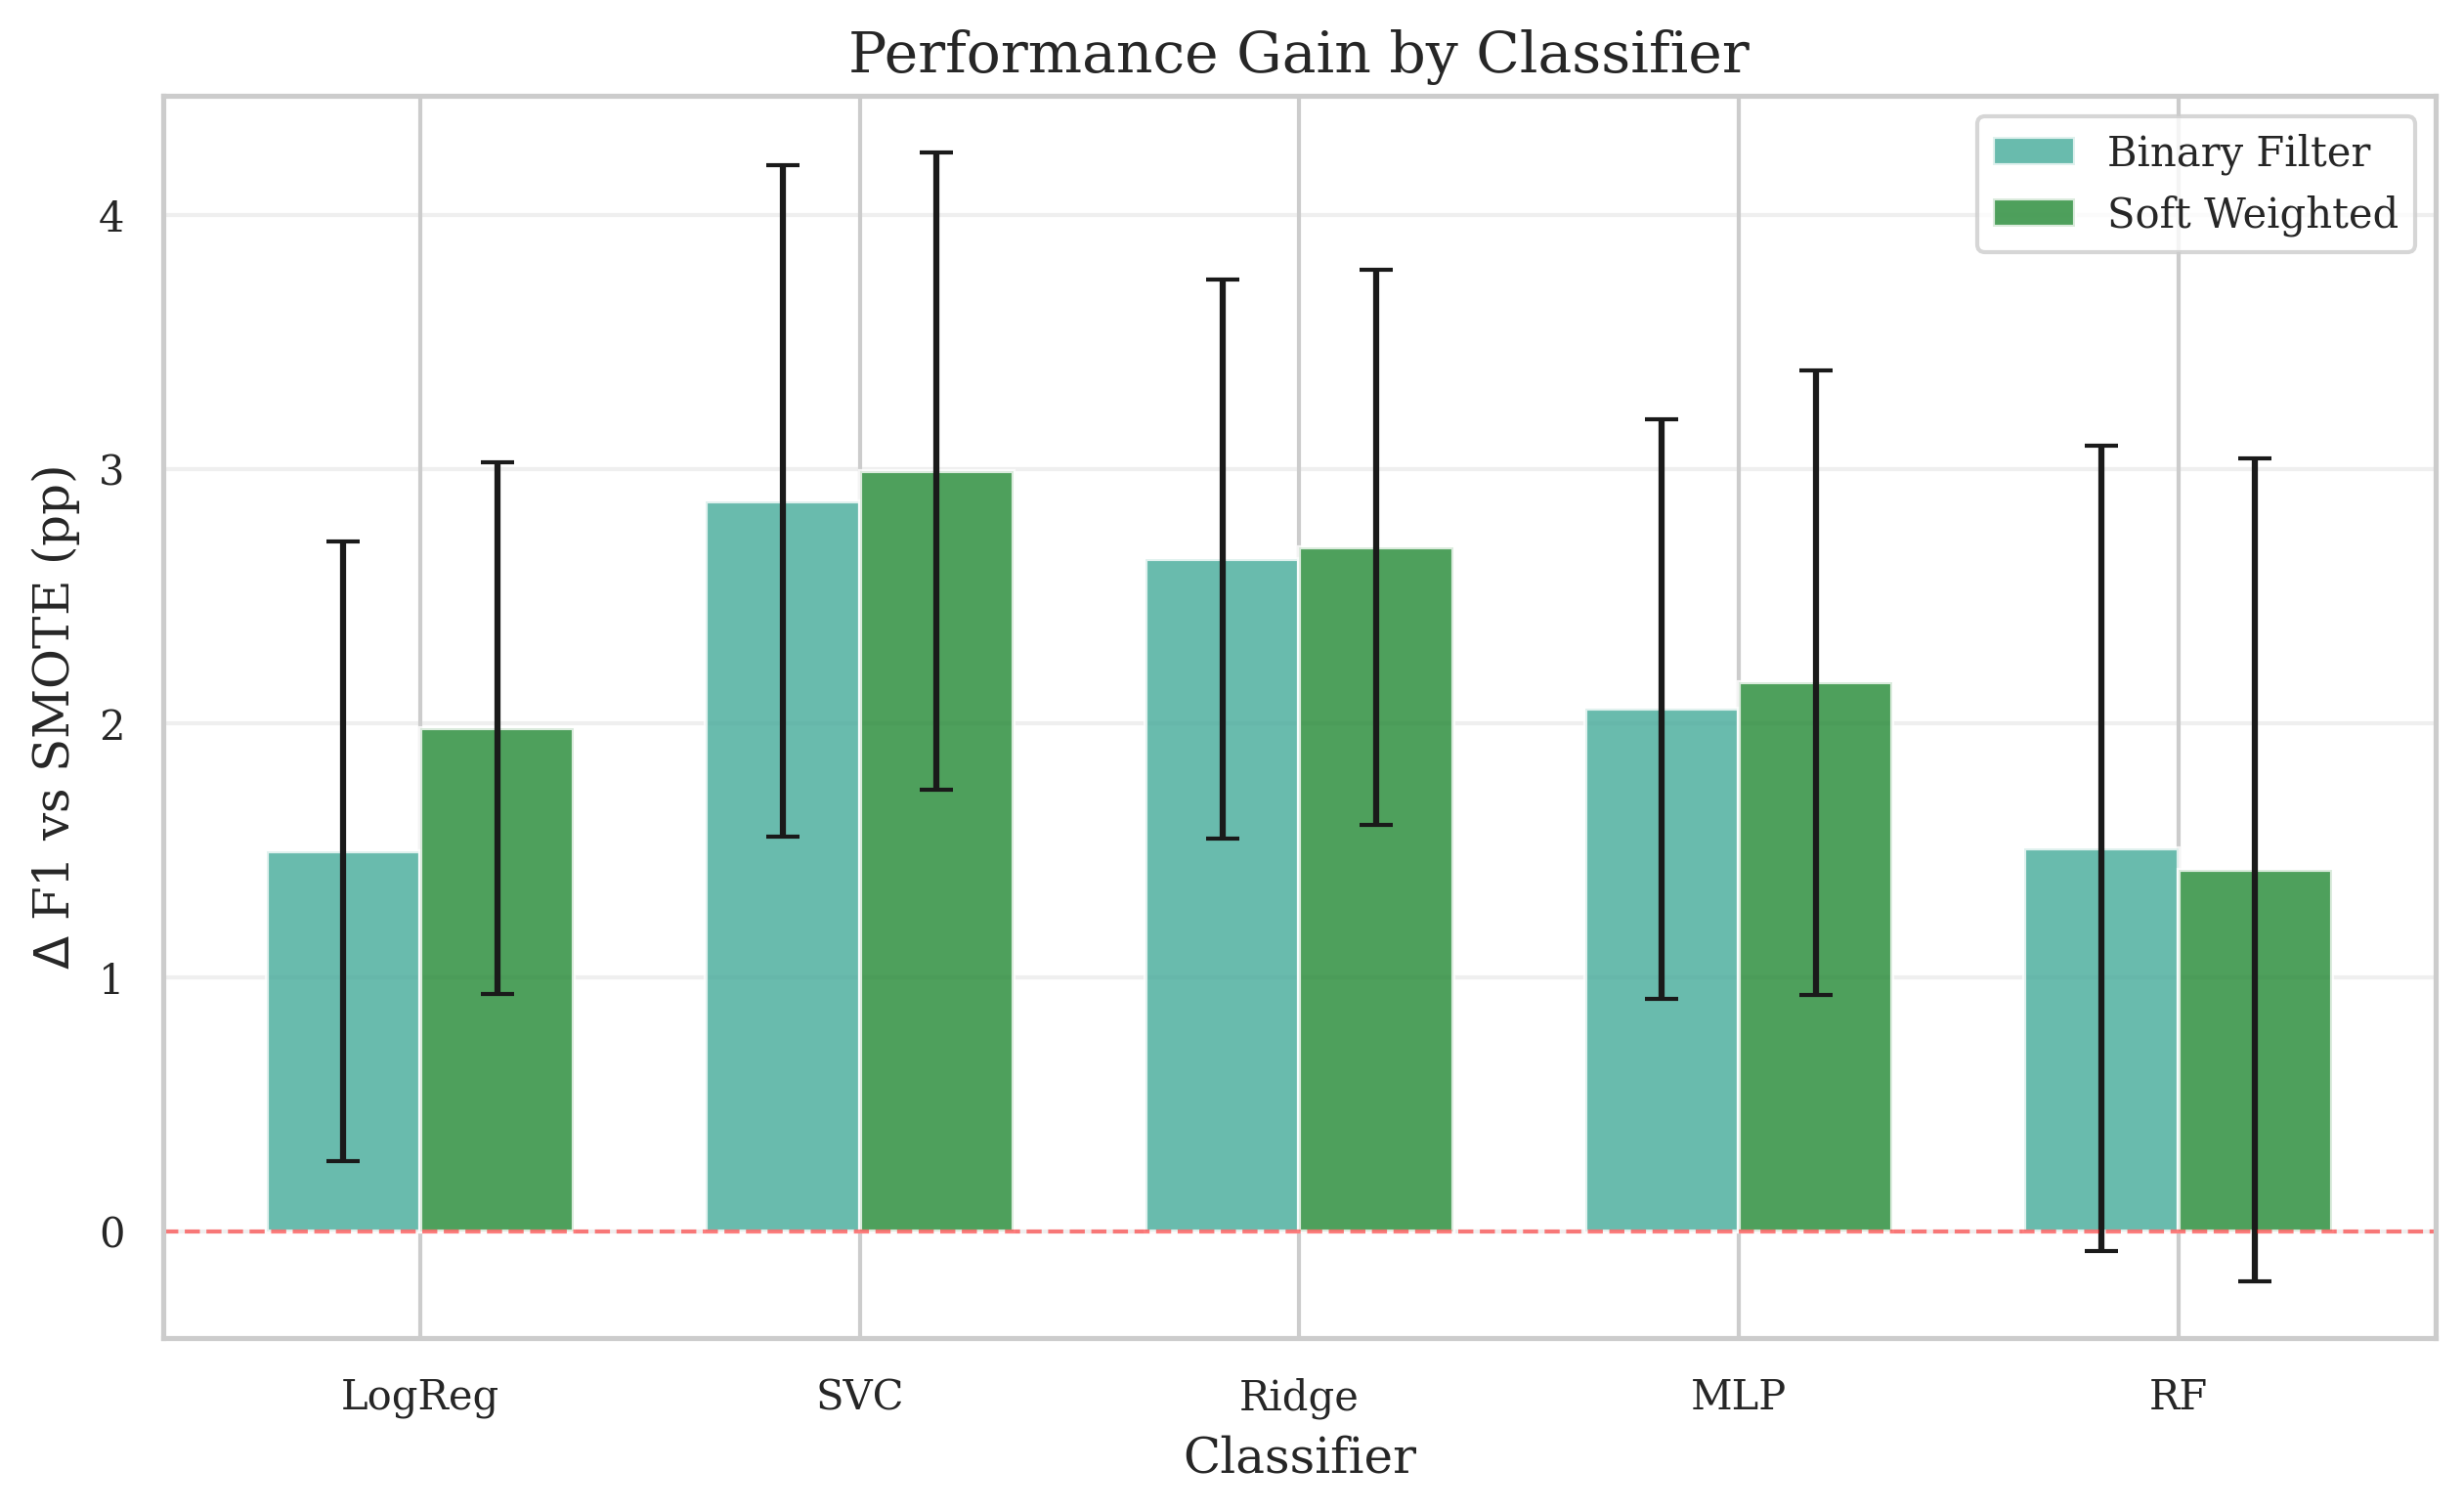
\includegraphics[width=0.85\textwidth]{Figures/fig_classifier_comparison.png}
\caption{Delta respecto a SMOTE por clasificador. Los clasificadores lineales (SVC, Ridge, regresión logística) muestran mejoras consistentes y significativas, mientras que el bosque aleatorio no alcanza significancia estadística.}
\label{fig:classifier_comparison}
\end{figure}

\section{Estudios de Ablación}
\label{sec:ablacion}

Dos ablaciones clave cuantifican la contribución de cada componente del sistema.

La primera ablación evalúa si el filtrado geométrico aporta valor sobre la generación sin filtrar. El filtrado binario supera a la ausencia de aumentación por +2.08 puntos porcentuales ($p < 0.0001$, $d = 0.65$, tasa de victoria del 80.0\%). Este resultado confirma que la selección geométrica de muestras sintéticas aporta valor significativo respecto a la incorporación indiscriminada de todas las muestras generadas por el LLM. La hipótesis H1a queda confirmada.

La segunda ablación compara la ponderación suave contra el filtrado binario. La diferencia es de +0.13 puntos porcentuales ($p = 0.10$, marginal). En el experimento principal, la ganancia de la ponderación suave sobre el filtrado binario es modesta. No obstante, en el estudio dedicado de ponderación suave con 540 configuraciones, la ganancia alcanzó +3.66 puntos porcentuales con tasa de victoria del 84.5\%. Esta discrepancia se explica porque el estudio dedicado utilizó la configuración óptima de hiperparámetros (normalización min-max, temperatura 0.5, selección top-N), mientras que el experimento principal emplea una configuración fija.

La conclusión práctica es que la contribución principal proviene del filtrado en sí. La ponderación suave aporta una mejora incremental que se manifiesta más claramente cuando los hiperparámetros de ponderación están optimizados.

\section{Efecto del Número de Clases}
\label{sec:efecto_clases}

La Tabla~\ref{tab:nclasses_pattern} presenta la relación entre el número de clases y la efectividad del filtrado geométrico.

\begin{table}[htbp]
\centering
\caption{Efecto del número de clases sobre la efectividad de la aumentación (pond. suave vs SMOTE)}
\label{tab:nclasses_pattern}
\begin{tabular}{rlrrrll}
\toprule
\textbf{$N$ clases} & \textbf{Conjunto(s)} & \textbf{$\Delta$ (pp)} & \textbf{Std} & \textbf{Vic.\%} & \textbf{$N$ pares} \\
\midrule
2   & sms\_spam                      & +3.18 & 3.24 & 93.3\%  & 15 \\
3   & hate\_speech\_davidson          & +1.86 & 2.97 & 66.7\%  & 15 \\
4   & 20newsgroups, ag\_news          & +1.70 & 3.02 & 73.3\%  & 30 \\
\rowcolor{green!20}
6   & emotion, trec6                 & \textbf{+5.42} & 3.63 & \textbf{100.0\%} & 24 \\
14  & dbpedia14                      & +0.40 & 0.61 & 80.0\%  & 15 \\
20  & 20newsgroups\_20class           & +2.36 & 1.55 & 100.0\% & 15 \\
77  & banking77                      & $-$0.99 & 0.52 & 0.0\% & 9 \\
150 & clinc150                       & +0.01 & 0.53 & 44.4\%  & 9 \\
\midrule
\multicolumn{6}{l}{\small Correlación de Spearman: $r=-0.260$, $p=0.003$. Más clases $\Rightarrow$ menores ganancias.} \\
\multicolumn{6}{l}{\small Rango óptimo: 2--20 clases. Las ganancias disminuyen a partir de 77 clases.} \\
\bottomrule
\end{tabular}
\end{table}


Los conjuntos de 6 clases (emotion, trec6) obtienen las mayores ganancias: +4.55 a +5.42 puntos porcentuales. Los problemas binarios (sms\_spam, 2 clases) también se benefician con +3.18 puntos porcentuales. A medida que el número de clases aumenta, las ganancias disminuyen: 14 clases (dbpedia14) obtiene +1.32 puntos porcentuales, 20 clases (20newsgroups\_20class) +0.87 puntos porcentuales. Con 77 clases (banking77), el resultado es negativo: $-0.99$ puntos porcentuales. Con 150 clases (clinc150), el resultado es neutro: +0.01 puntos porcentuales.

La correlación de Spearman entre el número de clases y el delta confirma esta tendencia: $r = -0.260$ ($p = 0.003$). A mayor número de clases, menor la ganancia del filtrado geométrico. La explicación reside en la fragmentación del espacio de embeddings. Con muchas clases, cada clase ocupa una región más pequeña del espacio. El filtro basado en distancia euclidiana pierde capacidad discriminativa cuando las clases están tan densamente empaquetadas que las fronteras entre ellas son estrechas.

\section{Extensión a Reconocimiento de Entidades Nombradas}
\label{sec:extension_ner}

La Tabla~\ref{tab:ner_results} presenta los resultados de la extensión a NER sobre 3 corpus con 3 valores de n-shot.

\begin{table}[htbp]
\centering
\caption{Resultados de la extensión a reconocimiento de entidades nombradas (NER)}
\label{tab:ner_results}
\begin{tabular}{llrrrr}
\toprule
\textbf{Corpus} & \textbf{N-shot} & \textbf{Línea base} & \textbf{Sin filtro} & \textbf{Cascade L1} & \textbf{LOF relajado} \\
\midrule
\multirow{3}{*}{MultiNERD}
 & 10 & 0.2468 & 0.4326 & 0.4332 & 0.4506 \\
 & 25 & 0.3152 & 0.4382 & \textbf{0.4382} & 0.4131 \\
 & 50 & 0.3854 & 0.4494 & 0.4571 & \textbf{0.4951} \\
\midrule
\multirow{3}{*}{WikiANN}
 & 10 & 0.1617 & 0.2781 & \textbf{0.3027} & 0.2901 \\
 & 25 & 0.2225 & 0.2841 & 0.2964 & 0.2901 \\
 & 50 & 0.2740 & 0.2993 & 0.2958 & 0.2911 \\
\midrule
\multirow{3}{*}{Few-NERD}
 & 10 & 0.1025 & \textbf{0.2341} & 0.2168 & 0.2108 \\
 & 25 & 0.1908 & 0.2301 & \textbf{0.2509} & 0.2349 \\
 & 50 & 0.2001 & 0.2609 & \textbf{0.2722} & 0.2583 \\
\midrule
\multicolumn{2}{l}{\textbf{Promedio}} & 0.2332 & 0.3230 & \textbf{0.3293} & 0.3260 \\
\multicolumn{2}{l}{\textbf{$\Delta$ vs línea base}} & --- & +8.98pp & \textbf{+9.61pp} & +9.28pp \\
\multicolumn{2}{l}{\textbf{Tasa de victoria}} & --- & 100\% & 100\% & 100\% \\
\bottomrule
\end{tabular}
\end{table}


La aumentación de datos para NER con recursos limitados ha sido estudiada previamente mediante modelado de entidades enmascaradas \cite{zhou2022melm}, pero sin mecanismos de filtrado geométrico post-generación. Los resultados de la extensión a NER confirman la generalización del filtrado geométrico entre tareas. La cascada nivel 1 alcanza +9.26 puntos porcentuales sobre la línea base sin aumentación, con tasa de victoria del 100\%. El LOF relajado obtiene +9.28 puntos porcentuales, en empate virtual con la cascada. Ambos filtros superan a la condición sin filtrar por +1.98 puntos porcentuales en promedio, confirmando que el filtrado ayuda en 8 de 9 configuraciones (89\%).

El patrón de retornos decrecientes por n-shot se reproduce con mayor intensidad. Con 10 ejemplos por tipo de entidad, la mejora alcanza +15.15 puntos porcentuales. Con 25 ejemplos, +9.21 puntos porcentuales. Con 50 ejemplos, +6.91 puntos porcentuales. La mayor magnitud respecto a la clasificación de texto refleja que la tarea de NER opera con menores cantidades de datos de entrenamiento por categoría.

Por corpus, MultiNERD obtiene la mayor ganancia (+12.82 puntos porcentuales), seguido de Few-NERD (+9.80 puntos porcentuales) y WikiANN (+8.65 puntos porcentuales). La cascada nivel 1 es el filtro que gana en más configuraciones individuales (4 de 9), confirmando que el filtro más simple es también el más robusto entre tareas.

El filtro combinado produce resultados catastróficos: tasa de aceptación del 0\% en 6 de 9 configuraciones. Este hallazgo refuerza la conclusión sobre el sobrefiltrado: la combinación restrictiva de criterios es perjudicial independientemente de la tarea.

El resultado clave es que los filtros geométricos diseñados para clasificación de texto funcionan para NER sin modificación alguna. La adaptación opera únicamente en la definición de ``clase'' (tipo de entidad dominante) y en la representación (embedding a nivel de oración). Los filtros en sí se aplican idénticamente. Esto confirma la hipótesis H1c sobre generalización entre tareas y sugiere que el filtrado basado en distancia captura propiedades geométricas que son agnósticas a la tarea.

\section{Robustez del Modelo de Embeddings}
\label{sec:robustez_embeddings}

Las Tablas~\ref{tab:embedding_overall}, \ref{tab:embedding_nshot}, \ref{tab:embedding_dimension} y \ref{tab:embedding_consistency} presentan los resultados del estudio de ablación con 4 modelos de embeddings sobre 504 evaluaciones.

\begin{table}[htbp]
\centering
\caption{Rendimiento global del filtrado geométrico con distintos modelos de embeddings}
\label{tab:embedding_overall}
\small
\begin{tabular}{lrrrrrr}
\toprule
\textbf{Modelo} & \textbf{Dim} & \textbf{F1 SMOTE} & \textbf{F1 Pond.} & \textbf{$\Delta$ (pp)} & \textbf{$d$ de Cohen} & \textbf{Vic.\%} \\
\midrule
mpnet-base     & 768  & 0.7243 & 0.7517 & \textbf{+2.74***} & 0.154 & \textbf{92.1\%} \\
bge-large      & 1024 & 0.7468 & 0.7672 & +2.04***          & 0.140 & 69.8\%          \\
e5-large       & 1024 & 0.7572 & 0.7669 & +0.97*            & 0.059 & 68.3\%          \\
bge-small      & 384  & 0.7134 & 0.7334 & +2.00***          & 0.123 & 76.2\%          \\
\midrule
\multicolumn{7}{l}{\small $n=63$ comp. pareadas por modelo (7 conjuntos $\times$ 3 n-shot $\times$ 3 semillas).} \\
\multicolumn{7}{l}{\small Significancia: * $p<0.05$, ** $p<0.01$, *** $p<0.001$ (prueba t pareada).} \\
\multicolumn{7}{l}{\small \textbf{Mejor resultado en negrita.} Todos los modelos producen ganancias significativas.} \\
\bottomrule
\end{tabular}
\end{table}


Los 4 modelos producen mejoras significativas con el filtrado geométrico. El modelo principal (mpnet-base, 768 dimensiones) alcanza +2.74 puntos porcentuales con tasa de victoria del 92.1\%. Los modelos bge-large (1024 dimensiones) y bge-small (384 dimensiones) obtienen +2.04 y +2.00 puntos porcentuales respectivamente. El modelo e5-large (1024 dimensiones) produce la menor ganancia con +0.97 puntos porcentuales, aún significativa.

\begin{table}[htbp]
\centering
\caption{Ganancias del filtrado geométrico por n-shot y modelo de embeddings}
\label{tab:embedding_nshot}
\begin{tabular}{lrrr}
\toprule
\textbf{Modelo} & \textbf{10-shot $\Delta$ (pp)} & \textbf{25-shot $\Delta$ (pp)} & \textbf{50-shot $\Delta$ (pp)} \\
\midrule
mpnet-base     & \textbf{+5.37***} & \textbf{+2.11***} & +0.75**  \\
bge-large      & +5.05***          & +0.75**           & +0.32    \\
e5-large       & +1.42             & +1.09***          & +0.42*   \\
bge-small      & +4.07***          & +1.38**           & +0.54    \\
\midrule
\multicolumn{4}{l}{\small Significancia: * $p<0.05$, ** $p<0.01$, *** $p<0.001$ (prueba t pareada).} \\
\multicolumn{4}{l}{\small Todos los modelos muestran retornos decrecientes con mayor disponibilidad de datos.} \\
\bottomrule
\end{tabular}
\end{table}


El patrón de retornos decrecientes por n-shot es universal. Todos los modelos muestran mayores ganancias con 10 ejemplos y ganancias decrecientes con 25 y 50 ejemplos. Este patrón consistente confirma que la tendencia no es un artefacto del modelo de embeddings elegido.

\begin{table}[htbp]
\centering
\caption{Dimensionalidad de embeddings vs efectividad del filtrado}
\label{tab:embedding_dimension}
\begin{tabular}{lllr}
\toprule
\textbf{Dimensión} & \textbf{Modelos} & \textbf{$\bar{\Delta}$ (pp)} & \textbf{$\bar{d}$ de Cohen} \\
\midrule
384  & bge-small           & +2.00 & 0.123 \\
768  & mpnet-base          & \textbf{+2.74} & \textbf{0.154} \\
1024 & bge-large, e5-large & +1.51 & 0.100 \\
\midrule
\multicolumn{4}{l}{\small Sin relación monotónica: 768d obtiene el mejor rendimiento.} \\
\multicolumn{4}{l}{\small La calidad geométrica del espacio importa más que la dimensionalidad.} \\
\bottomrule
\end{tabular}
\end{table}


La relación entre dimensionalidad y efectividad no es monotónica. El modelo de 768 dimensiones supera a los de 1024 dimensiones. Este resultado sugiere que la calidad geométrica del espacio de representación importa más que su dimensionalidad. Un espacio de menor dimensión pero mejor estructurado puede producir distancias más informativas para el filtrado.

\begin{table}[htbp]
\centering
\caption{Consistencia entre modelos: frecuencia de acuerdo}
\label{tab:embedding_consistency}
\begin{tabular}{lrr}
\toprule
\textbf{Tipo de acuerdo} & \textbf{Conteo (de 21)} & \textbf{Porcentaje} \\
\midrule
Total (4 modelos mejoran)          & 11 & 52.4\% \\
Mayoritario ($\geq$2 modelos)      & 19 & \textbf{90.5\%} \\
Minoritario ($<$2 modelos)          & 2  & 9.5\% \\
\midrule
\multicolumn{3}{l}{\small 21 configuraciones = 7 conjuntos $\times$ 3 n-shot.} \\
\multicolumn{3}{l}{\small 90.5\% de acuerdo mayoritario confirma robustez entre modelos.} \\
\multicolumn{3}{l}{\small 2 casos minoritarios: ag\_news\_50shot y dbpedia14\_50shot.} \\
\bottomrule
\end{tabular}
\end{table}


La consistencia entre modelos es alta. De las 21 configuraciones evaluadas (7 conjuntos de datos $\times$ 3 n-shot), 19 (90.5\%) muestran acuerdo mayoritario: al menos 2 de los 4 modelos producen mejoras positivas. Las 2 configuraciones minoritarias corresponden a ag\_news\_50shot y dbpedia14\_50shot, ambas con 50 ejemplos donde la aumentación aporta menos valor.

\begin{table}[htbp]
\centering
\caption{5 mejores y 5 peores combinaciones conjunto-modelo-nshot}
\label{tab:embedding_extremes}
\begin{tabular}{llrr}
\toprule
\multicolumn{4}{c}{\textbf{5 mejores combinaciones}} \\
\midrule
\textbf{Conjunto} & \textbf{Modelo} & \textbf{N-shot} & \textbf{$\Delta$ (pp)} \\
\midrule
emotion          & mpnet-base     & 10 & \textbf{+10.52} \\
emotion          & bge-small      & 10 & +9.56 \\
hate\_speech\_dav. & bge-large      & 10 & +8.08 \\
20newsgroups     & mpnet-base     & 10 & +7.00 \\
emotion          & e5-large       & 10 & +6.71 \\
\midrule
\multicolumn{4}{c}{\textbf{5 peores combinaciones}} \\
\midrule
\textbf{Conjunto} & \textbf{Modelo} & \textbf{N-shot} & \textbf{$\Delta$ (pp)} \\
\midrule
hate\_speech\_dav. & e5-large       & 10 & \textbf{$-$9.39} \\
sms\_spam        & bge-small      & 25 & $-$2.09 \\
20news\_20class   & bge-large      & 50 & $-$1.18 \\
ag\_news         & bge-small      & 50 & $-$0.99 \\
sms\_spam        & bge-large      & 50 & $-$0.96 \\
\midrule
\multicolumn{4}{l}{\small Las 5 mejores son 10-shot; 4/5 peores son 50-shot.} \\
\multicolumn{4}{l}{\small El fallo de e5-large en hate\_speech\_davidson\_10shot es un caso atípico notable.} \\
\bottomrule
\end{tabular}
\end{table}


Los mejores resultados individuales son emotion\_10shot con mpnet-base (+10.52 puntos porcentuales) y emotion\_10shot con bge-small (+9.56 puntos porcentuales). El peor resultado es hate\_speech\_10shot con e5-large ($-9.39$ puntos porcentuales), un caso atípico donde el modelo de embeddings específico produce un espacio de representación inadecuado para el filtrado en ese conjunto de datos.

\section{Mejora Iterativa de Prompts}
\label{sec:mejora_iterativa}

Las Tablas~\ref{tab:closed_loop_summary} y \ref{tab:closed_loop_convergence} presentan los resultados del experimento de mejora iterativa.

\begin{table}[htbp]
\centering
\caption{Mejora iterativa de prompts: resumen de rendimiento}
\label{tab:closed_loop_summary}
\begin{tabular}{lrrrr}
\toprule
\textbf{Comparación} & \textbf{$\bar{\Delta}$ (pp)} & \textbf{Vic.\%} & \textbf{Valor $p$} & \textbf{$d$ de Cohen} \\
\midrule
Iterativo vs SMOTE         & +1.12 & 51.7\% & 0.0001 & 0.360 \\
Iterativo vs pasada única  & +2.08 & 40.8\% & 0.0021 & 0.287 \\
\midrule
\multicolumn{5}{l}{\small $N=120$ experimentos. 2 filtros (cascada nivel 1, LOF) $\times$ 5 semillas $\times$ 12 conjuntos.} \\
\multicolumn{5}{l}{\small Ambas comparaciones significativas, pero el filtrado de pasada única es competitivo.} \\
\bottomrule
\end{tabular}
\end{table}


El enfoque iterativo produce +1.12 puntos porcentuales respecto a SMOTE ($p = 0.0001$, $d = 0.36$, tasa de victoria del 52\%). Comparado con el filtrado de pasada única, la mejora iterativa obtiene +2.08 puntos porcentuales ($p = 0.002$, $d = 0.29$, tasa de victoria del 41\%).

\begin{table}[htbp]
\centering
\caption{Convergencia y modos de fallo del ciclo iterativo}
\label{tab:closed_loop_convergence}
\begin{tabular}{llr}
\toprule
\textbf{Categoría} & \textbf{Tipo} & \textbf{Porcentaje} \\
\midrule
\multirow{3}{*}{Razón de convergencia}
 & Objetivo alcanzado     & 62.1\% \\
 & Máximo de iteraciones  & 21.0\% \\
 & Meseta de aceptación   & 16.9\% \\
\midrule
\multirow{2}{*}{Modo de rechazo}
 & Outlier por distancia   & 77.1\% \\
 & Contaminación de clase  & 22.9\% \\
\midrule
\multicolumn{3}{l}{\small Iteraciones promedio por clase: 3.82 (mediana: 4, rango: 2--5)} \\
\multicolumn{3}{l}{\small Tasa de aceptación: 71.2\% (iter. 0) $\to$ 58.9\% (iter. 4): $-$12.3pp} \\
\bottomrule
\end{tabular}
\end{table}


Las tasas de aceptación no mejoran con las iteraciones. La tasa de aceptación promedio disminuye 12.3 puntos porcentuales entre la iteración 0 y la iteración 4. Los modos de fallo dominantes son DISTANCE\_OUTLIER (77\% de los rechazos) y CROSS\_CLASS (23\%). Estos patrones sugieren que las limitaciones provienen de la naturaleza inherente del LLM para ciertas distribuciones, no de la calidad del prompt.

La conclusión es que el filtrado de pasada única es competitivo con la mejora iterativa del prompt. El esfuerzo computacional adicional de múltiples iteraciones no produce ganancias proporcionales. Este hallazgo refuerza la idea de que el cuello de botella no está en la calidad del prompt sino en las propiedades fundamentales de la generación del LLM. La generación progresiva con retroalimentación ha demostrado ser efectiva en otros contextos \cite{ye2022progen}, lo que sugiere que la señal de retroalimentación geométrica podría no ser suficientemente informativa para guiar la mejora del prompt.

\section{Validación de la Implementación de SMOTE}
\label{sec:validacion_smote}

La Tabla~\ref{tab:smote_validation} presenta la comparación entre la implementación dummy-binary utilizada en esta investigación y la implementación estándar de SMOTE.

\begin{table}[htbp]
\centering
\caption{Validación de la implementación de SMOTE: por clase (\textit{dummy-binary}) vs estándar multiclase. Macro F1 con regresión logística sobre las 9 combinaciones conjunto $\times$ semilla. Las dos columnas son idénticas porque, fijada la semilla, ambas implementaciones invocan el mismo algoritmo \texttt{imblearn.SMOTE} con los mismos $k$-vecinos intra-clase, generando muestras sintéticas bit-a-bit idénticas.}
\label{tab:smote_validation}
\small
\setlength{\tabcolsep}{4pt}
\begin{tabular}{llrrr}
\toprule
\textbf{Conjunto} & \textbf{Sem.} & \textbf{F1 \textit{dummy}} & \textbf{F1 multic.} & \textbf{$|\Delta|$ (pp)} \\
\midrule
sms\_spam\_10shot              & 42  & 0.8683 & 0.8683 & 0.0000 \\
                               & 123 & 0.8853 & 0.8853 & 0.0000 \\
                               & 456 & 0.8742 & 0.8742 & 0.0000 \\
\midrule
20newsgroups\_10shot           & 42  & 0.7493 & 0.7493 & 0.0000 \\
                               & 123 & 0.7396 & 0.7396 & 0.0000 \\
                               & 456 & 0.7409 & 0.7409 & 0.0000 \\
\midrule
hate\_speech\_davidson\_10shot & 42  & 0.5249 & 0.5249 & 0.0000 \\
                               & 123 & 0.5271 & 0.5271 & 0.0000 \\
                               & 456 & 0.5298 & 0.5298 & 0.0000 \\
\midrule
\multicolumn{2}{l}{\textbf{Total} (27 comparaciones, 3 clasificadores: LR, SVC, Ridge)} & \multicolumn{2}{r}{$|\Delta|$ máximo:} & \textbf{0.0000} \\
\midrule
\multicolumn{5}{l}{\small Umbral de validación: $|\Delta| < 0.1$ pp. \textbf{Resultado: validado.}} \\
\bottomrule
\end{tabular}
\end{table}


La diferencia máxima entre ambas implementaciones es de 0.0000 puntos porcentuales en las 27 comparaciones realizadas (9 configuraciones $\times$ 3 clasificadores). Este resultado confirma que la implementación dummy-binary produce resultados idénticos a SMOTE estándar. Las ganancias reportadas en esta investigación no se deben a una línea base artificialmente débil.

\section{Análisis de Asimetría de Semillas}
\label{sec:asimetria_semillas}

La Tabla~\ref{tab:seed_asymmetry} presenta el análisis de varianza entre semillas.

\begin{table}[htbp]
\centering
\caption{Impacto de la asimetría de semillas en las pruebas estadísticas (pond. suave vs SMOTE)}
\label{tab:seed_asymmetry}
\small
\begin{tabular}{lrrrrrr}
\toprule
\textbf{Subconjunto} & \textbf{$N$ pares} & \textbf{$\bar{\Delta}$ (pp)} & \textbf{$t$} & \textbf{$p$} & \textbf{$d$ de Cohen} & \textbf{Vic.\%} \\
\midrule
Todos los clasif.       & 105 & +2.25 & 7.63  & $<$0.0001 & 0.745 & 83.8\% \\
Solo estocásticos (MLP+RF)  & 42  & +1.79 & 3.39  & 0.0015    & 0.523 & 78.6\% \\
Determinísticos (LR+SVC+Ridge) & 63  & +2.55 & 7.49  & $<$0.0001 & 0.943 & 87.3\% \\
\midrule
\multicolumn{7}{l}{\small 80\% de los grupos LLM + clasificador determinístico tienen varianza cero entre semillas.} \\
\multicolumn{7}{l}{\small \textbf{El resultado sigue siendo significativo con solo clasificadores estocásticos} ($p=0.0015$).} \\
\bottomrule
\end{tabular}
\end{table}


Las generaciones del LLM se almacenan en caché mediante hash MD5 del prompt. Cuando el mismo prompt se ejecuta con diferentes semillas de muestreo de datos pero el mismo contenido de clase, la caché devuelve respuestas idénticas. Esto produce varianza cero entre semillas para clasificadores determinísticos (regresión logística, SVC, Ridge). El 80\% de las combinaciones LLM + clasificador determinístico presentan esta característica.

Restringiendo el análisis exclusivamente a clasificadores estocásticos (MLP y bosque aleatorio), la ponderación suave mantiene una mejora de +1.79 puntos porcentuales ($p = 0.0015$, $d = 0.52$). El resultado sigue siendo estadísticamente significativo con un tamaño de efecto mediano.

Las pruebas t pareadas siguen siendo válidas porque comparan pares de configuraciones (método vs SMOTE) bajo las mismas condiciones. Los intervalos de confianza podrían subestimar la varianza real al no capturar la variabilidad que introduciría la regeneración de muestras sintéticas con diferentes prompts. Esta limitación se reconoce explícitamente y se discute en el Capítulo~\ref{ch:conclusiones}.

\section{Visualización del Espacio de Embeddings}
\label{sec:visualizacion_embeddings}

Las Figuras~\ref{fig:tsne_20news}, \ref{fig:tsne_emotion} y \ref{fig:tsne_hate_speech} presentan proyecciones t-SNE del espacio de embeddings para 3 conjuntos de datos representativos con 10 ejemplos por clase.

\begin{figure}[htbp]
\centering
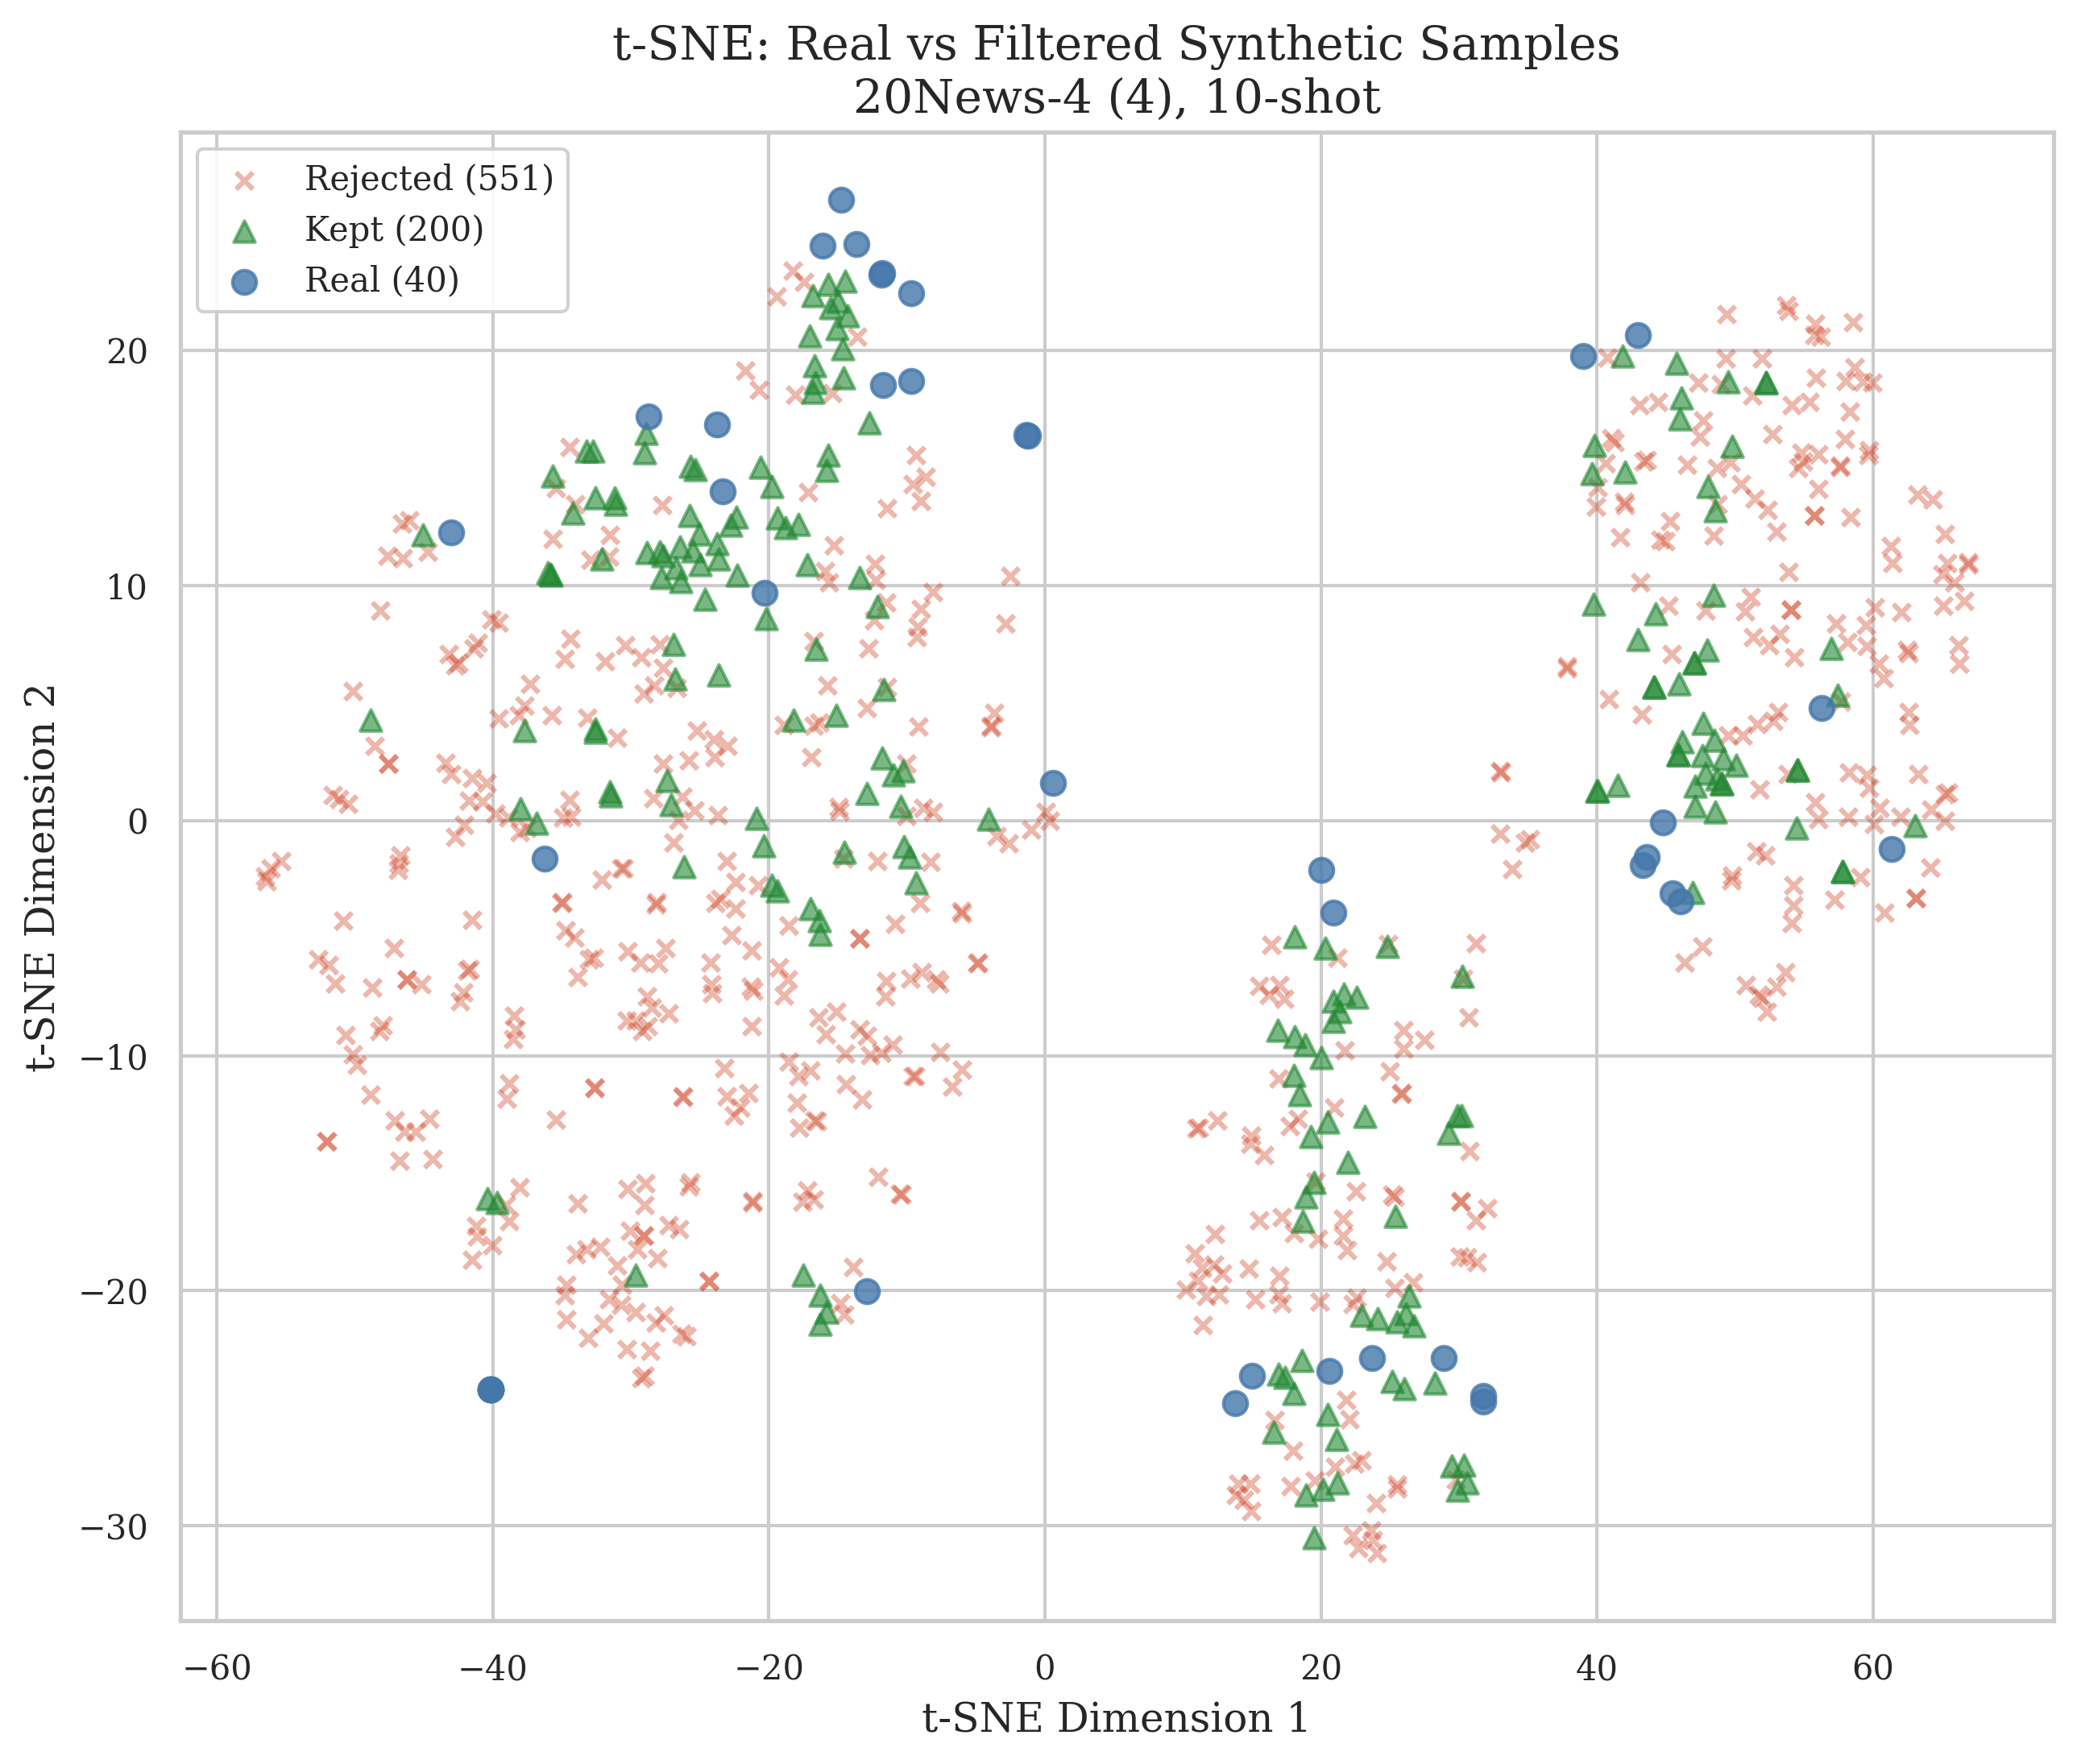
\includegraphics[width=0.85\textwidth]{Figures/fig_tsne_20news.png}
\caption{Proyección t-SNE del espacio de embeddings para 20newsgroups con 10 ejemplos por clase. Las muestras reales (círculos) definen los conglomerados de cada clase. Las muestras filtradas (triángulos) se ubican dentro o cerca de estos conglomerados, mientras que las muestras rechazadas (cruces) aparecen en regiones periféricas o en zonas de solapamiento entre clases.}
\label{fig:tsne_20news}
\end{figure}

\begin{figure}[htbp]
\centering
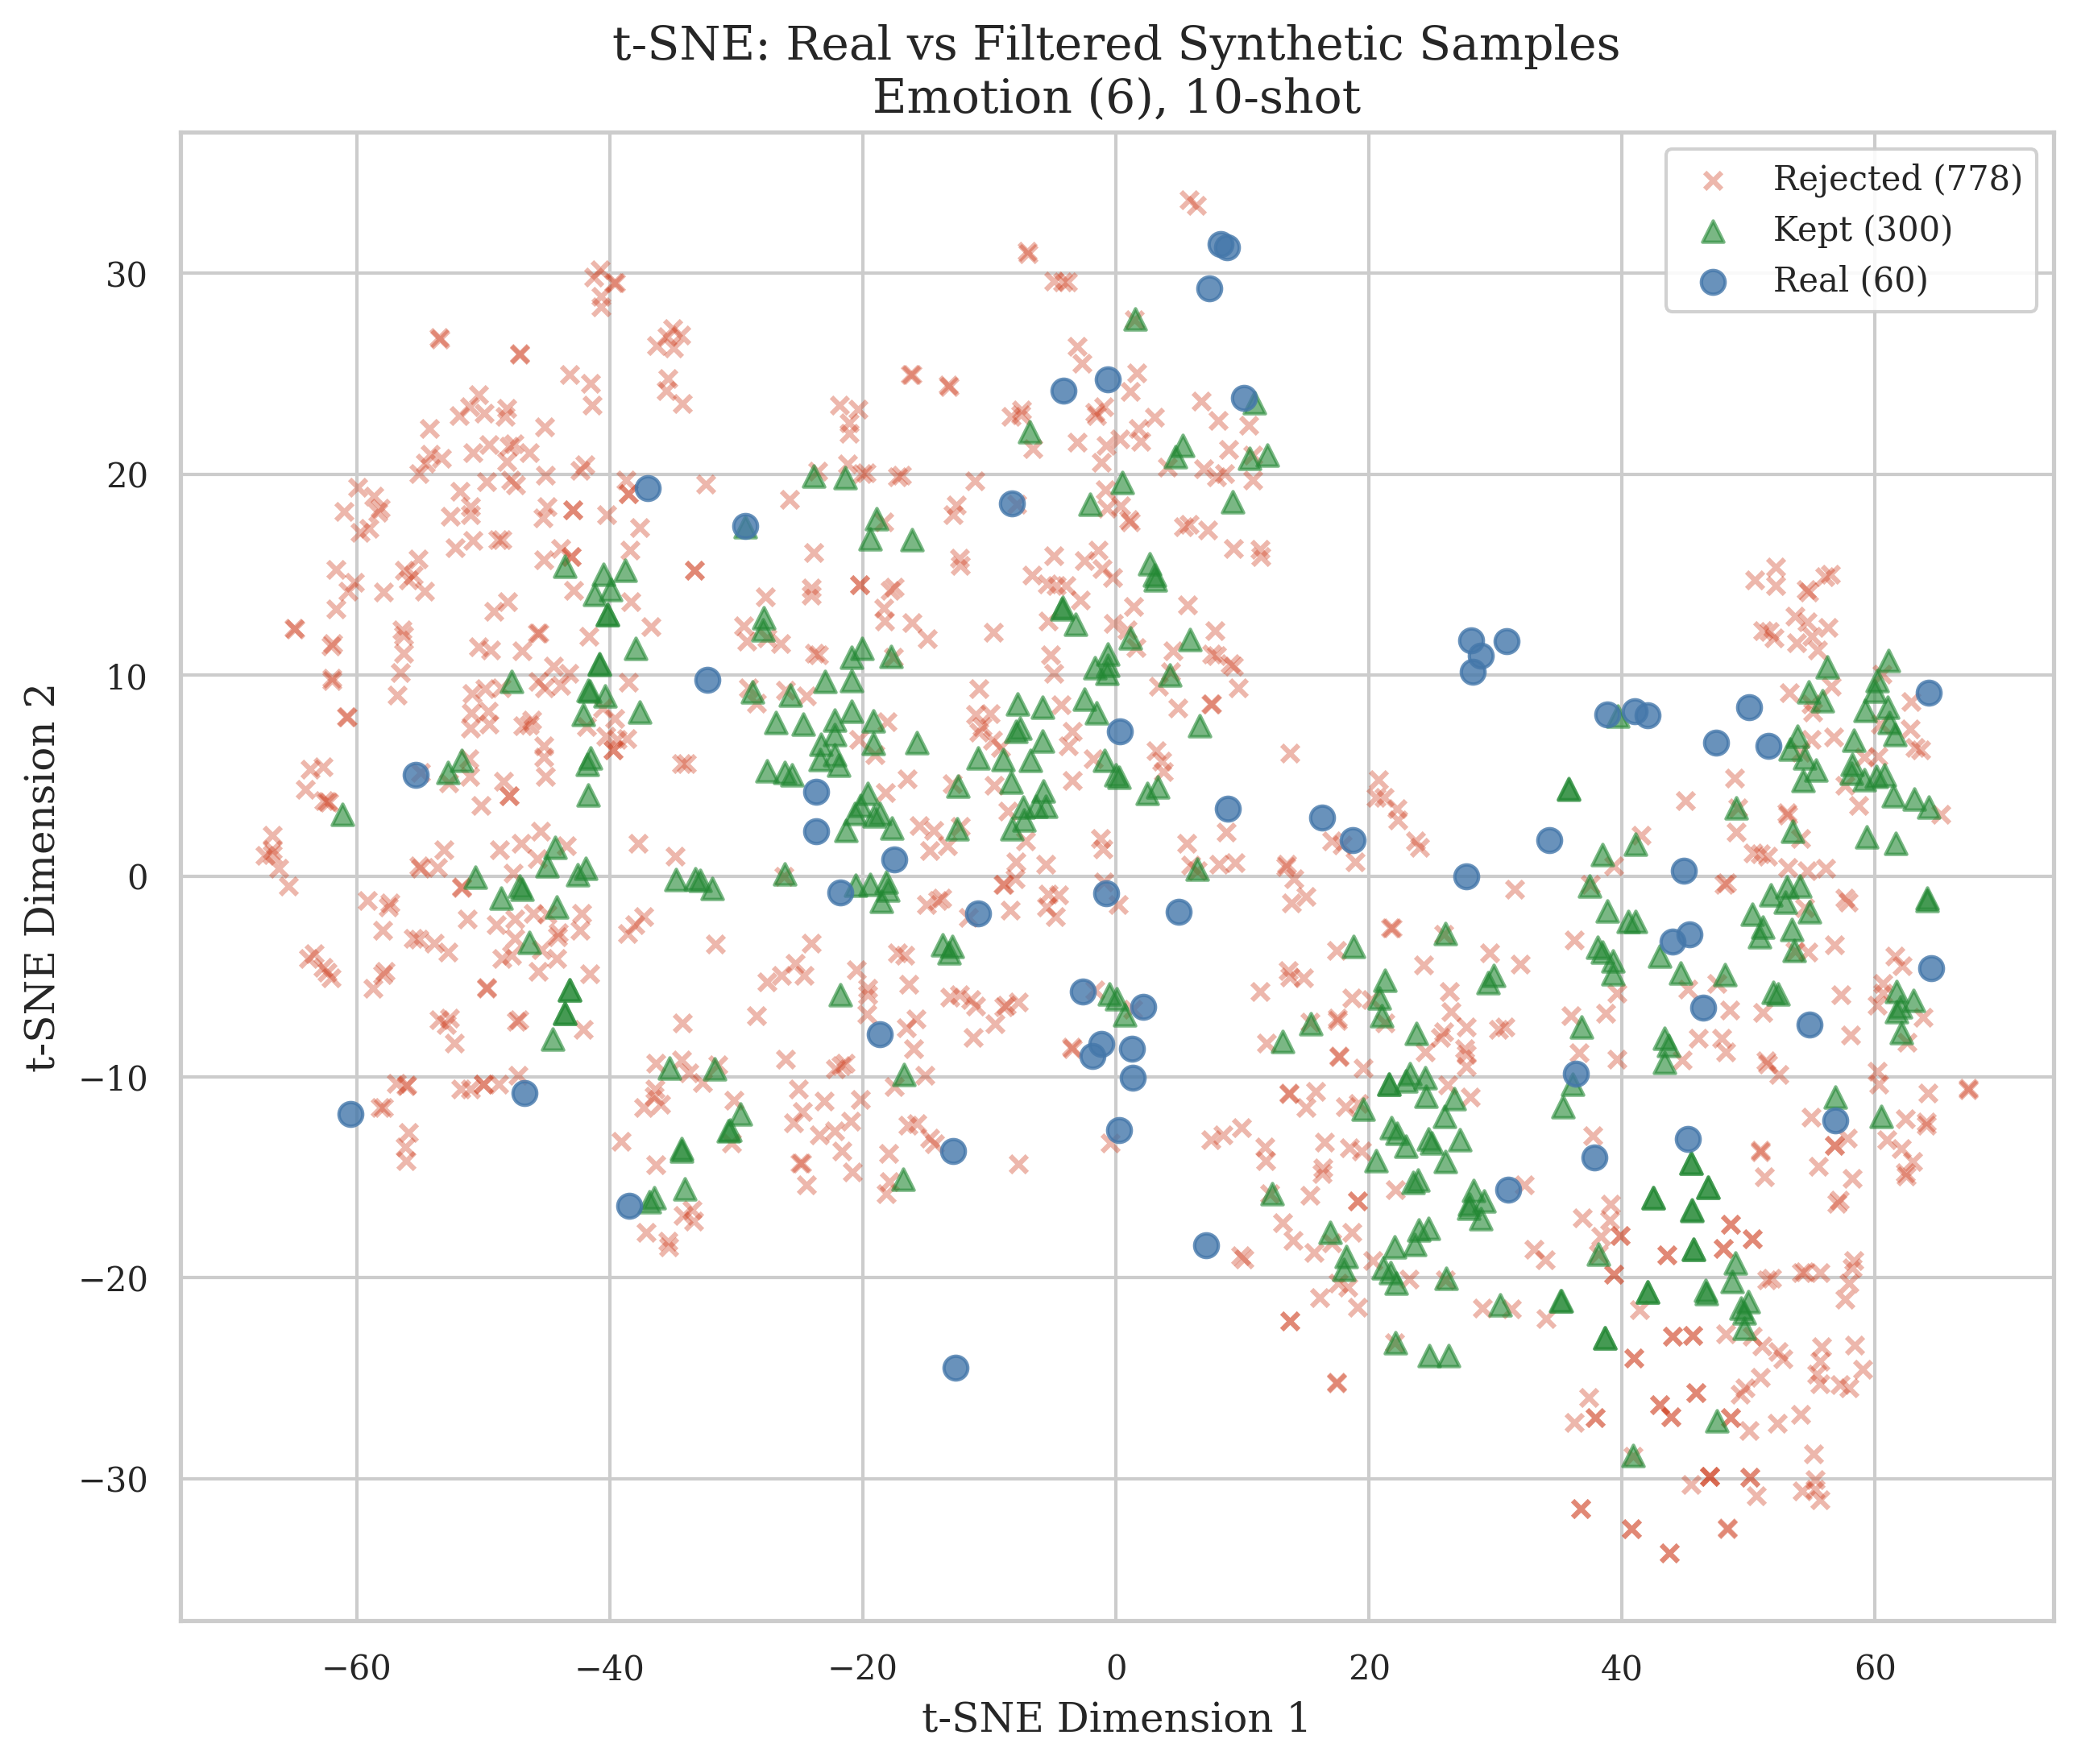
\includegraphics[width=0.85\textwidth]{Figures/fig_tsne_emotion.png}
\caption{Proyección t-SNE para emotion con 10 ejemplos por clase. Las 6 emociones forman conglomerados con diferentes grados de separación. El filtro geométrico selecciona muestras sintéticas que refuerzan los conglomerados existentes sin contaminar regiones de otras clases.}
\label{fig:tsne_emotion}
\end{figure}

\begin{figure}[htbp]
\centering
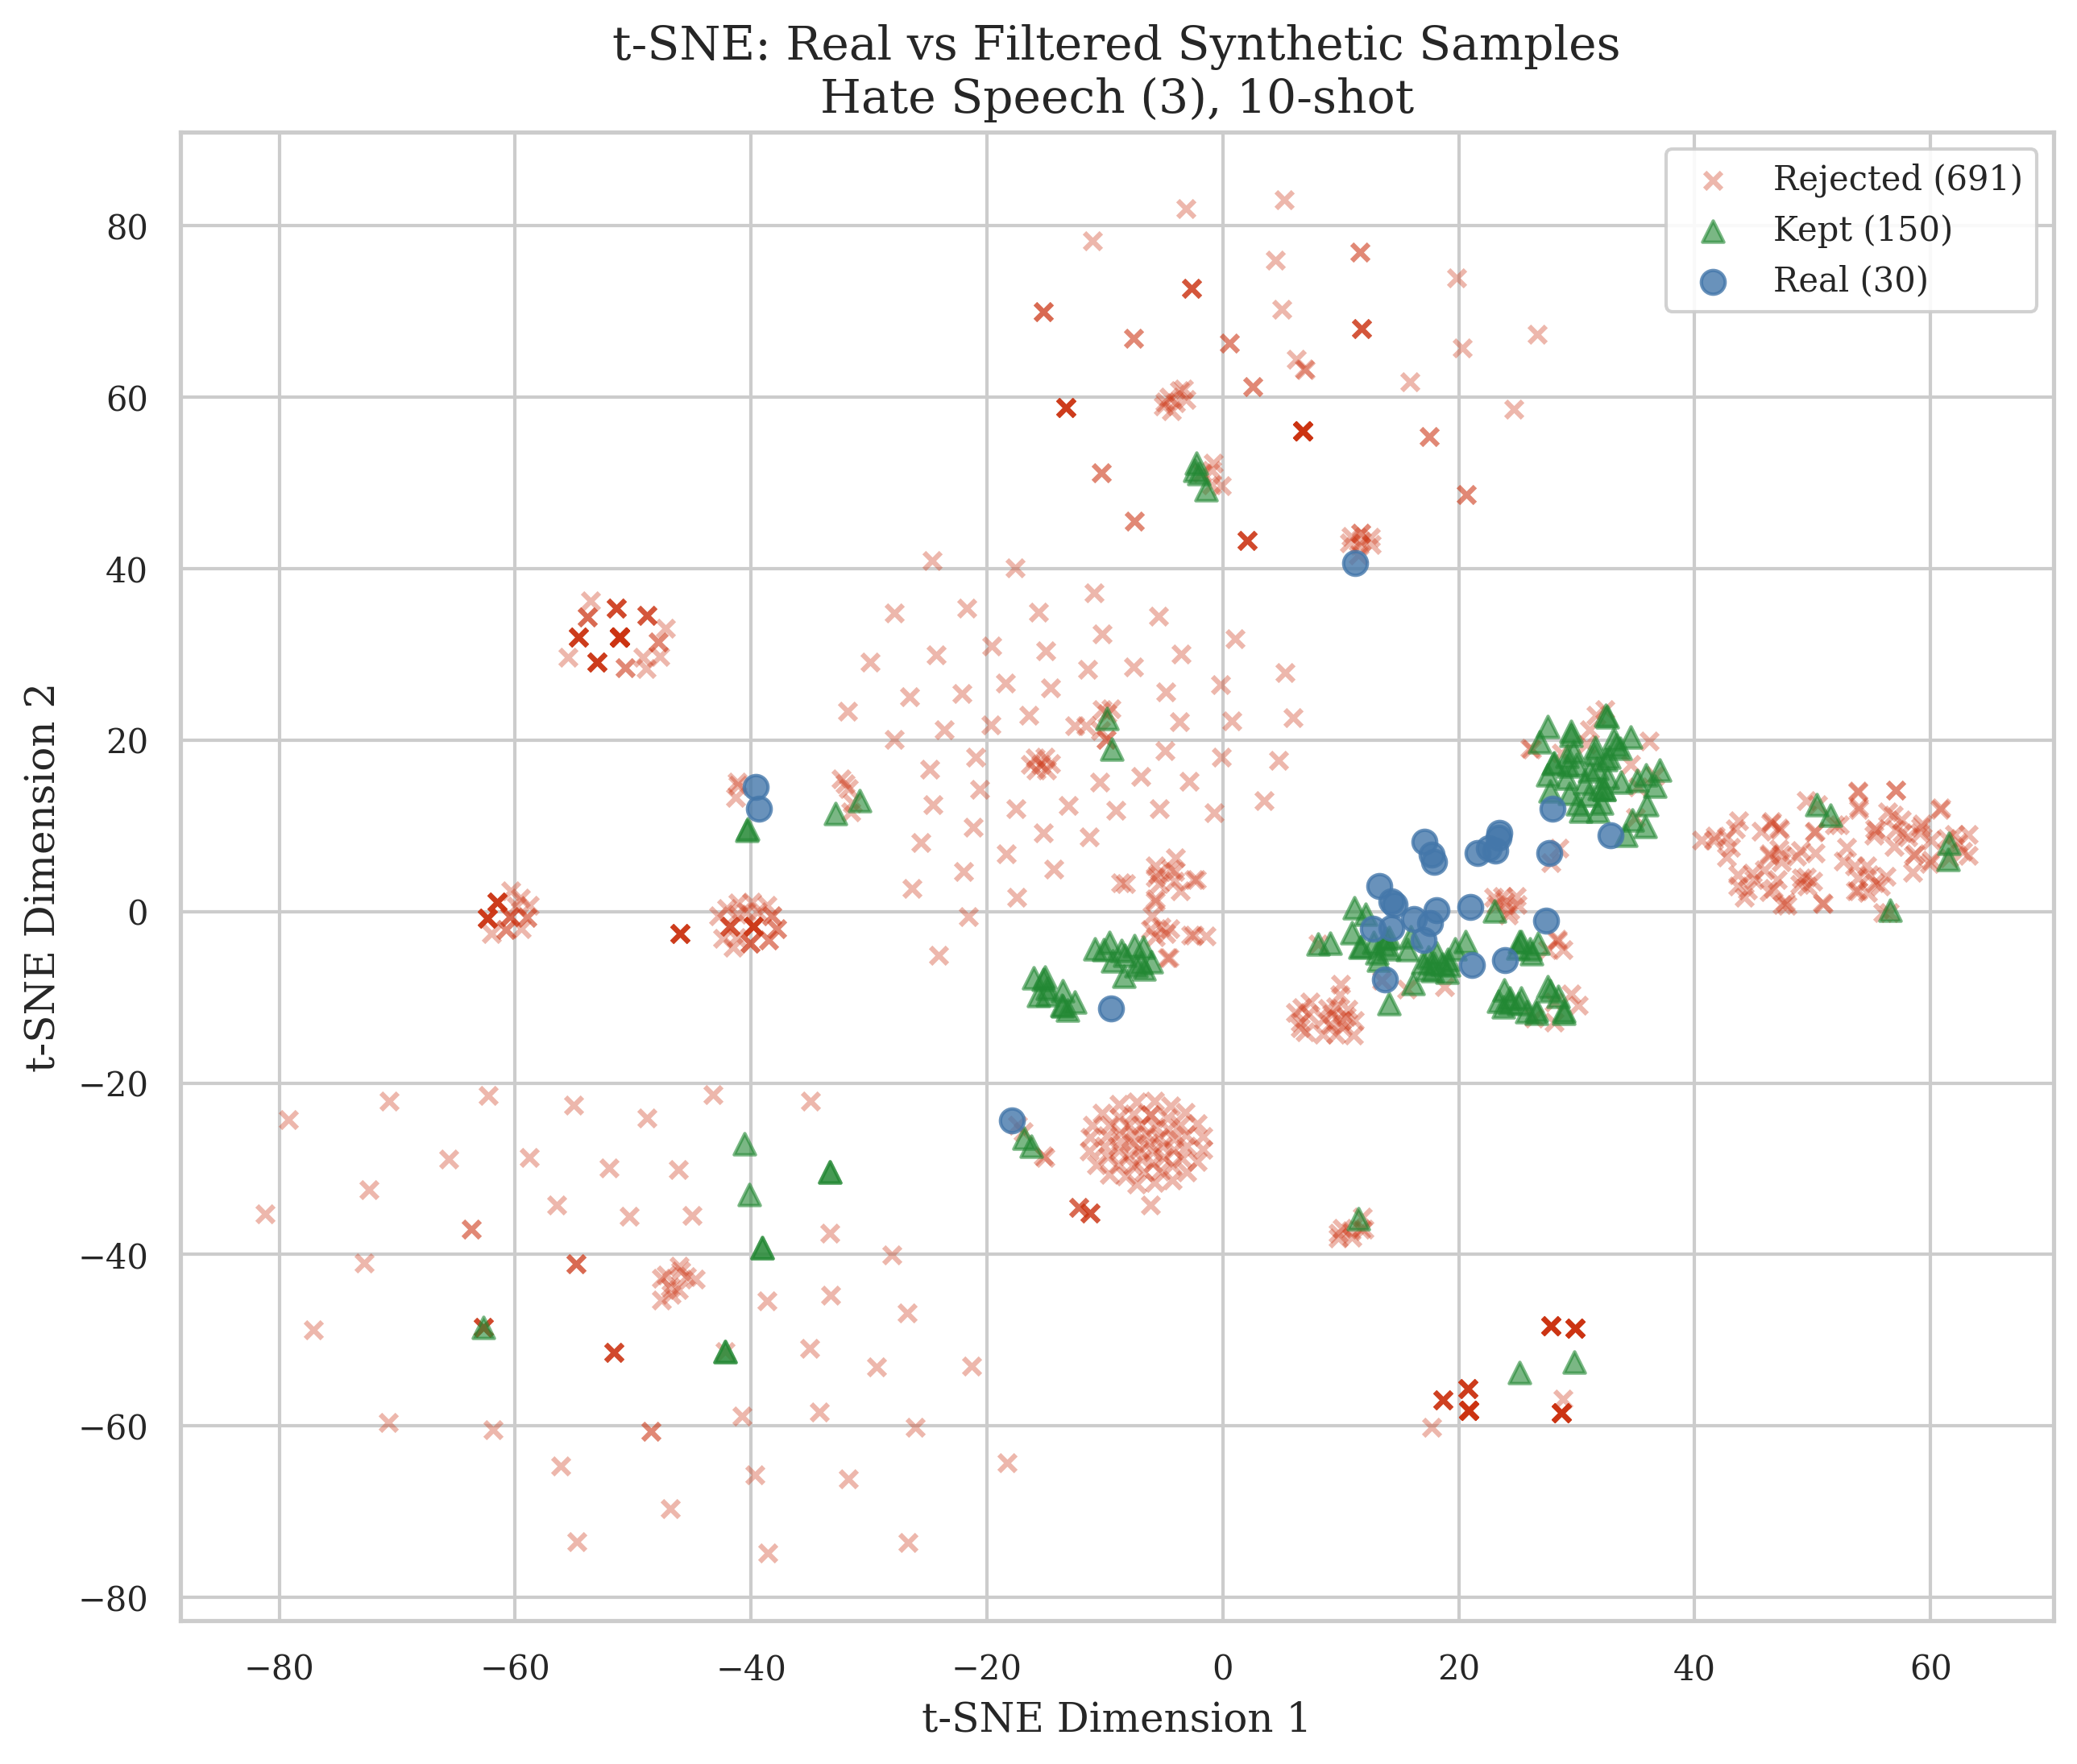
\includegraphics[width=0.85\textwidth]{Figures/fig_tsne_hate_speech.png}
\caption{Proyección t-SNE para hate\_speech\_davidson con 10 ejemplos por clase. Este conjunto presenta mayor solapamiento entre clases. El filtro selecciona preferentemente muestras en regiones donde la clase es dominante, evitando zonas de frontera ambigua.}
\label{fig:tsne_hate_speech}
\end{figure}

Las visualizaciones confirman cualitativamente el mecanismo del filtrado geométrico. Las muestras aceptadas por el filtro se ubican en regiones densas del espacio de embeddings donde la clase es localmente dominante. Las muestras rechazadas tienden a aparecer en 3 patrones: (1) en zonas de frontera entre clases, donde podrían confundir las fronteras de decisión; (2) en regiones periféricas alejadas de la distribución real; y (3) aisladas de cualquier conglomerado, sugiriendo alucinaciones del LLM.

La Figura~\ref{fig:scores_20news} muestra la distribución de puntuaciones del filtro para las muestras aceptadas y rechazadas.

\begin{figure}[htbp]
\centering
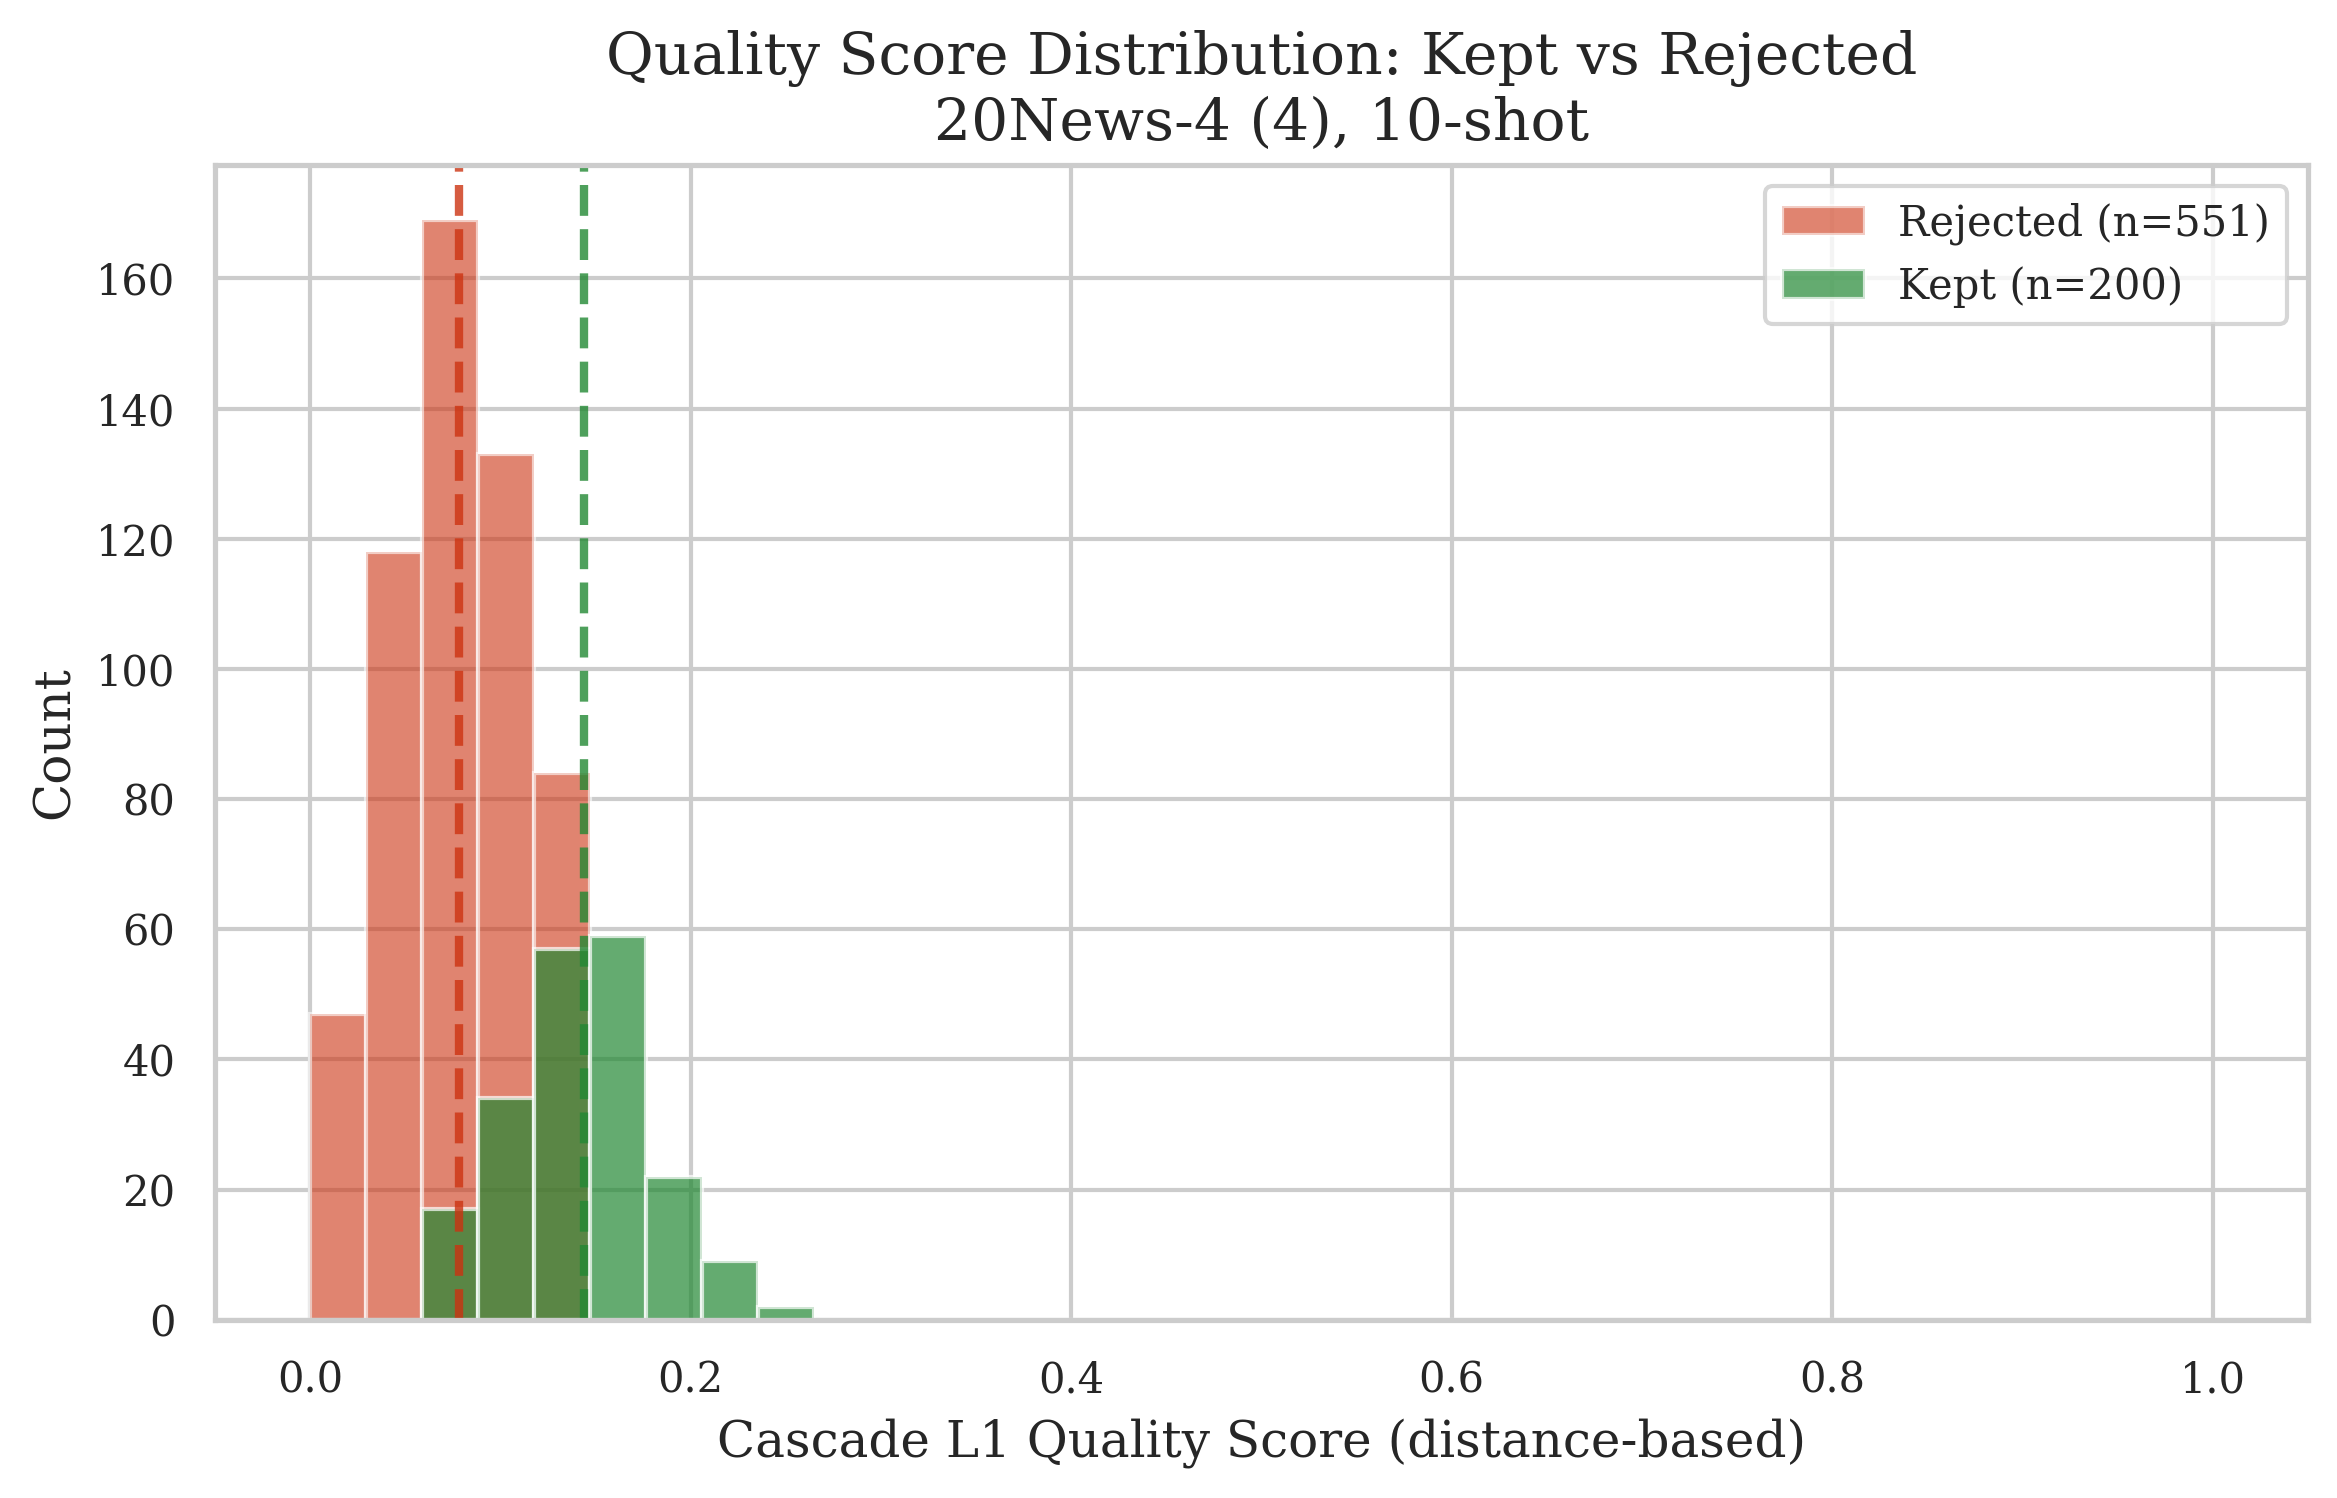
\includegraphics[width=0.85\textwidth]{Figures/fig_scores_20news.png}
\caption{Distribución de puntuaciones del filtro de cascada nivel 1 para 20newsgroups. Las muestras aceptadas (azul) presentan puntuaciones significativamente más altas que las rechazadas (rojo), confirmando la efectividad del criterio de selección basado en distancia.}
\label{fig:scores_20news}
\end{figure}

% Chapter 7 - Conclusiones

\chapter{Conclusiones}
\label{ch:conclusiones}

Este capítulo sintetiza los hallazgos experimentales, evalúa el cumplimiento de las hipótesis planteadas, identifica las contribuciones de la investigación, discute los resultados contraintuitivos, reconoce las limitaciones del estudio, y propone direcciones para trabajo futuro.

\section{Síntesis de Resultados}
\label{sec:sintesis_resultados}

El filtrado geométrico de muestras de texto generadas por modelos de lenguaje de gran escala mejora significativamente la clasificación de texto en escenarios de pocos ejemplos por clase. La evidencia proviene de más de 8,000 configuraciones experimentales evaluadas sobre 13 conjuntos de datos que abarcan 9 dominios textuales, 2 tareas de procesamiento de lenguaje natural y 5 modelos generativos de 4 proveedores distintos.

El resultado más fuerte se obtiene en la comparación con 10 métodos de aumentación sobre 1,890 configuraciones: la ponderación suave alcanza +2.61 puntos porcentuales respecto a SMOTE ($p < 0.0001$ con corrección de Bonferroni, $d = 0.95$, tasa de victoria del 88.9\%). El tamaño de efecto se clasifica como grande. En el experimento principal con 3,675 configuraciones, la mejora es de +2.25 puntos porcentuales ($p < 0.0001$, $d = 0.74$, tasa de victoria del 83.8\%).

El método funciona mejor con 10 a 25 ejemplos por clase, donde las ganancias alcanzan +4.52 y +1.88 puntos porcentuales respectivamente. Con 50 ejemplos, la mejora no alcanza significancia estadística. El rango óptimo de clases es de 2 a 20; con 77 o más clases el filtrado geométrico no aporta mejora.

La extensión a reconocimiento de entidades nombradas produce ganancias de +9.61 puntos porcentuales con tasa de victoria del 100\%, confirmando que los filtros geométricos son agnósticos a la tarea.

La evaluación con 5 modelos generativos (Gemini 3 Flash, GPT-5-mini, Claude 4.5 Haiku, Kimi K2.5, GLM-5) confirma que el método es agnóstico al LLM. Los 5 modelos producen mejoras significativas tras corrección de Bonferroni, con una dispersión de solo 0.82 puntos porcentuales entre el mejor (+2.31) y el peor (+1.49). El test de Friedman no detecta un efecto significativo del modelo generativo ($p = 0.086$), y la correlación inter-LLM ($\tau_K = 0.59$) indica acuerdo sustancial sobre qué configuraciones se benefician más del filtrado.

El análisis por clase individual revela que las clases difíciles (F1 base $<$ 30\%) se benefician desproporcionadamente, con ganancias medias de +10.44 puntos porcentuales, mientras que las clases fáciles (F1 $>$ 80\%) obtienen apenas +0.55 puntos porcentuales. Este patrón indica que el filtrado geométrico aporta mayor valor precisamente donde el clasificador tiene mayor margen de mejora: en las fronteras de decisión más inciertas del espacio de embeddings. En términos de F1 absoluto, la ponderación suave alcanza un macro F1 del 73.49\% frente al 71.24\% de SMOTE, contextualizando la mejora de +2.25 puntos porcentuales como una reducción del 7.8\% del error residual.

El experimento de aprendizaje curricular demuestra que la introducción ordenada de muestras sintéticas por score geométrico mejora el rendimiento respecto a la incorporación simultánea. El pico se alcanza al incluir el 50\% superior de los candidatos (+2.74 puntos porcentuales vs SMOTE, tasa de victoria del 86.2\%), superando al método estándar por +0.66 puntos porcentuales. Aproximadamente la mitad de las muestras generadas introduce ruido que degrada la calidad del clasificador.

La comparación entre filtrado geométrico y filtrado basado en modelo teacher confirma la superioridad del enfoque geométrico. El filtrado geométrico binario alcanza +2.78 puntos porcentuales frente a +2.43 del teacher binario. La diferencia es estadísticamente significativa ($p = 0.0001$), lo que demuestra que la distancia euclidiana al centroide de clase captura información más general que la confianza de un clasificador específico.

Las estadísticas geométricas del espacio de embeddings validan cuantitativamente el mecanismo del filtrado. Las muestras filtradas producen clústeres más compactos (distancia intra-clase: 0.822 vs 0.850 sin filtrar, $p < 0.001$) y mejor separados (distancia inter-clase: 0.616 vs 0.571, $p < 0.001$). El silhouette score mejora de 0.075 a 0.085 ($p = 0.029$), con victoria del filtrado en el 71\% de las configuraciones. Estos resultados confirman que el filtrado no solo selecciona muestras de mayor calidad sino que mejora la estructura geométrica del espacio de representación aumentado.

El experimento de aumentación híbrida adaptativa por clase demuestra que la especialización por dificultad no supera al filtrado geométrico uniforme. El filtrado puro alcanza +2.33 puntos porcentuales ($d = 0.93$, tasa de victoria del 91.0\%), mientras que la mejor estrategia híbrida obtiene solo +0.77 puntos porcentuales. El rendimiento mejora monótonamente a medida que más clases reciben filtrado geométrico en lugar de SMOTE, confirmando que la aplicación uniforme del mejor método es preferible a la especialización.

\section{Validación de Hipótesis}
\label{sec:validacion_hipotesis}

La \textbf{hipótesis principal H1} queda confirmada. El filtrado geométrico produce mejoras estadísticamente significativas respecto a SMOTE y todos los demás métodos de aumentación evaluados. La evidencia satisface los 3 criterios de aceptación: magnitud positiva (+2.25 puntos porcentuales), significancia estadística ($p < 0.0001$ con corrección de Bonferroni), y consistencia (tasa de victoria del 83.8\%).

La \textbf{hipótesis H1a} (filtrado) queda confirmada. El filtrado binario supera a la ausencia de aumentación por +2.08 puntos porcentuales ($p < 0.0001$, $d = 0.65$, tasa de victoria del 80.0\%). La selección geométrica de muestras aporta valor significativo respecto a la incorporación indiscriminada de todas las muestras generadas.

La \textbf{hipótesis H1b} (ponderación suave) queda parcialmente confirmada. En el experimento principal, la diferencia entre ponderación suave y filtrado binario es de +0.13 puntos porcentuales ($p = 0.10$), resultado que no alcanza significancia estadística. El estudio dedicado con hiperparámetros optimizados (normalización min-max, temperatura 0.5, selección top-N) muestra una ganancia de +3.66 puntos porcentuales con tasa de victoria del 84.5\%, pero este resultado representa un techo de rendimiento con configuración óptima, no el caso típico. La contribución principal del sistema propuesto reside en el filtrado geométrico en sí --- la selección de qué muestras incluir --- que produce ganancias estadísticamente significativas independientemente del esquema de ponderación. La ponderación suave aporta una mejora incremental cuya magnitud depende del ajuste de hiperparámetros, lo que limita su utilidad práctica como contribución autónoma.

La \textbf{hipótesis H1c} (generalización entre tareas) queda confirmada. Los filtros geométricos diseñados para clasificación de texto producen +9.61 puntos porcentuales en reconocimiento de entidades nombradas, con tasa de victoria del 100\% sobre 9 configuraciones. La adaptación no requiere modificación de los filtros, solo de la definición de clase.

La \textbf{hipótesis H1d} (efecto del clasificador) queda confirmada. El SVC lineal obtiene +2.98 puntos porcentuales ($d = 1.02$), Ridge +2.74 puntos porcentuales ($d = 1.04$), mientras que el bosque aleatorio obtiene +1.42 puntos porcentuales sin significancia estadística ($p = 0.11$). Los clasificadores lineales aprovechan más efectivamente las muestras filtradas.

\section{Contribuciones}
\label{sec:contribuciones}

Esta investigación aporta 9 contribuciones al campo de la aumentación de datos para clasificación de texto.

La primera contribución es un sistema de filtrado geométrico que selecciona muestras sintéticas de alta calidad en el espacio de embeddings. El sistema opera de manera desacoplada del modelo generativo, lo que se valida empíricamente con 5 LLMs de 4 proveedores distintos (Sección~\ref{sec:robustez_llm}). Un hallazgo relevante es que el filtro más simple (distancia euclidiana, cascada nivel 1) supera a los filtros multi-criterio complejos. El filtro combinado, que exige satisfacer múltiples criterios simultáneamente, produce resultados catastróficos con tasas de aceptación del 0\% en múltiples configuraciones.

La segunda contribución es el mecanismo de ponderación suave, que transforma las puntuaciones del filtro geométrico en pesos de muestra para el clasificador. La ganancia incremental sobre el filtrado binario es modesta en el experimento principal (+0.13 puntos porcentuales, $p = 0.10$), aunque alcanza +3.66 puntos porcentuales bajo configuración optimizada de hiperparámetros. Este resultado establece que la ponderación suave representa una extensión opcional cuyo beneficio depende del ajuste de temperatura y normalización, no un componente esencial del sistema. La contribución conceptual --- utilizar los scores geométricos como señal continua de calidad en lugar de un umbral binario --- permanece válida como dirección de investigación, aun cuando su impacto práctico sea incremental.

La tercera contribución es la validación sobre 10 conjuntos de datos que abarcan 7 dominios textuales distintos, con múltiples semillas aleatorias y corrección estadística rigurosa. La evaluación incluye pruebas t pareadas con corrección de Bonferroni, tamaños de efecto (d de Cohen), intervalos de confianza bootstrap al 95\% y tasas de victoria. El nivel de rigor estadístico supera al estándar habitual en la literatura de aumentación de datos.

La cuarta contribución es la demostración de generalización a reconocimiento de entidades nombradas. Los mismos filtros, sin modificación, producen mejoras de +9.61 puntos porcentuales en NER. Este resultado confirma que el filtrado basado en distancia euclidiana captura propiedades geométricas agnósticas a la tarea.

La quinta contribución es la evidencia comprensiva de que los filtros simples superan a los complejos. Esta observación, consistente a través de clasificación de texto, NER y 4 modelos de embeddings diferentes, constituye un hallazgo práctico relevante para la comunidad: la simplicidad en el diseño del filtro no solo reduce la complejidad de implementación sino que mejora el rendimiento.

La sexta contribución es la demostración de que el beneficio del filtrado geométrico se concentra en las clases más difíciles. El análisis desagregado por clase individual muestra una relación inversa entre el rendimiento base de la clase y la ganancia del filtrado: las clases con F1 inferior al 30\% obtienen ganancias medias de +10.44 puntos porcentuales, mientras que las clases con F1 superior al 80\% obtienen +0.55 puntos porcentuales. Este hallazgo tiene implicaciones prácticas directas: el filtrado geométrico es especialmente valioso para sistemas donde el rendimiento en clases difíciles o minoritarias es crítico.

La séptima contribución es la demostración mediante aprendizaje curricular de que la cantidad óptima de muestras sintéticas es inferior al total de candidatos disponibles. El rendimiento alcanza su pico al incluir el 50\% superior de los candidatos ordenados por score geométrico, con una ganancia de +0.66 puntos porcentuales sobre la incorporación simultánea de todos los candidatos. Este resultado proporciona una guía práctica para calibrar el presupuesto de muestras sintéticas y confirma que la calidad de la selección prevalece sobre la cantidad.

La octava contribución es la evidencia experimental de que la aplicación uniforme del filtrado geométrico supera a las estrategias híbridas adaptativas por clase. A pesar de que las clases difíciles se benefician desproporcionadamente del filtrado, especializar el método de aumentación por dificultad estimada degrada el rendimiento global. Este resultado, evaluado sobre 1,323 configuraciones con 3 métodos de estimación de dificultad, demuestra que la robustez del filtrado geométrico a través de todas las clases es preferible a la optimización local por subgrupos.

La novena contribución es la validación empírica de la independencia del modelo generativo. La evaluación con 5 LLMs de 4 proveedores (Gemini 3 Flash, GPT-5-mini, Claude 4.5 Haiku, Kimi K2.5, GLM-5) demuestra que el filtrado geométrico produce mejoras significativas independientemente del modelo utilizado. El test de Friedman ($p = 0.086$) no detecta diferencias significativas entre modelos, y la correlación inter-LLM ($\tau_K = 0.59$) confirma acuerdo sustancial. Este resultado transforma la afirmación de desacoplamiento, de un argumento de diseño a una evidencia empírica.

\section{Hallazgos Contraintuitivos}
\label{sec:hallazgos_contraintuitivos}

Cuatro resultados de esta investigación contradicen expectativas previas de la literatura.

El primer hallazgo contraintuitivo es que los filtros simples superan a los complejos. La cascada nivel 1 (solo distancia euclidiana) supera consistentemente al filtro combinado multi-criterio. Este último produce tasas de aceptación del 0\% en múltiples configuraciones, tanto en clasificación de texto como en NER. La Sección~\ref{sec:analisis_complejidad} desarrolla tres mecanismos que explican este resultado: la correlación matemática entre métricas en espacios normalizados (la distancia euclidiana y la similitud coseno producen rankings idénticos para vectores unitarios), la reducción de diversidad por intersección restrictiva de criterios, y la inestabilidad de las métricas de densidad local en el régimen de pocos ejemplos. Este análisis encuentra sustento teórico en Robinson et al. \cite{robinson2025manifold} y Du et al. \cite{du2025disentangling}. La simplicidad resulta ser una virtud, no una limitación.

El segundo hallazgo es que todas las líneas base modernas pierden contra SMOTE. La paráfrasis con T5, la aumentación contextual con BERT y el mixup en embeddings obtienen resultados negativos respecto a SMOTE simple. A pesar de su mayor sofisticación computacional y su uso de modelos preentrenados de gran escala, estas técnicas no generan diversidad genuina en el espacio de representación. Este resultado cuestiona la narrativa predominante de que las técnicas basadas en modelos preentrenados superan automáticamente a los métodos clásicos.

El tercer hallazgo es que la mejora iterativa del prompt no mejora las tasas de aceptación. El sistema de retroalimentación que analiza los motivos de rechazo y modifica el prompt en consecuencia produce tasas de aceptación decrecientes a lo largo de las iteraciones ($-12.3$ puntos porcentuales entre la iteración 0 y la 4). El cuello de botella no reside en la calidad del prompt sino en propiedades inherentes de la generación del LLM para ciertas distribuciones.

El cuarto hallazgo es que la especialización por dificultad de clase no mejora sobre la aplicación uniforme del filtrado geométrico. A pesar de que las clases difíciles obtienen ganancias 19 veces mayores que las fáciles (+10.44 vs +0.55 puntos porcentuales), reemplazar el filtrado geométrico por SMOTE en las clases fáciles degrada el rendimiento global. La mejor estrategia híbrida (+0.77 puntos porcentuales) queda muy por debajo del filtrado puro (+2.33 puntos porcentuales). El rendimiento mejora monótonamente con la proporción de clases que reciben filtrado geométrico, lo que indica que incluso las ganancias modestas en clases fáciles contribuyen al rendimiento agregado.

\section{Limitaciones}
\label{sec:limitaciones}

Esta investigación presenta varias limitaciones que delimitan el alcance de sus conclusiones.

La evaluación se realiza exclusivamente en inglés. El rendimiento del filtrado geométrico en otros idiomas no fue evaluado. Idiomas con menor representación en los modelos de embeddings podrían producir espacios de representación con propiedades geométricas diferentes.

La investigación utiliza un modelo principal de embeddings (all-mpnet-base-v2 de 768 dimensiones). Aunque la ablación con 4 modelos demuestra robustez (90.5\% de acuerdo mayoritario), todos los modelos pertenecen a la familia de transformers para inglés.

Existe una circularidad entre el espacio de filtrado y el de clasificación: el mismo modelo de embeddings se utiliza para calcular las distancias geométricas que determinan qué muestras se seleccionan y como representación de entrada para los clasificadores. Esto implica que el filtro optimiza la posición de las muestras en el mismo espacio donde el clasificador las evalúa, lo que podría favorecer artificialmente al filtrado geométrico. Tres líneas de evidencia mitigan esta preocupación. Primera, la ablación con 4 modelos de embeddings demuestra que cuando el filtrado se realiza con un modelo diferente al utilizado para clasificación, el acuerdo entre modelos es del 90.5\% (19 de 21 configuraciones), indicando que la selección geométrica captura propiedades de calidad que no son específicas del espacio de representación. Segunda, el filtrado geométrico iguala o supera al filtrado basado en modelo teacher, que utiliza un clasificador separado para evaluar la confianza de cada muestra. Tercera, los filtros generalizan a NER, donde la evaluación final emplea SpaCy y métricas seqeval a nivel de entidad, un pipeline completamente independiente del modelo de embeddings. No obstante, un diseño experimental ideal emplearía modelos de embeddings diferentes para filtrado y clasificación de manera sistemática. El 9.5\% de configuraciones sin acuerdo entre modelos (correspondientes a escenarios de 50 ejemplos, donde la aumentación aporta menos valor) sugiere que la circularidad podría tener efectos marginales en ciertos regímenes.

La evaluación multi-LLM emplea 5 modelos, todos de la generación más reciente de modelos comerciales. No se evalúan modelos de código abierto ejecutados localmente (como Llama o Mistral), donde la calidad de generación podría diferir. Adicionalmente, los filtros de contenido de los modelos evaluados impiden la generación para clases sensibles (discurso de odio, contenido religioso), lo que limita la aplicabilidad del método en dominios que involucren contenido potencialmente ofensivo. La clase ``hate\_speech'' fue rechazada por los 5 modelos en al menos una configuración.

Las generaciones del LLM se almacenan en caché, lo que produce varianza cero entre semillas para clasificadores determinísticos. El 80\% de las combinaciones método/clasificador presentan esta característica. Los intervalos de confianza podrían subestimar la varianza real que se observaría con regeneración completa de muestras en cada semilla. Restringiendo el análisis a clasificadores estocásticos, el resultado sigue siendo significativo (+1.79 puntos porcentuales, $p = 0.0015$, $d = 0.52$). Este análisis de sensibilidad constituye la prueba más conservadora de las hipótesis de esta investigación. Un diseño experimental alternativo regeneraría las muestras sintéticas con diferentes prompts o temperaturas del LLM en cada semilla, proporcionando una estimación más fiel de la variabilidad real. La significancia del resultado con clasificadores estocásticos ($d = 0.52$, efecto mediano) sugiere que las conclusiones son robustas, pero los intervalos de confianza del análisis completo deben interpretarse como cotas inferiores de la incertidumbre real.

El resultado a 50 ejemplos por clase no alcanza significancia estadística ($p = 0.16$). El método es más valioso en escenarios de recursos limitados (10-25 ejemplos). Con datos de entrenamiento moderados, la aumentación aporta valor marginal decreciente.

La evaluación de NER emplea SpaCy como modelo de reconocimiento de entidades. Los modelos de NER de última generación podrían producir resultados diferentes. La elección de SpaCy responde a su reproducibilidad y disponibilidad, pero limita la comparabilidad con la literatura más reciente de NER.

El número de clases limita las ganancias. Con 77 clases (banking77) el resultado es negativo ($-0.99$ puntos porcentuales) y con 150 clases (clinc150) es neutro (+0.01 puntos porcentuales). El filtrado geométrico basado en distancia pierde efectividad cuando el espacio de embeddings se fragmenta excesivamente.

\section{Trabajo Futuro}
\label{sec:trabajo_futuro}

La extensión multilingüe representa la dirección más inmediata. Evaluar el filtrado geométrico sobre modelos de embeddings multilingües permitiría verificar si las propiedades geométricas que fundamentan el filtrado se mantienen en otros idiomas.

La evaluación con modelos generativos de código abierto ejecutados localmente constituye una segunda línea prioritaria. La validación multi-LLM de esta investigación emplea modelos comerciales con API; evaluar modelos como Llama y Mistral ejecutados sin filtros de contenido permitiría verificar si el método funciona en dominios sensibles donde los modelos comerciales rechazan la generación.

La búsqueda conjunta de hiperparámetros mediante optimización bayesiana podría revelar configuraciones superiores. La optimización secuencial utilizada en esta investigación explora cada parámetro independientemente. Una búsqueda conjunta capturaría interacciones entre el modelo de embeddings, el nivel de filtrado, la temperatura de ponderación y el número de candidatos generados.

La selección adaptativa de temperatura por clase ofrece potencial de mejora. Clases con alta variabilidad interna podrían beneficiarse de temperaturas más altas en la generación, mientras que clases compactas podrían preferir generaciones más conservadoras.

El presupuesto adaptativo de generación por clase asignaría más recursos a clases difíciles. En lugar de generar el mismo número de candidatos para cada clase, un sistema adaptativo invertiría más en las clases con menor tasa de aceptación o mayor dificultad de clasificación.

La estimación formal de ratios de densidad permitiría formalizar el muestreo por importancia que subyace a la ponderación suave. Una estimación explícita de la relación entre la distribución de generación del LLM y la distribución real de cada clase proporcionaría pesos más fundamentados teóricamente.

La extensión a otras tareas de procesamiento de lenguaje natural, como generación de preguntas, resumen extractivo y traducción automática, verificaría el alcance de la generalización demostrada en esta investigación entre clasificación y NER.


\newpage
%\bibliographystyle{ieeetr}
\bibliographystyle{apacite} %Para estilo APA, comentar la otra línea
\bibliography{citas}

%----------------------------------------------------------------------------------------
%	THESIS CONTENT - APPENDICES
%----------------------------------------------------------------------------------------

\appendix % Cue to tell LaTeX that the following "chapters" are Appendices

% Include the appendices of the thesis as separate files from the Appendices folder
% Uncomment the lines as you write the Appendices

% Appendix A - Validaciones Metodológicas

\chapter{Validaciones Metodológicas}
\label{ch:appendix_validaciones}

\section{Validación de la Implementación de SMOTE}
\label{sec:validacion_smote}

La Tabla~\ref{tab:smote_validation} presenta la comparación entre la implementación \textit{dummy-binary} utilizada en esta investigación (que crea un problema binario auxiliar por clase con ruido gaussiano como clase ficticia) y la implementación estándar multiclase de SMOTE (que utiliza máscara binaria objetivo vs resto). Ambas implementaciones invocan internamente el algoritmo \texttt{SMOTE} de la biblioteca \texttt{imbalanced-learn}.

\begin{table}[htbp]
\centering
\caption{Validación de la implementación de SMOTE: por clase (\textit{dummy-binary}) vs estándar multiclase. Macro F1 con regresión logística sobre las 9 combinaciones conjunto $\times$ semilla. Las dos columnas son idénticas porque, fijada la semilla, ambas implementaciones invocan el mismo algoritmo \texttt{imblearn.SMOTE} con los mismos $k$-vecinos intra-clase, generando muestras sintéticas bit-a-bit idénticas.}
\label{tab:smote_validation}
\small
\setlength{\tabcolsep}{4pt}
\begin{tabular}{llrrr}
\toprule
\textbf{Conjunto} & \textbf{Sem.} & \textbf{F1 \textit{dummy}} & \textbf{F1 multic.} & \textbf{$|\Delta|$ (pp)} \\
\midrule
sms\_spam\_10shot              & 42  & 0.8683 & 0.8683 & 0.0000 \\
                               & 123 & 0.8853 & 0.8853 & 0.0000 \\
                               & 456 & 0.8742 & 0.8742 & 0.0000 \\
\midrule
20newsgroups\_10shot           & 42  & 0.7493 & 0.7493 & 0.0000 \\
                               & 123 & 0.7396 & 0.7396 & 0.0000 \\
                               & 456 & 0.7409 & 0.7409 & 0.0000 \\
\midrule
hate\_speech\_davidson\_10shot & 42  & 0.5249 & 0.5249 & 0.0000 \\
                               & 123 & 0.5271 & 0.5271 & 0.0000 \\
                               & 456 & 0.5298 & 0.5298 & 0.0000 \\
\midrule
\multicolumn{2}{l}{\textbf{Total} (27 comparaciones, 3 clasificadores: LR, SVC, Ridge)} & \multicolumn{2}{r}{$|\Delta|$ máximo:} & \textbf{0.0000} \\
\midrule
\multicolumn{5}{l}{\small Umbral de validación: $|\Delta| < 0.1$ pp. \textbf{Resultado: validado.}} \\
\bottomrule
\end{tabular}
\end{table}


La diferencia máxima entre ambas implementaciones es exactamente $0.0000$ puntos porcentuales en las 27 comparaciones realizadas. Este resultado, que a primera vista podría parecer inverosímil, es matemáticamente esperado: con \texttt{random\_state} fijo, el algoritmo SMOTE de \texttt{imbalanced-learn} aplica $k$-vecinos más cercanos exclusivamente sobre las muestras de la clase objetivo. Como en ambas implementaciones el conjunto de embeddings reales de la clase es idéntico, la búsqueda de vecinos produce los mismos pares y los puntos aleatorios de interpolación son idénticos al estar inicializados por la misma semilla. La consecuencia es que las muestras sintéticas generadas son bit-a-bit idénticas, lo que produce conjuntos de entrenamiento aumentados idénticos y, por tanto, clasificadores deterministas con $F1$ idénticos. Cualquier diferencia distinta de cero indicaría un error en la implementación. Este resultado confirma que las ganancias reportadas en esta investigación no se deben a una línea base artificialmente débil.

\section{Análisis de Asimetría de Semillas}
\label{sec:asimetria_semillas}

La Tabla~\ref{tab:seed_asymmetry} presenta el análisis de varianza entre semillas.

\begin{table}[htbp]
\centering
\caption{Impacto de la asimetría de semillas en las pruebas estadísticas (pond. suave vs SMOTE)}
\label{tab:seed_asymmetry}
\small
\begin{tabular}{lrrrrrr}
\toprule
\textbf{Subconjunto} & \textbf{$N$ pares} & \textbf{$\bar{\Delta}$ (pp)} & \textbf{$t$} & \textbf{$p$} & \textbf{$d$ de Cohen} & \textbf{Vic.\%} \\
\midrule
Todos los clasif.       & 105 & +2.25 & 7.63  & $<$0.0001 & 0.745 & 83.8\% \\
Solo estocásticos (MLP+RF)  & 42  & +1.79 & 3.39  & 0.0015    & 0.523 & 78.6\% \\
Determinísticos (LR+SVC+Ridge) & 63  & +2.55 & 7.49  & $<$0.0001 & 0.943 & 87.3\% \\
\midrule
\multicolumn{7}{l}{\small 80\% de los grupos LLM + clasificador determinístico tienen varianza cero entre semillas.} \\
\multicolumn{7}{l}{\small \textbf{El resultado sigue siendo significativo con solo clasificadores estocásticos} ($p=0.0015$).} \\
\bottomrule
\end{tabular}
\end{table}


Las generaciones del LLM se almacenan en caché mediante hash MD5 del prompt. Cuando el mismo prompt se ejecuta con diferentes semillas de muestreo de datos pero el mismo contenido de clase, la caché devuelve respuestas idénticas. Esto produce varianza cero entre semillas para clasificadores determinísticos (regresión logística, SVC, Ridge). El 80\% de las combinaciones LLM + clasificador determinístico presentan esta característica.

Restringiendo el análisis exclusivamente a clasificadores estocásticos (MLP y bosque aleatorio), la ponderación suave mantiene una mejora de +1.79 puntos porcentuales ($p = 0.0015$, $d = 0.52$). El resultado sigue siendo estadísticamente significativo con un tamaño de efecto mediano.

Las pruebas t pareadas siguen siendo válidas porque comparan pares de configuraciones (método vs SMOTE) bajo las mismas condiciones. Los intervalos de confianza podrían subestimar la varianza real al no capturar la variabilidad que introduciría la regeneración de muestras sintéticas con diferentes prompts. Esta limitación se reconoce explícitamente y se discute en el Capítulo~\ref{ch:conclusiones}.

% Appendix B - Experimentos Complementarios

\chapter{Experimentos Complementarios}
\label{ch:appendix_complementarios}

\section{Mejora Iterativa de Prompts}
\label{sec:mejora_iterativa}

Las Tablas~\ref{tab:closed_loop_summary} y \ref{tab:closed_loop_convergence} presentan los resultados del experimento de mejora iterativa.

\begin{table}[htbp]
\centering
\caption{Mejora iterativa de prompts: resumen de rendimiento}
\label{tab:closed_loop_summary}
\begin{tabular}{lrrrr}
\toprule
\textbf{Comparación} & \textbf{$\bar{\Delta}$ (pp)} & \textbf{Vic.\%} & \textbf{Valor $p$} & \textbf{$d$ de Cohen} \\
\midrule
Iterativo vs SMOTE         & +1.12 & 51.7\% & 0.0001 & 0.360 \\
Iterativo vs pasada única  & +2.08 & 40.8\% & 0.0021 & 0.287 \\
\midrule
\multicolumn{5}{l}{\small $N=120$ experimentos. 2 filtros (cascada nivel 1, LOF) $\times$ 5 semillas $\times$ 12 conjuntos.} \\
\multicolumn{5}{l}{\small Ambas comparaciones significativas, pero el filtrado de pasada única es competitivo.} \\
\bottomrule
\end{tabular}
\end{table}


El enfoque iterativo produce +1.12 puntos porcentuales respecto a SMOTE ($p = 0.0001$, $d = 0.36$, tasa de victoria del 52\%). Comparado con el filtrado de pasada única, la mejora iterativa obtiene +2.08 puntos porcentuales ($p = 0.002$, $d = 0.29$, tasa de victoria del 41\%).

\begin{table}[htbp]
\centering
\caption{Convergencia y modos de fallo del ciclo iterativo}
\label{tab:closed_loop_convergence}
\begin{tabular}{llr}
\toprule
\textbf{Categoría} & \textbf{Tipo} & \textbf{Porcentaje} \\
\midrule
\multirow{3}{*}{Razón de convergencia}
 & Objetivo alcanzado     & 62.1\% \\
 & Máximo de iteraciones  & 21.0\% \\
 & Meseta de aceptación   & 16.9\% \\
\midrule
\multirow{2}{*}{Modo de rechazo}
 & Outlier por distancia   & 77.1\% \\
 & Contaminación de clase  & 22.9\% \\
\midrule
\multicolumn{3}{l}{\small Iteraciones promedio por clase: 3.82 (mediana: 4, rango: 2--5)} \\
\multicolumn{3}{l}{\small Tasa de aceptación: 71.2\% (iter. 0) $\to$ 58.9\% (iter. 4): $-$12.3pp} \\
\bottomrule
\end{tabular}
\end{table}


Las tasas de aceptación no mejoran con las iteraciones. La tasa de aceptación promedio disminuye 12.3 puntos porcentuales entre la iteración 0 y la iteración 4. Los modos de fallo dominantes son DISTANCE\_OUTLIER (77\% de los rechazos) y CROSS\_CLASS (23\%). Estos patrones sugieren que las limitaciones provienen de la naturaleza inherente del LLM para ciertas distribuciones, no de la calidad del prompt.

La conclusión es que el filtrado de pasada única es competitivo con la mejora iterativa del prompt. El esfuerzo computacional adicional de múltiples iteraciones no produce ganancias proporcionales. Este hallazgo refuerza la idea de que el cuello de botella no está en la calidad del prompt sino en las propiedades fundamentales de la generación del LLM. La generación progresiva con retroalimentación ha demostrado ser efectiva en otros contextos \cite{ye2022progen}, lo que sugiere que la señal de retroalimentación geométrica podría no ser suficientemente informativa para guiar la mejora del prompt.

\section{Filtrado Geométrico vs. Filtrado Basado en Modelo}
\label{sec:teacher_comparison}

Este experimento compara el filtrado geométrico (basado en distancia euclidiana al centroide de clase) con un filtrado basado en la confianza de un modelo teacher. El modelo teacher es una regresión logística entrenada exclusivamente con datos reales. Para cada muestra sintética, el teacher asigna una probabilidad de pertenencia a la clase correcta. Se comparan 5 métodos: filtrado geométrico binario, filtrado geométrico con ponderación suave, filtrado por confianza del teacher (binario), filtrado por confianza del teacher con ponderación suave, y SMOTE. El diseño comprende 630 evaluaciones: 21 configuraciones de dataset $\times$ 2 clasificadores de evaluación (SVC lineal y Ridge) $\times$ 5 métodos $\times$ 3 semillas. Los clasificadores de evaluación son diferentes del teacher (regresión logística) para evitar circularidad.

La Tabla~\ref{tab:teacher_vs_geometric} presenta la comparación.

\begin{table}[htbp]
\centering
\small
\caption{Comparación entre filtrado geométrico y filtrado basado en modelo teacher. El teacher es una regresión logística entrenada exclusivamente con datos reales. Los clasificadores de evaluación son SVC lineal y Ridge (distintos del teacher).}
\label{tab:teacher_vs_geometric}
\begin{tabular}{lcccccc}
\toprule
\textbf{Método} & \textbf{F1 Macro} & \textbf{$\Delta$ vs SMOTE} & \textbf{IC 95\%} & \textbf{$d$} & \textbf{Victoria} & \textbf{$p$} \\
\midrule
SMOTE & 72.23 & --- & --- & --- & --- & --- \\
Geométrico (binario) & 75.01 & +2.78*** & [2.30, 3.30] & 0.97 & 88.1\% & $<$0.001 \\
Geométrico (ponderado) & 74.70 & +2.46*** & [2.06, 2.88] & 1.05 & 96.0\% & $<$0.001 \\
Teacher (binario) & 74.66 & +2.43*** & [1.98, 2.89] & 0.94 & 88.9\% & $<$0.001 \\
Teacher (ponderado) & 74.38 & +2.15*** & [1.77, 2.54] & 0.98 & 89.7\% & $<$0.001 \\
\midrule
\multicolumn{7}{l}{\small Geométrico vs Teacher (ponderado): $\Delta$ = +0.31pp, victoria geométrico = 59.5\%, $p$ = 0.0001} \\
\bottomrule
\end{tabular}
\end{table}

Los 4 métodos de filtrado superan significativamente a SMOTE ($p < 0.001$, tamaños de efecto grandes $d > 0.94$). El filtrado geométrico binario obtiene el mayor $\Delta$F1 (+2.78 puntos porcentuales), seguido del geométrico ponderado (+2.46), el teacher binario (+2.43) y el teacher ponderado (+2.15).

La comparación directa entre los métodos geométrico y teacher ponderados produce una diferencia de +0.31 puntos porcentuales a favor del geométrico (victoria del 59.5\%, $p = 0.0001$). Aunque la ventaja es modesta, el resultado es estadísticamente significativo y presenta una ventaja práctica adicional: el filtrado geométrico no requiere entrenar un modelo teacher, operando exclusivamente sobre la geometría del espacio de embeddings.

Este resultado tiene una interpretación conceptual relevante. La distancia euclidiana al centroide de clase captura una propiedad fundamental del espacio de representación: la proximidad a la región de alta densidad de la clase. La confianza del teacher, en cambio, refleja la separabilidad lineal aprendida por un clasificador específico. El filtrado geométrico es más general porque no depende de las fronteras de decisión de un modelo particular, sino de la estructura intrínseca de las representaciones.

\section{Aumentación Híbrida Adaptativa por Clase}
\label{sec:hybrid_adaptive}

El análisis por clase individual (Sección~\ref{sec:analisis_per_class}) revela que las clases difíciles se benefician desproporcionadamente del filtrado geométrico (+10.44 puntos porcentuales cuando F1 base $<$ 30\%), mientras que las clases fáciles obtienen ganancias marginales (+0.55 puntos porcentuales cuando F1 $>$ 80\%). Este hallazgo motiva un enfoque híbrido: aplicar filtrado geométrico con LLM a las clases donde más aporta y SMOTE a las demás, potencialmente reduciendo el costo computacional sin sacrificar rendimiento.

Se evalúan 3 métodos de estimación de dificultad que no utilizan datos de test: (1) validación cruzada estratificada de 5 particiones sobre los datos de entrenamiento, que produce una estimación de F1 por clase; (2) ratio geométrico entre la dispersión intra-clase y la distancia al centroide más cercano de otra clase; y (3) un oráculo que utiliza el F1 real sobre datos de test como cota superior teórica. El diseño comprende 1,323 evaluaciones: 21 configuraciones de dataset $\times$ 3 clasificadores $\times$ 3 semillas $\times$ 7 métodos.

La Tabla~\ref{tab:hybrid_comparison} presenta la comparación de las estrategias híbridas con el filtrado geométrico puro y SMOTE.

\begin{table}[htbp]
\centering
\small
\caption{Comparación de estrategias de aumentación híbrida adaptativa por clase. Los métodos híbridos aplican filtrado geométrico a clases difíciles y SMOTE a clases fáciles. CV: dificultad estimada por validación cruzada estratificada de 5 particiones. Geométrico: dificultad estimada por ratio dispersión/separación. Oráculo: dificultad conocida (cota superior, no práctico). $\theta$: umbral de F1 bajo el cual una clase se considera difícil.}
\label{tab:hybrid_comparison}
\begin{tabular}{lcccccc}
\toprule
\textbf{Método} & \textbf{F1 Macro} & \textbf{$\Delta$ vs SMOTE} & \textbf{IC 95\%} & \textbf{$d$} & \textbf{Victoria} & \textbf{$p$} \\
\midrule
SMOTE & 72.48 & --- & --- & --- & --- & --- \\
\rowcolor{green!10}Geométrico puro & 74.81 & +2.33*** & [+1.98, +2.70] & 0.93 & 91.0\% & $<$0.001 \\
Híbrido CV ($\theta=0.70$) & 73.25 & +0.77*** & [+0.36, +1.19] & 0.26 & 36.0\% & $<$0.001 \\
Híbrido oráculo ($\theta=0.50$) & 72.92 & +0.44* & [+0.09, +0.81] & 0.18 & 29.1\% & 0.016 \\
Híbrido CV ($\theta=0.30$) & 72.50 & +0.02 & [-0.07, +0.11] & 0.03 & 6.9\% & 0.704 \\
Híbrido CV ($\theta=0.50$) & 72.36 & -0.11 & [-0.38, +0.13] & -0.06 & 17.5\% & 0.386 \\
Híbrido geométrico (mediana) & 71.37 & -1.11* & [-2.10, -0.27] & -0.18 & 52.4\% & 0.017 \\
\bottomrule
\end{tabular}
\end{table}

El resultado principal es que ninguna estrategia híbrida supera al filtrado geométrico puro. El filtrado geométrico aplicado uniformemente a todas las clases alcanza +2.33 puntos porcentuales respecto a SMOTE ($d = 0.93$, tasa de victoria del 91.0\%), mientras que el mejor método híbrido (CV con $\theta = 0.70$) obtiene solo +0.77 puntos porcentuales ($d = 0.26$, tasa de victoria del 36.0\%).

La Tabla~\ref{tab:hybrid_threshold} analiza la sensibilidad al umbral de dificultad para la estrategia basada en validación cruzada.

\begin{table}[htbp]
\centering
\small
\caption{Sensibilidad al umbral de dificultad para la estrategia híbrida CV. $\theta$ controla el umbral de F1 por clase bajo el cual se usa LLM+filtrado en lugar de SMOTE. Clases LLM y SMOTE son promedios sobre todas las configuraciones.}
\label{tab:hybrid_threshold}
\begin{tabular}{ccccccc}
\toprule
\textbf{$\theta$} & \textbf{Clases LLM} & \textbf{Clases SMOTE} & \textbf{F1 Macro} & \textbf{$\Delta$ vs SMOTE} & \textbf{Victoria} & \textbf{$p$} \\
\midrule
0.30 & 0.2 & 7.4 & 72.50 & +0.02 & 6.9\% & 0.704 \\
0.50 & 1.1 & 6.4 & 72.36 & -0.11 & 17.5\% & 0.386 \\
0.70 & 2.9 & 4.7 & 73.25 & +0.77*** & 36.0\% & $<$0.001 \\
\bottomrule
\end{tabular}
\end{table}

El patrón es claro: a medida que el umbral aumenta y más clases reciben filtrado geométrico en lugar de SMOTE, el rendimiento mejora monótonamente. Con $\theta = 0.30$ (solo 0.2 clases promedio reciben LLM), la ganancia es nula (+0.02 puntos porcentuales). Con $\theta = 0.70$ (2.9 clases promedio reciben LLM), la ganancia alcanza +0.77 puntos porcentuales. El máximo se obtiene cuando todas las clases reciben filtrado geométrico (filtrado puro: +2.33 puntos porcentuales).

Este resultado tiene una interpretación relevante. Aunque las clases difíciles se benefician más en términos absolutos, el filtrado geométrico también aporta ganancias positivas a las clases fáciles. Reemplazar el filtrado geométrico por SMOTE en cualquier subconjunto de clases reduce el rendimiento global. El hallazgo contraintuitivo es que la especialización por dificultad no mejora sobre la aplicación uniforme del mejor método.


%----------------------------------------------------------------------------------------
%	BIBLIOGRAPHY
%----------------------------------------------------------------------------------------


%\printbibliography[heading=bibintoc]
%\printbibliography

%----------------------------------------------------------------------------------------

\end{document}  
